%%% Hlavní soubor. Zde se definují základní parametry a odkazuje se na ostatní části. %%%

% Meta-data o práci (je nutno upravit)
\input metadata.tex

% Vygenerujeme metadata ve formátu XMP pro použití balíčkem pdfx
\input xmp.tex

% URL v bibliografii se musí lámat na lomítkách a pomlčkách,
% jinak dlouhé URL přesahují přes pravý okraj.
\PassOptionsToPackage{hyphens}{url}

%% Verze pro jednostranný tisk:
% Okraje: levý 40mm, pravý 25mm, horní a dolní 25mm
% (ale pozor, LaTeX si k levému a hornímu sám přidává 1in=25.4mm)
\documentclass[12pt,a4paper]{report}
\setlength\textwidth{145mm}
\setlength\textheight{247mm}
\setlength\oddsidemargin{14.6mm}
\setlength\evensidemargin{14.6mm}
\setlength\topmargin{0mm}
\setlength\headsep{0mm}
\setlength\headheight{0mm}
% \openright zařídí, aby následující text začínal na pravé straně knihy
\let\openright=\clearpage

%% Pokud tiskneme oboustranně:
% \documentclass[12pt,a4paper,twoside,openright]{report}
% \setlength\textwidth{145mm}
% \setlength\textheight{247mm}
% \setlength\oddsidemargin{14.6mm}
% \setlength\evensidemargin{0mm}
% \setlength\topmargin{0mm}
% \setlength\headsep{0mm}
% \setlength\headheight{0mm}
% \let\openright=\cleardoublepage

%% Pokud práci odevzdáváme pouze elektronicky, vypadají lépe symetrické okraje
% \documentclass[12pt,a4paper]{report}
% \setlength\textwidth{145mm}
% \setlength\textheight{247mm}
% \setlength\oddsidemargin{7.1mm}
% \setlength\evensidemargin{7.1mm}
% \setlength\topmargin{0mm}
% \setlength\headsep{0mm}
% \setlength\headheight{0mm}
% \let\openright=\clearpage

%% Vytváříme PDF/A-2u
\usepackage[a-2u]{pdfx}

%% Přepneme na českou sazbu a fonty Latin Modern
\usepackage[czech]{babel}
\usepackage{lmodern}

% Pokud nepouživáme LuaTeX, je potřeba ještě nastavit kódování znaků
\usepackage{iftex}
\ifpdftex
\usepackage[utf8]{inputenc}
\usepackage[T1]{fontenc}
\usepackage{textcomp}
\fi

%%% Další užitečné balíčky (jsou součástí běžných distribucí LaTeXu)
\usepackage{amsmath}        % rozšíření pro sazbu matematiky
\usepackage{amsfonts}       % matematické fonty
\usepackage{amsthm}         % sazba vět, definic apod.
\usepackage{bm}             % tučné symboly (příkaz \bm)
\usepackage{booktabs}       % lepší vodorovné linky v tabulkách
\usepackage{caption}        % umožní definovat vlastní popisky plovoucích objektů
\usepackage{csquotes}       % uvozovky závislé na jazyku
\usepackage{dcolumn}        % vylepšené zarovnání sloupců tabulek
\usepackage{floatrow}       % umožní definovat vlastní typy plovoucích objektů
\usepackage{graphicx}       % vkládání obrázků
\usepackage{icomma}         % inteligetní čárka v matematickém módu
\usepackage{indentfirst}    % zavede odsazení 1. odstavce kapitoly
\usepackage[nopatch=item]{microtype}  % mikrotypografická rozšíření
\usepackage{paralist}       % lepší enumerate a itemize
\usepackage[nottoc]{tocbibind} % zajistí přidání seznamu literatury,
                            % obrázků a tabulek do obsahu
\usepackage{xcolor}         % barevná sazba
\usepackage{rotating}       % \begin{sidewaysfigure} pro velké obrázky

% Balíček hyperref, kterým jdou vyrábět klikací odkazy v PDF,
% ale hlavně ho používáme k uložení metadat do PDF (včetně obsahu).
% Většinu nastavítek přednastaví balíček pdfx.
\hypersetup{unicode}
\hypersetup{breaklinks=true}
% Povolení dělení dlouhých URL ve výstupu (mj. v bibliografii)
\Urlmuskip=0mu plus 1mu\relax
% xurl povoluje lámání URL prakticky kdekoliv (i v doménách typu
% wasabiwallet.io a CamelCase cestách typu BlockchainCommons), kde
% by se url.sty s volbou hyphens nezlomil a URL by přetékala.
\usepackage{xurl}
% Pojistka pro bibliografii: pokud TeX nenajde zlom v rozumné toleranci,
% smí na konci odstavce roztáhnout mezery až o 3em místo přesahu okraje.
\setlength{\emergencystretch}{3em}

% Oprava konfliktu czech babel shorthand pro pomlčku s hyperref/labels
\AtBeginDocument{\shorthandoff{-}}

% Balíčky pro sazbu informatických prací
\usepackage{algpseudocode}  % součást balíčku algorithmicx
\usepackage[Algoritmus]{algorithm}
\usepackage{fancyvrb}       % vylepšené prostředí verbatim
\usepackage{needspace}      % zamezení osamělým nadpisům na konci stránky
\usepackage{listings}       % zvýrazňování syntaxe zdrojových textů

% Cleveref může zjednodušit odkazování, ale jeho užitečnost pro češtinu
% je minimalní, protože nezvládá skloňování.
% \usepackage{cleveref}

% Formátování bibliografie (odkazů na literaturu)
% Detailní nastavení můžete upravit v souboru macros.tex.
%
% POZOR: Zvyklosti různých oborů a kateder se liší. Konzultujte se svým
% vedoucím, jaký formát citací je pro vaši práci vhodný!
%
% Číslované odkazy v hranatých závorkách [X], s kompresí rozsahů
\usepackage[natbib,style=numeric-comp,sorting=none]{biblatex}
% ISO 690 s alfanumerickými odkazy (zkratky jmen autorů)
%\usepackage[natbib,style=iso-alphabetic]{biblatex}
% ISO 690 s citacemi tvaru Autor (rok)
%\usepackage[natbib,style=iso-authoryear]{biblatex}
%
% V některých oborech je běžnější obyčejný formát s číslovanými odkazy
% (sorting=none říká, že se bibliografie má řadit podle pořadí citací):
%\usepackage[natbib,style=numeric,sorting=none]{biblatex}
% Číslované odkazy, navíc se [1,2,3,4,5] komprimuje na [1-5]
%\usepackage[natbib,style=numeric-comp,sorting=none]{biblatex}
% Obyčejný formát s alfanumerickými odkazy:
%\usepackage[natbib,style=alphabetic]{biblatex}

% Z tohoto souboru se načítají položky bibliografie
\addbibresource{literatura.bib}

% Donutíme biblatex používat \url{} (a tedy patche z xurl) místo
% \nolinkurl{}, který by jinak ignoroval xurl break-points a URL přetékala.
\DeclareFieldFormat{url}{\mkbibacro{URL}\addcolon\space\url{#1}}

% Definice různých užitečných maker (viz popis uvnitř souboru)
\input macros.tex

%%% Titulní strana a různé povinné informační strany
\begin{document}
\include{title}

%%% Strana s automaticky generovaným obsahem práce

\tableofcontents

%%% Jednotlivé kapitoly práce jsou pro přehlednost uloženy v samostatných souborech
\chapter*{Úvod}
\addcontentsline{toc}{chapter}{Úvod}

Bitcoin umožňuje uživatelům spravovat finanční prostředky bez prostředníků,
ale uživatel za to platí tím, že se musí starat o své privátní klíče. Ztráta nebo
zcizení klíče znamená nevratnou ztrátu prostředků. Kvůli tomu se používají
hardwarové peněženky, které uchovávají klíče na izolovaném zařízení,
a~multisignature schémata, kde je k~provedení transakce potřeba souhlas více
klíčů. Pokud uživatel obě metody zkombinuje, výrazně tím sníží riziko ztráty
i~krádeže.

Na desktopu tuto kombinaci pokročilých funkcí nabízí například Sparrow
Wallet~\cite{SparrowWallet} nebo Electrum~\cite{Electrum}. Na Androidu je ale
situace horší, většina peněženek buď multisig nepodporuje, nebo jej
implementuje jen omezeně, bez přímé integrace s~hardwarovou peněženkou.
Podobně je na tom coin control, tedy ruční výběr konkrétních UTXO při tvorbě
transakcí.

Cílem práce je navrhnout a~implementovat mobilní aplikaci pro Android, která
tyto nedostatky řeší. Aplikace podporuje multisignature transakce ve schématu
M-of-N, integraci s~hardwarovou peněženkou Trezor a~manuální výběr UTXO.
Server přitom nikdy nepracuje s~privátními klíči, transakce se podepisují
výhradně na Trezoru přes rozhraní Trezor Connect~\cite{TrezorConnect}.

Pro distribuci částečně podepsaných transakcí mezi cosignery používáme formát
PSBT (BIP-174)~\cite{BIP174}. Backend tvoří soustava mikroslužeb v~Kotlinu
s~frameworkem Ktor~\cite{KtorFramework}, frontend je nativní Android aplikace
v~Jetpack Compose~\cite{JetpackCompose}.

Práce je členěna následovně. Kapitola~1 pokrývá teoretické základy Bitcoinu
a~srovnání existujících peněženek. Kapitola~2 specifikuje požadavky formou
user stories a~use cases. V~kapitole~3 popisujeme návrh architektury,
technologická rozhodnutí a~vybrané implementační detaily včetně technických
výzev, na které jsme narazili. Kapitola~4 popisuje testování na testnetové
síti a~kapitola~5 obsahuje uživatelskou dokumentaci.

%%% Kapitola 1: Analýza existujících řešení

\chapter{Analýza existujících řešení}
\label{chap:related}

Tato kapitola pokrývá teoretické základy Bitcoinu potřebné pro pochopení
zbytku práce, přehled existujících peněženkových aplikací a~analýzu
technických přístupů k~realizaci klíčových funkcí -- zejména komunikace
s~hardwarovou peněženkou, správy multisig peněženek a~koordinace
podepisování. Zaměřujeme se na podporu multisig transakcí, coin control
a~integraci hardwarových peněženek na mobilních platformách.


%%% -----------------------------------------------------------------
\section{Protokol Bitcoin}
\label{sec:bitcoin-basics}

Bitcoin~\citep{Nakamoto08} je decentralizovaný platební systém, který
funguje bez důvěryhodné třetí strany. Podrobný výklad technologie Bitcoinu
by vydal na celou knihu (viz např.~\citet{MasteringBitcoin}); tato sekce
proto pouze shrnuje koncepty protokolu relevantní pro návrh peněženkové
aplikace s~podporou multisig transakcí.

\subsection{Model UTXO}
\label{sec:utxo}

Bitcoin nepoužívá model účtů známý z~tradičního bankovnictví. Místo toho pracuje
s~modelem nepoužitých transakčních výstupů (Unspent Transaction Output,
UTXO)~\citep{Nakamoto08, MasteringBitcoin}. Každá transakce v~síti Bitcoin se skládá ze vstupů
a~výstupů:

\begin{itemize}
  \item \textbf{Vstupy} (inputs) odkazují na výstupy předchozích transakcí
    a~poskytují kryptografický důkaz (podpis), že odesílatel má právo s~danými
    prostředky nakládat.
  \item \textbf{Výstupy} (outputs) definují nové podmínky pro utrácení --
    typicky specifikují cílovou adresu a~částku v~satoshi (1~BTC
    = $10^8$~satoshi).
\end{itemize}

Součet hodnot vstupů musí být větší nebo roven součtu hodnot výstupů. Rozdíl
mezi součtem vstupů a~součtem výstupů představuje \emph{transakční poplatek}
(fee), který obdrží těžař, jenž transakci zahrne do bloku. Pokud odesílatel
nechce odeslat celou hodnotu vstupních UTXO příjemci, musí v~transakci vytvořit
tzv.\ \emph{výstup pro vrácení} (change output), který vrací přebytek zpět
na adresu odesílatele.

Z~modelu UTXO přímo vychází funkce \emph{coin control} -- uživatel si ručně
vybere, která UTXO chce utratit. Tím získá kontrolu nad soukromím (nedojde
k~nechtěnému spojení UTXO z~různých zdrojů) a~může optimalizovat poplatky.

\subsection{Singlesig a multisig transakce}
\label{sec:singlesig-multisig}

Bitcoin rozlišuje dva základní režimy podepisování transakcí:

\begin{itemize}
  \item \textbf{Singlesig} (single-signature) -- k~utracení prostředků stačí
    jeden podpis jedním privátním klíčem. Jedná se o~nejběžnější typ transakce,
    kdy uživatel plně kontroluje své prostředky jediným klíčem (typicky
    uloženým v~hardwarové peněžence).
  \item \textbf{Multisig} (multi-signature) -- k~utracení prostředků je
    potřeba M~podpisů z~celkového počtu N~klíčů (schéma M-of-N). Držitelé
    jednotlivých klíčů se označují jako \emph{cosigneři} (spolupodepisovatelé)
    -- každý z~nich vlastní svůj privátní klíč, typicky uložený na vlastní
    hardwarové peněžence. Například ve schématu 2-of-3 musí transakci schválit
    alespoň dva ze tří cosignerů. Multisig zvyšuje bezpečnost, protože
    kompromitace jednoho klíče nestačí k~odcizení prostředků.
\end{itemize}

\noindent
Podrobněji se multisig transakcím věnujeme v~sekci~\ref{sec:multisig}.
Oba režimy se liší typem výstupního skriptu, jak popisuje následující sekce.

\subsection{Segregated Witness}
\label{sec:segwit}

Segregated Witness (SegWit), aktivovaný v~roce 2017~\citep{BIP141}, odděluje
podpisová data (witness) od zbytku transakce. To přineslo několik výhod:

\begin{itemize}
  \item \textbf{Oprava tvárnosti transakcí} (transaction malleability):
    Před SegWitem bylo možné modifikovat podpisová data transakce, aniž by se
    změnil její obsah, což měnilo identifikátor transakce (txid -- hash
    sloužící k~jednoznačné identifikaci transakce v~síti). SegWit přesunutím
    podpisů mimo hashovaná data tento problém odstraňuje.
  \item \textbf{Zvýšení efektivní kapacity bloků}: SegWit zavádí koncept
    \emph{weight units} (WU). Velikost bloku je omezena na 4\,000\,000~WU,
    přičemž witness data mají čtyřikrát nižší váhu než ostatní data transakce.
    Virtuální velikost transakce v~jednotkách vBytes se vypočítá jako
    $\text{vBytes} = \lceil \text{weight} / 4 \rceil$.
  \item \textbf{Nové typy výstupních skriptů}: {\sloppy SegWit definuje nativní typy
    výstupů -- P2WPKH (Pay-to-Witness-Public-Key-Hash)
    pro singlesig transakce a~P2WSH
    (Pay-to-Witness-Script-Hash) pro komplexnější skripty
    včetně multisig.\par}
\end{itemize}

Pro peněženkovou aplikaci podporující jak jednoduché, tak vícepodpisové
transakce je klíčový rozdíl mezi těmito dvěma typy výstupů.

\textbf{P2WPKH} (singlesig) -- witness program obsahuje 20bajtový hash
veřejného klíče. K~utracení výstupu stačí předložit veřejný klíč a~jeden
platný podpis. Jedná se o~nejjednodušší a~nejlevnější typ SegWit transakce.

\textbf{P2WSH} (multisig) -- witness program obsahuje 32bajtový SHA-256 hash
tzv.\ \emph{witness skriptu} (někdy označovaného jako redeem skript), tedy
skriptu, který definuje podmínky pro utrácení výstupu. V~případě multisig
peněženky tento skript specifikuje seznam veřejných klíčů všech cosignerů
a~požadovaný počet podpisů (schéma M-of-N). Při utrácení musí odesílatel
předložit M~platných podpisů spolu s~kompletním witness skriptem, aby síť
mohla ověřit, že hash skriptu odpovídá hodnotě uložené ve výstupu.

\subsection{Hierarchické deterministické peněženky}
\label{sec:hd-wallets}

BIP-32~\citep{BIP32} definuje hierarchické deterministické (HD) peněženky --
z~jednoho seed se odvodí celý strom klíčových párů. Základ tvoří
\emph{rozšířený klíč}, tedy kombinace klíče (privátního nebo veřejného)
a~chain code (256bitové náhodné číslo zajišťující, že odvození potomků
nelze předvídat bez znalosti celého rozšířeného klíče).

HD peněženky rozlišují dva typy odvození:

\begin{itemize}
  \item \textbf{Normální (neposílené) odvození}: Z~rozšířeného veřejného klíče
    rodiče lze odvodit veřejné klíče potomků bez znalosti privátního klíče.
    Z~veřejných klíčů potomků se pak deterministicky vypočítají Bitcoinové
    adresy (hashe veřejných klíčů kódované ve formátu Bech32~\citep{BIP173}).
    Díky tomu může
    jakákoli aplikace -- například backendová služba nebo watch-only peněženka --
    generovat přijímací adresy a~sledovat zůstatky, aniž by disponovala
    privátními klíči. Privátní klíče přitom zůstávají bezpečně na~hardwarovém
    zařízení, které je jako jediné schopné podepisovat transakce.
  \item \textbf{Hardened (posílené) odvození}: Odvození potomka vyžaduje znalost
    privátního klíče rodiče. Posílené úrovně derivace se v~zápisu cesty značí
    apostrofem (např.\ \texttt{m/84'}).
\end{itemize}

Rozšířený veřejný klíč se značí \texttt{xpub} (resp.\ jeho varianty jako
\texttt{tpub} pro testnet) a~rozšířený privátní klíč \texttt{xprv}. Důležitou
vlastností je, že z~\texttt{xpub} na určité úrovni stromu lze odvodit všechny
veřejné klíče v~podstromu pod nehardened větvemi, což umožňuje watch-only
operace bez přístupu k~privátním klíčům.

\subsection{Mnemotechnické fráze (BIP-39)}
\label{sec:bip39}

BIP-39~\citep{BIP39} kóduje seed do sekvence 12 nebo 24 slov z~předdefinovaného
slovníku. Tato fráze (seed phrase) slouží jako záloha peněženky -- z~ní lze
kdykoli obnovit celý strom klíčů.

Převod fráze na seed probíhá pomocí standardní kryptografické funkce PBKDF2
(Password-Based Key Derivation Function~2), definovanou v~RFC~2898~\cite{RFC2898},
která se běžně používá pro odvozování klíčů z~hesel. PBKDF2 opakovaně aplikuje
hashovací funkci HMAC-SHA512 (2048~iterací) na vstupní frázi, čímž produkuje
512bitový seed. Volitelným vstupem je \emph{passphrase} -- dodatečné heslo,
které modifikuje výsledný seed. Díky tomu lze z~jedné mnemotechnické fráze
odvodit různé sady klíčů (a~tedy různé peněženky) podle zadané passphrase.
Tuto funkci implementuje přímo hardwarová peněženka Trezor při exportu
veřejných klíčů.

\subsection{Standardizované derivační cesty}
\label{sec:derivation-paths}

Aby různé peněženky dokázaly pracovat se stejnými klíči, musí se shodnout
na struktuře derivačního stromu. Tu definuje několik BIP standardů:

\textbf{BIP-44}~\citep{BIP44} stanovuje obecnou strukturu derivační cesty:
\begin{center}
\texttt{m / purpose' / coin\_type' / account' / change / index}
\end{center}
kde \texttt{purpose} identifikuje použitý standard, \texttt{coin\_type}
rozlišuje kryptoměny (0 pro Bitcoin mainnet, 1 pro testnet),
\texttt{account} umožňuje oddělení více účtů, \texttt{change} rozlišuje mezi
přijímacími adresami (0) a~adresami pro vracení změny (1) a~\texttt{index}
je sekvenční číslo adresy.

\textbf{BIP-84}~\citep{BIP84} specifikuje derivační cestu pro SegWit P2WPKH
adresy s~hodnotou \texttt{purpose = 84}:
\begin{center}
\texttt{m / 84' / coin\_type' / account' / change / index}
\end{center}
Tento standard se běžně používá pro singlesig peněženky. Na testnetu má
typická cesta tvar \texttt{m/84'/1'/0'/0/0} pro první přijímací adresu.

\textbf{BIP-48}~\citep{BIP48} rozšiřuje hierarchii o~další úroveň
\texttt{script\_type} pro multisig peněženky:
\begin{center}
\texttt{m / 48' / coin\_type' / account' / script\_type'}
\end{center}
kde \texttt{script\_type = 2} odpovídá nativnímu SegWit formátu P2WSH.
V~multisig peněžence má každý cosigner (spolupodepisovatel -- držitel jednoho
z~N~klíčů potřebných ke schválení transakce) vlastní hardwarovou peněženku
se svým seedem. Z~tohoto seedu si každý cosigner odvodí rozšířený veřejný klíč
(xpub) pro cestu \texttt{m/48'/1'/0'/2'} (testnet, P2WSH). Všechny xpuby
cosignerů se pak společně použijí k~odvození multisig adres. Pokud tentýž
uživatel chce spravovat více multisig peněženek z~jednoho zařízení, odliší je
hodnotou \texttt{account} (např.\ \texttt{m/48'/1'/1'/2'} pro druhou peněženku).

\subsection{Kanonické řazení klíčů (BIP-67)}
\label{sec:bip67}

V~multisig skriptu jsou veřejné klíče cosignerů zapsány v~určitém pořadí.
Aby všechny peněženky generovaly shodné adresy a~transakce byly validní,
musí se na tomto pořadí shodnout. BIP-67~\citep{BIP67} řeší tento problém
tím, že definuje deterministické řazení: veřejné klíče se seřadí
lexikograficky (jako řetězce bajtů) podle své komprimované formy
(33~bajtů -- prefix 02 nebo 03 plus 32 bajtů souřadnice~$x$ na eliptické
křivce).

Klíčový detail, který není na první pohled zřejmý: řazení se provádí
na úrovni \emph{odvozených} (child) klíčů pro konkrétní adresu, nikoliv
na úrovni kořenových xpubů. Každý cosigner má svůj xpub, z~něhož se
pro každou adresu (tj.\ pro každý index derivační cesty) odvodí konkrétní
veřejný klíč. Protože odvozené klíče závisí na indexu, výsledné
lexikografické pořadí cosignerů se může lišit adresu od adresy -- cosigner,
jehož klíč je na první pozici pro adresu~0, může být na třetí pozici
pro adresu~1.

To má důležitý praktický důsledek pro podepisování: pozice podpisu ve
witness datech musí odpovídat pozici příslušného klíče v~seřazeném
witness skriptu. Pokud implementace umístí podpis na špatnou pozici
(například proto, že řadí podle pořadí xpubů místo odvozených klíčů),
transakce je nevalidní, i~když je podpis sám o~sobě kryptograficky
správný.

\subsection{Formát PSBT (BIP-174)}
\label{sec:psbt}

PSBT (Partially Signed Bitcoin Transaction)~\citep{BIP174} řeší situaci,
kdy žádná jedna strana nemá všechny informace potřebné k~podpisu transakce.
To je přesně případ multisig peněženek a~hardwarových zařízení, kde klíče
nikdy neopouštějí bezpečné prostředí hardwarové peněženky.

PSBT je binární formát organizovaný do tří typů \emph{map} (asociativních
struktur klíč--hodnota, kde každý klíč identifikuje typ záznamu a~hodnota
nese příslušná data):
\begin{itemize}
  \item \textbf{Globální mapa}: Pod klíčem
    \texttt{PSBT\_\allowbreak GLOBAL\_\allowbreak UNSIGNED\_\allowbreak TX}
    obsahuje neúplnou (nepodepsanou) transakci a~případně verzi PSBT formátu.
    Tato transakce definuje vstupy a~výstupy, ale neobsahuje žádné podpisy.
  \item \textbf{Mapy vstupů}: Pro každý vstup transakce existuje samostatná
    mapa s~informacemi potřebnými k~podpisu. Mezi klíčové záznamy patří:
    předchozí transakce (\texttt{NON\_WITNESS\_UTXO}) nebo konkrétní výstup
    (\texttt{WITNESS\_UTXO}), ze kterých signer ověří utrácené částky;
    derivační cesty klíčů (\texttt{BIP32\_DERIVATION}), které hardwarové
    peněžence umožní najít správný privátní klíč; witness skripty
    (\texttt{WITNESS\_SCRIPT}) pro multisig vstupy; a~dílčí podpisy
    (\texttt{PARTIAL\_\allowbreak SIG}), které postupně přidávají jednotliví
    signeři.
  \item \textbf{Mapy výstupů}: Pro každý výstup mohou obsahovat derivační cesty
    klíčů (\texttt{BIP32\_DERIVATION}) a~witness skripty. Díky tomu peněženka
    pozná, že change výstup patří do její peněženky, a~zobrazí jej uživateli
    jako vrácení změny, nikoli jako platbu třetí straně.
\end{itemize}

Strukturu PSBT a~obsah jednotlivých map zachycuje obrázek~\ref{fig:psbt-structure}.

\begin{figure}[htbp]
\centering
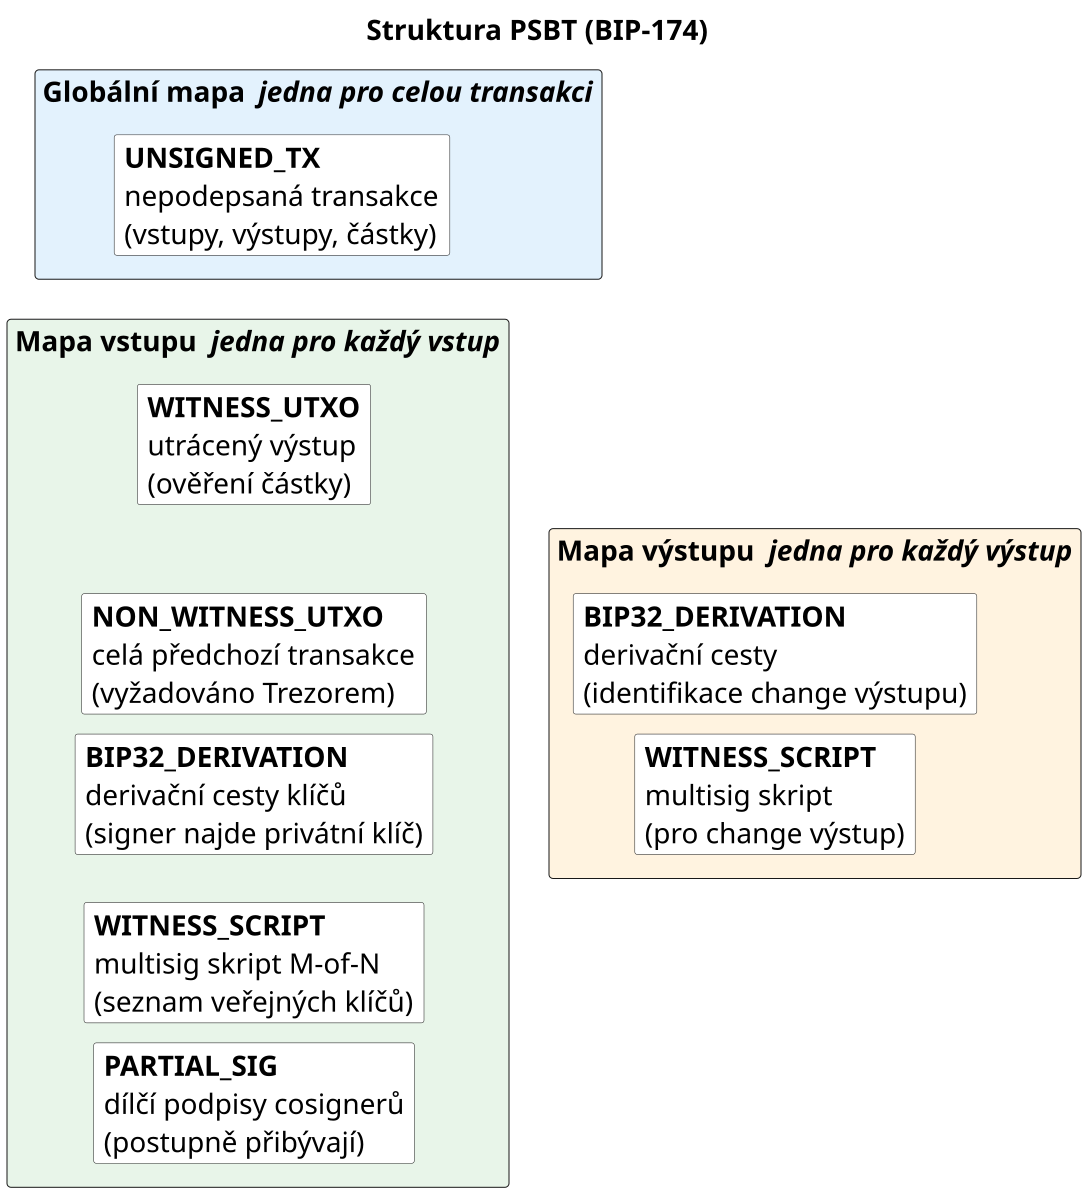
\includegraphics[width=\textwidth]{img/psbt-structure.pdf}
\caption{Struktura PSBT pro multisig transakci se dvěma vstupy a~dvěma výstupy.
Globální mapa obsahuje nepodepsanou transakci, mapy vstupů nesou data pro
podepisování a~mapa change výstupu obsahuje derivační cesty pro identifikaci
vlastního výstupu.}
\label{fig:psbt-structure}
\end{figure}

Standard rozlišuje šest rolí v~životním cyklu PSBT. Tyto role představují
logické kroky zpracování -- jedna entita může zastávat více rolí současně:
\begin{enumerate}
  \item \textbf{Creator} vytvoří PSBT s~globální transakcí (vstupy a~výstupy)
    a~prázdnými mapami vstupů a~výstupů.
  \item \textbf{Updater} doplní mapy o~metadata potřebná k~podpisu -- UTXO
    informace, derivační cesty, witness skripty. Po tomto kroku PSBT obsahuje
    vše, co signer potřebuje k~vytvoření podpisů.
  \item \textbf{Signer} na základě derivačních cest v~mapách vstupů najde
    příslušné privátní klíče a~přidá podpisy. V~rámci multisig schématu může
    PSBT projít postupně přes více signerů, z~nichž každý přidá svůj podpis.
  \item \textbf{Combiner} sloučí více částečně podepsaných PSBT (od různých
    signerů) do jednoho PSBT obsahujícího všechny podpisy.
  \item \textbf{Finalizer} zkontroluje, že všechny potřebné podpisy jsou
    přítomny, sestaví finální witness data a~odstraní pomocná metadata.
  \item \textbf{Extractor} extrahuje finální podepsanou transakci připravenou
    k~odeslání do sítě.
\end{enumerate}

Klíčovou vlastností PSBT je, že tyto role nemusí zastávat jedna entita --
naopak, celý smysl formátu spočívá v~rozdělení procesu podepisování mezi
více nezávislých systémů. Obrázek~\ref{fig:psbt-lifecycle} zachycuje
typický průběh zpracování PSBT pro multisig transakci.

\begin{figure}[htbp]
\centering
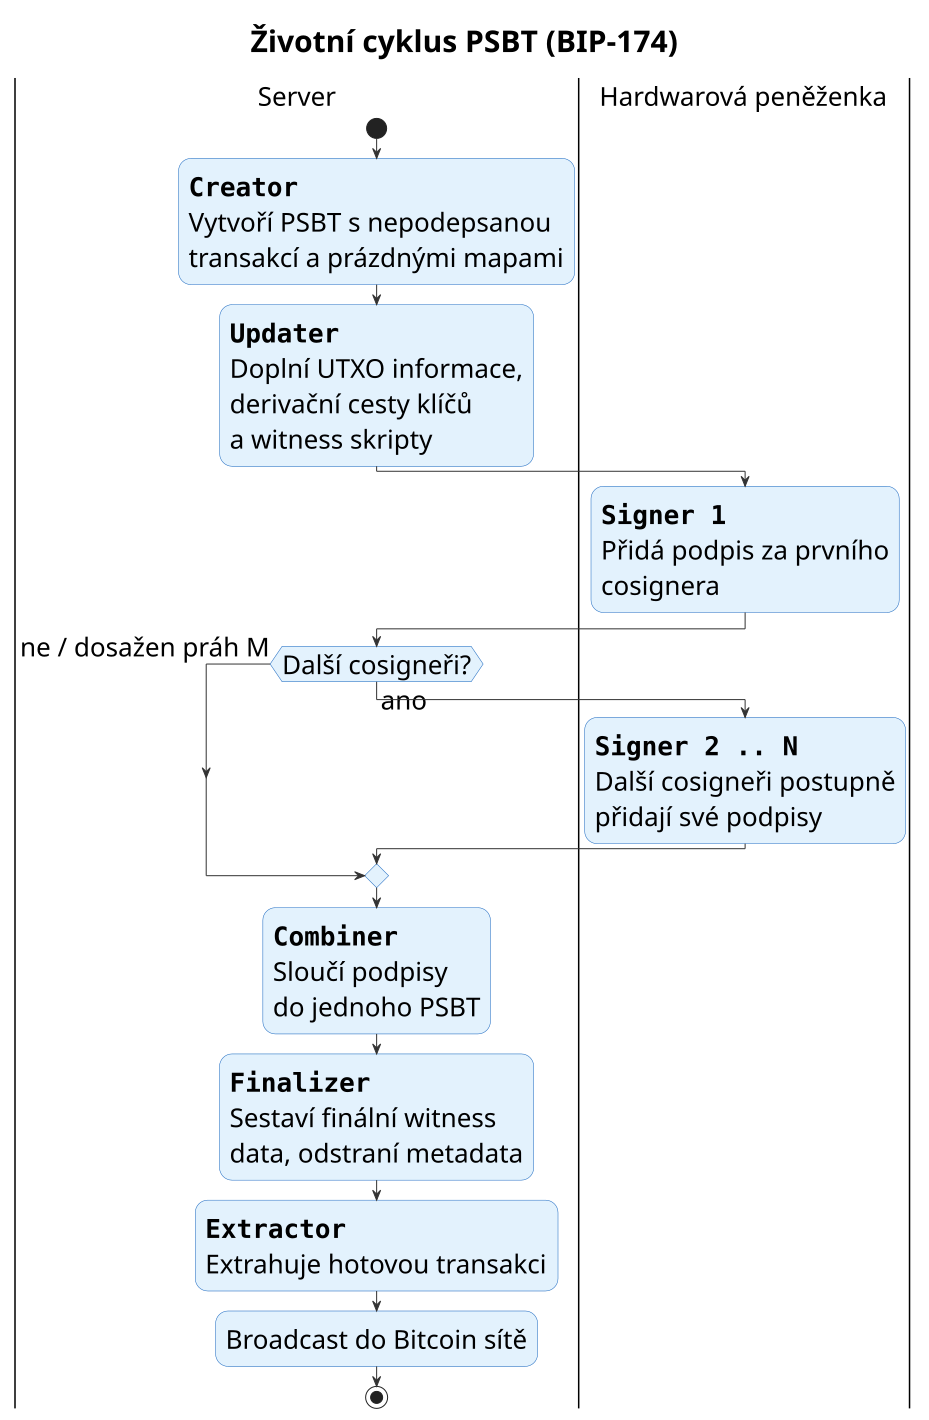
\includegraphics[width=0.85\textwidth]{img/psbt-lifecycle.pdf}
\caption{Životní cyklus PSBT pro multisig transakci. Serverová služba
zastává role Creator a~Updater, shromažďuje podpisy a~aktualizuje parametry
pro další cosignery. Trezor Connect interně provádí finalizaci (Combiner,
Finalizer) a~vrací kompletní serializovanou transakci (Extractor).
Hardwarové peněženky cosignerů vystupují jako Signeři.}
\label{fig:psbt-lifecycle}
\end{figure}

Celý proces probíhá následovně. Serverová služba nejprve vytvoří PSBT
s~nepodepsanou transakcí (\textbf{Creator}) -- na základě zvolených
UTXO vstupů, cílové adresy a~částky sestaví kostru transakce. Poté
do map vstupů doplní veškerá metadata potřebná k~podpisu
(\textbf{Updater}): referenční UTXO (aby signer mohl ověřit utrácené
částky), derivační cesty klíčů (aby hardwarová peněženka věděla, kterým
privátním klíčem podepsat), a~pro multisig vstupy i~kompletní witness
skript (aby signer znal seznam všech cosignerů a~požadovaný práh).
Do map výstupů přidá derivační cesty pro change výstup, aby peněženka
mohla ověřit, že vrácení změny směřuje zpět na vlastní adresu.

Takto připravené PSBT server odešle na mobilní aplikaci prvního
cosignera. Ta předá PSBT hardwarové peněžence (\textbf{Signer~1}),
která na svém displeji zobrazí detaily transakce -- cílovou adresu,
částku, poplatek. Po potvrzení uživatelem peněženka přidá svůj dílčí
podpis do polí \texttt{PARTIAL\_SIG} v~mapách vstupů. Částečně podepsané
PSBT se vrátí na server.

U~singlesig transakce je v~tomto okamžiku PSBT kompletní. U~multisig
transakce (např.\ 2-of-3) server čeká na podpis dalšího cosignera.
Druhý cosigner obdrží totéž PSBT (nyní již s~jedním podpisem), přidá
svůj podpis (\textbf{Signer~2}) a~PSBT se opět vrátí na server.

Jakmile server shromáždí požadovaný počet podpisů~$M$, předá je
poslednímu podepisujícímu Trezoru prostřednictvím Trezor Connect
parametrů. Trezor Connect interně provede sloučení podpisů
(\textbf{Combiner}), sestavení finální witness dat (\textbf{Finalizer})
a~extrakci kompletní podepsané transakce (\textbf{Extractor}),
kterou vrátí v~callback jako \texttt{serializedTx} připravenou
k~odeslání do Bitcoinové sítě.
Konkrétní mapování rolí na komponenty
systému popisujeme v~kapitole o~návrhu architektury.

\subsection{Výstupní deskriptory}
\label{sec:descriptors}

Výstupní deskriptory~\citep{BIP380} kompaktně popisují, jaké skripty
peněženka generuje. Pro multisig je podstatný formát z~BIP-383~\citep{BIP383}:

\begin{code}
wsh(sortedmulti(M,[fingerprint/path]xpub/0/*,...))
\end{code}

Tento deskriptor říká: \enquote{vytvořte P2WSH výstup obsahující M-of-N multisig
skript, kde jsou veřejné klíče seřazeny lexikograficky (dle BIP-67).} Každý
klíč je specifikován svým kořenovým otiskem (fingerprint), derivační cestou
a~rozšířeným veřejným klíčem (\texttt{xpub}). Suffix \texttt{/0/*} označuje
odvození přijímacích adres (resp.\ \texttt{/1/*} pro change adresy).

V~praxi to funguje tak, že uživatel vytvoří multisig peněženku
v~desktopové aplikaci (např.\ Sparrow Wallet~\citep{SparrowWallet}),
exportuje deskriptor a~vloží ho do mobilní peněženky. Z~deskriptoru
peněženka odvodí adresy, práh podpisů i~klíče cosignerů.


%%% -----------------------------------------------------------------
\section{Multisignature transakce}
\label{sec:multisig}

U~multisig transakcí je k~utracení prostředků potřeba M~podpisů z~N~klíčů
(schéma M-of-N). Oproti singlesig, kde zcizení jednoho klíče stačí ke ztrátě
prostředků, musí útočník u~multisig získat alespoň M~klíčů.

\subsection{Bezpečnostní výhody}
\label{sec:multisig-security}

Odpadá tak single point of failure. Praktické výhody:

\begin{itemize}
  \item \textbf{Ochrana proti krádeži}: Ani kompromitace jednoho klíče (např.\
    při zcizení hardwarové peněženky) neumožní útočníkovi provést transakci.
  \item \textbf{Odolnost proti ztrátě}: Ve schématu 2-of-3 může uživatel
    ztratit jeden klíč a~stále má dostatek klíčů k~obnovení přístupu
    k~prostředkům.
  \item \textbf{Geografická distribuce}: Jednotlivé klíče mohou být uloženy na
    různých místech, čímž se snižuje riziko současné ztráty.
\end{itemize}

\subsection{Případy užití}
\label{sec:multisig-usecases}

Multisig schémata nacházejí uplatnění v~různých scénářích:

\begin{itemize}
  \item \textbf{Sdílená správa} (shared custody): Schéma 2-of-3 umožňuje
    například rodinné správě prostředků, kde k~provedení transakce je potřeba
    souhlas alespoň dvou ze tří členů rodiny.
  \item \textbf{Dědění}: Pověřenec (právník, notář) drží jeden z~klíčů, který
    v~kombinaci s~klíčem dědice umožní přístup k~prostředkům po úmrtí majitele.
  \item \textbf{Firemní treasury}: Schéma 3-of-5 nebo vyšší zajišťuje, že
    firemní prostředky nemohou být odeslány bez souhlasu více odpovědných osob.
  \item \textbf{Osobní bezpečnost}: Jednotlivec uloží klíče 2-of-3 schématu do
    tří různých hardwarových peněženek na třech geograficky oddělených místech.
\end{itemize}

\subsection{Implementace pomocí P2WSH}
\label{sec:p2wsh-multisig}

V~současné implementaci Bitcoinu se nativní SegWit multisig transakce realizují
pomocí typu výstupu P2WSH~\citep{BIP141}. Výstupní skript obsahuje 32bajtový
SHA-256 hash tzv.\ witness skriptu, který definuje podmínky utrácení.

Pro M-of-N multisig má witness skript následující strukturu:
\begin{center}
\texttt{OP\_M <pubkey\_1> <pubkey\_2> ... <pubkey\_N> OP\_N OP\_CHECKMULTISIG}
\end{center}

Při utrácení takového výstupu musí witness data obsahovat M~validních podpisů
a~kompletní witness skript. Virtuální velikost vstupu multisig transakce je
výrazně větší než u~singlesig, což se projeví ve vyšších poplatcích.

Velikost vstupu ve virtuálních bajtech (vBytes) se dle
BIP-141~\citep{BIP141} vypočítá jako:
\[
  \text{vSize} = \text{base\_size} + \lceil \text{witness\_size} / 4 \rceil
\]
kde \emph{base\_size} je velikost newitness části vstupu (41~bajtů: outpoint
36~B, sequence 4~B a~délka skriptu 1~B) a~\emph{witness\_size} je velikost
witness dat. Pro M-of-N multisig vstup witness data obsahují: úvodní
\texttt{OP\_0} a~délky polí (přibližně 6~B), M~podpisů (každý maximálně
73~B: DER-kódovaný podpis 71--72~B plus push opcode) a~kompletní witness
skript s~N~veřejnými klíči (každý 34~B: 33~B komprimovaný klíč plus push
opcode). Celkově tedy:
\[
  \text{vSize}_{\text{input}} \approx 41 + \frac{6 + 73 \cdot M + 34 \cdot N}{4} \text{~vB}
\]
Například pro schéma 2-of-3 je odhadovaná velikost jednoho vstupu přibližně
$41 + (6 + 146 + 102)/4 \approx 105$~vB.


%%% -----------------------------------------------------------------
\section{Hardwarové peněženky}
\label{sec:hw-wallets}

Hardwarové peněženky uchovávají privátní klíče na izolovaném zařízení --
klíče ho nikdy neopouštějí. Na rozdíl od softwarových peněženek, kde jsou
klíče v~paměti počítače nebo telefonu a~hrozí jejich zcizení malwarem,
hardwarová peněženka podepisuje transakce ve vlastním prostředí. Uživatel
na displeji zařízení vidí adresu a~částku a~podepisování potvrdí fyzicky.

Na trhu existuje několik hardwarových peněženek s~podporou Bitcoinu.
Tyto peněženky se liší nejen hardwarem a~bezpečnostním modelem, ale
především \textbf{nemají jednotné rozhraní} pro komunikaci s~aplikacemi
třetích stran -- integrace s~každou peněženkou tak představuje
samostatnou implementační práci. Níže popisujeme nejrozšířenější
z~nich a~zdůvodňujeme volbu Trezoru.

\subsection{Trezor}
\label{sec:trezor}

Trezor, vyvinutý českou společností SatoshiLabs, patří mezi nejrozšířenější
hardwarové peněženky na trhu. Aktuální modelová řada zahrnuje několik zařízení
-- od Trezor Safe 3 přes Safe 5 s~barevným dotykovým displejem až po nejnovější
Safe 7, který jako první v~řadě podporuje bezdrátovou komunikaci
prostřednictvím Bluetooth a~NFC. Starší modely se připojují výhradně přes USB.
Všechna zařízení podporují protokol Bitcoin včetně SegWit a~multisig
transakcí.

Důležité je rozlišovat kompatibilitu s~mobilními zařízeními. Aplikace Trezor
Suite Mobile, která je nezbytná pro deeplink komunikaci, podporuje pouze novější
modely: Trezor Model~T, Safe~3, Safe~5 a~Safe~7. Starší model
\textbf{Trezor One} (první generace s~micro-USB konektorem) mobilní aplikaci
nepodporuje a~lze jej použít pouze s~desktopovou verzí Trezor Suite.
Pro testování a~provoz naší aplikace je tedy vyžadován minimálně Trezor Model~T.

Pro integraci s~aplikacemi třetích stran slouží rozhraní
\textbf{Trezor Connect}~\citep{TrezorConnect}. Toto API poskytuje
JavaScriptové rozhraní zprostředkovávající komunikaci mezi webovou nebo
mobilní aplikací a~hardwarovým zařízením. Na mobilních zařízeních Android
komunikace probíhá prostřednictvím \emph{deeplinků} -- speciálních URL,
které otevřou aplikaci Trezor Suite Mobile s~parametry transakce; po
potvrzení uživatelem na zařízení se podepsaná data vrátí zpět volající
aplikaci. Klíčové operace zahrnují \texttt{getPublicKey} (export
rozšířeného veřejného klíče pro danou derivační cestu) a~\texttt{signTransaction}
(podepsání transakce s~parametry specifickými pro daný typ výstupu).

\subsection{Ledger}
\label{sec:ledger}

Ledger je francouzský výrobce hardwarových peněženek s~modely Ledger Nano S
Plus, Nano X (s~Bluetooth) a~Ledger Stax. Zařízení používají proprietární
operační systém BOLOS běžící na bezpečnostním čipu (Secure Element).
Ledger podporuje Bitcoin včetně SegWit a~multisig.

Pro integraci s~aplikacemi třetích stran Ledger poskytuje Ledger Live SDK,
které však primárně cílí na webové a~desktopové aplikace. Na mobilních
zařízeních je komunikace možná přes Bluetooth (Nano X), avšak vyžaduje
implementaci vlastního transportního protokolu. Ledger neposkytuje
deeplink API srovnatelné s~Trezor Connect, což komplikuje integraci
z~mobilních aplikací třetích stran.

\subsection{Coldcard}
\label{sec:coldcard}

Coldcard od kanadské společnosti Coinkite je hardwarová peněženka zaměřená
výhradně na Bitcoin. Je navržena pro maximální bezpečnost -- podporuje
plně \emph{air-gapped} provoz, kdy zařízení nikdy nemusí být připojeno
k~počítači ani telefonu. Transakce se přenášejí prostřednictvím microSD
karty ve formátu PSBT.

Coldcard neposkytuje žádné API ani SDK pro přímou komunikaci z~mobilní
aplikace. Integrace je možná pouze přes manuální přenos PSBT souborů
(microSD nebo NFC u~novějších modelů), což je pro mobilní peněženku
s~automatizovaným workflow nevhodné.

\subsection{BitBox02}
\label{sec:bitbox02}

BitBox02 od švýcarské společnosti Shift Crypto je kompaktní hardwarová
peněženka s~dotykovými senzory pro potvrzování transakcí. Zařízení
komunikuje přes USB-C a~nabízí open-source firmware.

Pro integraci BitBox02 poskytuje vlastní SDK komunikující přes WebSocket
protokol a~USB HID. Mobilní SDK existuje, ale je primárně určeno pro
vlastní aplikaci BitBoxApp. Integrace z~aplikace třetí strany na Androidu
by vyžadovala implementaci USB HID komunikace a~proprietárního protokolu.

\subsection{Shrnutí a volba Trezoru}

Z~uvedených hardwarových peněženek Trezor jako jediný poskytuje deeplink
API umožňující mobilní aplikaci třetí strany iniciovat podepisování
bez implementace nízkoúrovňového komunikačního protokolu. Ledger vyžaduje
vlastní Bluetooth transport, Coldcard je navržen pro offline přenos
a~BitBox02 vyžaduje USB HID komunikaci. Trezor je navíc v~České republice
zdaleka nejrozšířenější hardwarovou peněženkou, což odpovídá cílovému
publiku této práce.


%%% -----------------------------------------------------------------
\section{Přehled existujících řešení}
\label{sec:existing-solutions}

Níže srovnáváme sedm existujících peněženek z~hlediska podpory multisig
transakcí, coin control a~integrace s~hardwarovými peněženkami.

\subsection{Trezor Suite}
\label{sec:trezor-suite}

Trezor Suite~\citep{TrezorSuite} je oficiální aplikace od společnosti
SatoshiLabs pro správu prostředků na zařízeních Trezor. Je dostupná jako
desktopová aplikace pro Windows, macOS a~Linux, jako webová aplikace
a~v~mobilní verzi Trezor Suite Mobile pro Android a~iOS.

Aplikace nabízí přehledné uživatelské rozhraní, správu více účtů, plnou
podporu coin control s~vizualizací UTXO a~integraci s~burzami pro nákup
a~prodej kryptoměn. Trezor Suite podporuje všechny typy SegWit adres včetně
P2WPKH a~Taproot.

\textbf{Omezení}: Trezor Suite neposkytuje nativní správu multisig peněženek.
Uživatel nemůže v~aplikaci vytvořit multisig konfiguraci, importovat
deskriptor ani koordinovat podepisování s~více cosignery. Pro multisig
transakce je nutné použít aplikaci třetí strany (např.\ Electrum nebo Sparrow),
která komunikuje se zařízením Trezor prostřednictvím Trezor Connect. Mobilní
verze Trezor Suite Lite navíc nabízí pouze omezenou podmnožinu funkcí
desktopové verze.

\subsection{Sparrow Wallet}
\label{sec:sparrow}

Sparrow Wallet~\citep{SparrowWallet} je desktopová Bitcoin peněženka zaměřená
na bezpečnost, transparentnost a~pokročilé funkce. Aplikace je dostupná pro
Windows, macOS a~Linux a~je vydávána pod open-source licencí Apache 2.0.

Sparrow nabízí pravděpodobně nejkomplexnější podporu multisig transakcí ze
všech analyzovaných řešení. Uživatel může přímo v~aplikaci vytvořit multisig
konfiguraci M-of-N s~libovolnou kombinací klíčů -- z~hardwarových peněženek
různých výrobců (Trezor, Ledger, Coldcard, aj.), ze softwarových klíčů nebo
z~importovaných \texttt{xpub} klíčů. Aplikace generuje výstupní deskriptor,
který lze exportovat pro použití v~jiných peněženkách.

Další silné stránky zahrnují detailní coin control s~možností manuálního
označování (labeling) UTXO, vizualizaci transakčního grafu, analýzu soukromí,
podporu PSBT a~možnost připojení k~vlastnímu Bitcoin uzlu nebo serveru Electrum.

\textbf{Omezení}: Sparrow Wallet je dostupný \emph{výhradně jako desktopová
aplikace}. Neexistuje mobilní verze pro Android ani iOS. Uživatel, který chce
spravovat svou multisig peněženku mimo dosah stolního počítače, nemá tuto
možnost.

\subsection{Liana}
\label{sec:liana}

Liana~\citep{LianaWallet} je peněženka vyvíjená společností Wizardsardine,
která využívá jazyk Miniscript pro definici pokročilých podmínek utrácení.
Hlavní inovací je podpora \emph{časově zamčené obnovy} (timelocked recovery) --
uživatel může definovat záložní klíč, který se aktivuje po uplynutí zadaného
časového intervalu, pokud primární klíč nebyl použit.

Tento přístup řeší problém dědění a~obnovy bez nutnosti důvěry třetí straně.
Liana podporuje integraci s~hardwarovými peněženkami Ledger a~některými dalšími
zařízeními.

\textbf{Omezení}: Liana je dostupná pouze jako desktopová aplikace. Mobilní
verze neexistuje. Podpora hardwarových peněženek nezahrnuje zařízení Trezor,
což ji činí nepoužitelnou pro uživatele, kteří svou infrastrukturu klíčů
postavili na zařízeních Trezor. Multisig v~tradičním smyslu (M-of-N) není
primárním zaměřením aplikace -- místo toho se Liana soustředí na Miniscript
politiky, které mohou být pro běžného uživatele obtížně srozumitelné.

\subsection{BlueWallet}
\label{sec:bluewallet}

BlueWallet~\citep{BlueWallet} je open-source mobilní peněženka dostupná pro
Android a~iOS. Nabízí přehledné uživatelské rozhraní a~širokou škálu funkcí
včetně podpory Lightning Network.

BlueWallet obsahuje funkci \emph{Multisig Vault}, která umožňuje vytvoření
multisig peněženky přímo v~mobilní aplikaci. Uživatel může definovat schéma
M-of-N a~přidat klíče ze seed frází nebo importovaných \texttt{xpub} klíčů.
Aplikace rovněž podporuje coin control s~možností zmrazení (freeze) jednotlivých
UTXO a~export/import PSBT.

\textbf{Omezení}: Integrace s~hardwarovými peněženkami je omezená na komunikaci
prostřednictvím QR kódů nebo sdílení souborů PSBT. BlueWallet nepodporuje
přímé propojení s~Trezorem přes USB nebo deeplink protokol. Proces podepisování
s~hardwarovou peněženkou je tak vícekrokový a~vyžaduje manuální přenos dat
mezi aplikacemi, což zhoršuje uživatelský komfort a~zvyšuje riziko chyb.

\subsection{Nunchuk}
\label{sec:nunchuk}

Nunchuk~\citep{Nunchuk} je peněženka navržená primárně pro multisig správu
Bitcoinu. Je dostupná jako mobilní aplikace pro Android a~iOS i~jako desktopová
aplikace. Nunchuk podporuje širokou škálu hardwarových peněženek včetně Trezor,
Ledger, Coldcard a~BitBox.

Aplikace nabízí intuitivní průvodce vytvořením multisig peněženky, správu
klíčů s~možností testování podpisů (health check), kolaborativní podepisování
přes cloud synchronizaci a~podporu coin control. Nunchuk rovněž implementuje
koncept \emph{inheritance planning} s~využitím časových zámků.

\textbf{Omezení}: Pokročilé funkce Nunchuku, včetně kolaborativního
podepisování, air-gapped klíčů a~inheritance planningu, jsou dostupné pouze
v~rámci placeného předplatného (Nunchuk Premium). Bezplatná verze omezuje počet
klíčů a~peněženek. Tento model předplatného může být překážkou pro uživatele,
kteří preferují plně otevřená řešení bez závislosti na službách třetí strany.
Navíc cloudová synchronizace, byť end-to-end šifrovaná, přidává závislost
na~externí infrastruktuře provozovatele.

\subsection{Electrum}
\label{sec:electrum}

Electrum~\citep{Electrum} je jedna z~nejstarších a~nejpoužívanějších
Bitcoinových peněženek, aktivně vyvíjená od roku 2011. Desktopová verze nabízí
kompletní sadu pokročilých funkcí: multisig peněženky s~libovolným schématem
M-of-N, detailní coin control, integraci s~hardwarovými peněženkami (Trezor,
Ledger, Coldcard), podporu PSBT, Lightning Network a~připojení k~vlastnímu
Electrum serveru.

\textbf{Omezení}: Electrum má sice verzi pro Android, ta však nabízí výrazně
omezenou funkčnost oproti desktopové verzi. Mobilní verze nepodporuje multisig
peněženky, integraci s~hardwarovými peněženkami ani coin control. Uživatel je
tak na mobilním zařízení omezen na základní singlesig operace, což výrazně
snižuje hodnotu mobilní verze pro naše cílové použití.

\subsection{Wasabi Wallet}
\label{sec:wasabi}

Wasabi Wallet~\citep{WasabiWallet} je desktopová Bitcoin peněženka zaměřená
především na ochranu soukromí uživatele. Její hlavní funkcí je implementace
protokolu CoinJoin (ve variantě WabiSabi), který umožňuje společné míchání
transakcí více uživatelů za účelem ztížení analýzy blockchainu.

Wasabi nabízí automatický výběr UTXO optimalizovaný pro soukromí, integraci
s~Tor sítí pro anonymní komunikaci a~přehledné označování prostředků podle
úrovně soukromí (red/yellow/green shielding).

\textbf{Omezení}: Wasabi Wallet je dostupná \emph{výhradně jako desktopová
aplikace} pro Windows, macOS a~Linux. Mobilní verze neexistuje. Aplikace rovněž
nepodporuje multisignature transakce -- zaměřuje se výhradně na singlesig
operace s~důrazem na soukromí. Pro uživatele hledající kombinaci multisig
a~mobilní platformy tak Wasabi nepředstavuje řešení.


%%% -----------------------------------------------------------------
\section{Srovnání a identifikace nedostatků}
\label{sec:comparison}

Tabulka~\ref{tab:wallet-comparison} shrnuje klíčové vlastnosti analyzovaných
peněženek.

\begin{table}[htbp]
\centering
\caption{Srovnání existujících Bitcoinových peněženek}
\label{tab:wallet-comparison}
\footnotesize
\begin{tabular}{|l|c|c|c|c|c|c|}
\hline
\textbf{Peněženka} & \textbf{Desk.} & \textbf{Mobil} & \textbf{Multisig} & \textbf{Coin ctrl} & \textbf{HW peněž.} & \textbf{Licence} \\
\hline
Trezor Suite   & Ano & Ano\textsuperscript{*} & Ne  & Ano & Trezor    & Propriet. \\
Sparrow        & Ano & Ne                      & Ano & Ano & Více      & Apache~2.0 \\
Liana          & Ano & Ne                      & Část.\textsuperscript{$\dagger$} & Ne  & Jiné & MIT \\
BlueWallet     & Ne  & Ano                     & Ano & Ano & QR/PSBT   & MIT \\
Nunchuk        & Ano & Ano                     & Ano & Ano & Více      & Propriet.\textsuperscript{$\ddagger$} \\
Electrum       & Ano & Ano\textsuperscript{*}  & Ano\textsuperscript{*} & Ano\textsuperscript{*} & Více & MIT \\
Wasabi         & Ano & Ne                      & Ne  & Ano & Ne        & MIT \\
\hline
\textbf{Naše řeš.} & Ne & \textbf{Ano} & \textbf{Ano} & \textbf{Ano} & \textbf{Trezor} & --- \\
\hline
\end{tabular}
\normalsize

\smallskip
\footnotesize
\textsuperscript{*}~Mobilní verze s~omezenou funkcionalitou. \\
\textsuperscript{$\dagger$}~Miniscript politiky namísto tradičního M-of-N multisig. \\
\textsuperscript{$\ddagger$}~Pokročilé funkce vyžadují placené předplatné. \\
\normalsize
\end{table}

Ze srovnání vyplývá:

\begin{enumerate}
  \item \textbf{Desktopová řešení dominují v~pokročilých funkcích}:
    Nejkomplexnější multisig podporu nabízejí Sparrow a~Electrum, obě primárně
    desktopové aplikace. Sparrow, který považujeme za referenční řešení
    z~hlediska UX multisig workflow, nemá vůbec mobilní verzi.

  \item \textbf{Mobilní řešení mají omezenou integraci s~HW peněženkami}:
    BlueWallet sice podporuje multisig na mobilu, ale komunikace s~hardwarovou
    peněženkou probíhá pouze přes QR kódy a~manuální sdílení PSBT souborů,
    bez přímé integrace přes deeplink nebo USB.

  \item \textbf{Nunchuk se nejvíce blíží cílové specifikaci}, avšak jeho
    obchodní model s~placeným předplatným pro pokročilé funkce a~závislost na
    cloudové synchronizaci představují omezení pro uživatele, kteří preferují
    plně otevřené a~nezávislé řešení.

  \item \textbf{Žádné existující řešení nekombinuje} na platformě Android
    nativní multisig správu, coin control a~přímou integraci s~hardwarovou
    peněženkou Trezor prostřednictvím Trezor Connect API.
\end{enumerate}

Tato mezera je hlavní motivací pro aplikaci navrhovanou v~této práci,
která nabídne:

\begin{itemize}
  \item Plnou podporu multisignature transakcí ve schématu M-of-N s~využitím
    standardu BIP-174~\cite{BIP174} (PSBT) pro koordinaci podepisování.
  \item Integraci s~hardwarovou peněženkou Trezor prostřednictvím Trezor
    Connect API a~deeplink protokolu, bez nutnosti manuálního přenosu dat.
  \item Funkci coin control umožňující uživateli ručně vybírat UTXO při tvorbě
    transakcí.
  \item Bezpečnostní model, ve kterém privátní klíče nikdy neopouštějí
    hardwarové zařízení a~serverová část systému pracuje výhradně
    s~veřejnými klíči.
\end{itemize}

%%% -----------------------------------------------------------------
\section{Analýza technických přístupů}
\label{sec:analyza-pristupu}

Předchozí sekce identifikovaly mezeru na trhu -- absenci mobilní Bitcoinové
peněženky, která by kombinovala multisig správu, coin control a~přímou
integraci s~hardwarovou peněženkou Trezor. Než přistoupíme ke specifikaci
požadavků, je nutné analyzovat technické přístupy ke klíčovým problémům,
které implementace takové aplikace přináší. Tato sekce rozebírá tři
hlavní rozhodnutí: jakým způsobem komunikovat s~hardwarovým zařízením,
jak řešit správu multisig peněženek a~jaký formát zvolit pro koordinaci
podepisování. U~každého rozhodnutí uvádíme zvažované alternativy, jejich
výhody a~nevýhody a~zdůvodňujeme zvolenou variantu.


\subsection{Komunikace s~hardwarovou peněženkou Trezor}
\label{sec:analyza-trezor}

Zásadní architektonickou otázkou je, jakým způsobem bude mobilní aplikace
na platformě Android komunikovat se zařízením Trezor za účelem podepisování
transakcí. Identifikovali jsme tři přístupy.

\subsubsection{Trezor Connect JavaScript SDK}

Oficiální integrační rozhraní Trezor Connect~\citep{TrezorConnect} je
distribuováno jako JavaScriptová knihovna (\texttt{@trezor/connect}), určená
pro prostředí webového prohlížeče a~Node.js. Knihovna abstrahuje veškerou
komunikaci se zařízením do jednoduchých volání -- vývojář zavolá funkci
\texttt{signTransaction} s~parametry transakce a~SDK se postará o~sestavení
USB zpráv, obsluhu stavového automatu i~zobrazení potvrzovacího dialogu.

Pro nativní platformu Android však oficiální SDK neexistuje. V~repozitáři
SatoshiLabs se nachází archivovaná Android knihovna, která ale neodpovídá
aktuálnímu firmware zařízení, nepokrývá novější typy transakcí (včetně
P2WSH multisig) a~není aktivně udržovaná. Tento přístup je proto pro
nativní Android aplikaci nepoužitelný.

\subsubsection{Přímá USB komunikace přes Android USB Host API}

Technicky je možné komunikovat se zařízením Trezor přímo prostřednictvím
Android USB Host API -- tedy stejným způsobem, jakým to interně dělá
aplikace Trezor Suite Mobile. Zařízení Trezor se na úrovni USB chová
jako HID zařízení a~komunikuje pomocí zpráv ve formátu Protocol Buffers.

Podepisování Bitcoinové transakce na Trezoru však není jednorázová
operace. Zařízení má omezenou paměť (řádově jednotky kilobajtů pro
pracovní data), a~proto nemůže přijmout celou transakci najednou.
Místo toho probíhá vícekrokový dialog mezi aplikací a~zařízením:

\begin{enumerate}
  \item Aplikace odešle zprávu \texttt{SignTx} s~počtem vstupů a~výstupů.
  \item Zařízení odpoví zprávou \texttt{TxRequest}, ve které si vyžádá
    konkrétní data -- například vstup č.~2 nebo kompletní předchozí transakci
    odkazovanou vstupem č.~0.
  \item Aplikace odpovídá zprávou \texttt{TxAck} s~požadovanými daty.
  \item Kroky 2--3 se opakují v~desítkách iterací, dokud zařízení nezíská
    všechna potřebná data a~nevygeneruje podpisy.
\end{enumerate}

\noindent
Implementace tohoto přístupu by vyžadovala:

\begin{itemize}
  \item \textbf{USB transportní vrstvu} -- protokol pracuje s~64bajtovými
    pakety, zprávy je nutné fragmentovat a~sestavovat.
  \item \textbf{Protocol Buffers definice} -- kompletní sada zpráv
    odpovídající aktuálnímu firmware (desítky typů zpráv).
  \item \textbf{Stavový automat podepisování} -- implementaci výše
    popsaného cyklu \texttt{SignTx}~$\to$~\texttt{TxRequest}~$\to$~\texttt{TxAck}
    včetně zpracování všech typů požadavků (vstupy, výstupy, předchozí
    transakce, metadata).
  \item \textbf{Multisig rozšíření} -- pro multisig transakce je navíc
    nutné předávat witness skripty a~derivační cesty všech cosignerů
    s~korektním řazením klíčů dle BIP-67~\citep{BIP67}.
\end{itemize}

\noindent
Hrubý odhad pracnosti je přibližně 20 pracovních dní. Zdrojový kód
aplikace Trezor Suite je sice veřejně dostupný, ale je publikován pod
licencí T-RSL (Trezor Restricted Source License)~\citep{TRSL}, která
explicitně zakazuje kopírování kódu do jiných projektů -- umožňuje
pouze čtení za účelem studia. Implementace by proto musela vzniknout
zcela od základu na základě veřejné dokumentace
protokolu~\citep{TrezorFirmwareDocs}.

\subsubsection{Deeplink protokol přes Trezor Suite Mobile}

Třetí možností je delegovat komunikaci se zařízením na aplikaci Trezor
Suite Mobile, která je na cílovém Android zařízení nainstalována. Mobilní
aplikace otevře Trezor Suite Mobile prostřednictvím deeplinku (speciální
URL schéma), předá parametry transakce (vstupy, výstupy, referenční
transakce) a~registruje adresu pro zpětné volání. Po potvrzení uživatelem
na displeji hardwarové peněženky Trezor Suite Mobile vrátí podepsaná data
zpět volající aplikaci prostřednictvím callback URL.

Výhodou tohoto přístupu je využití produkčně otestovaného a~průběžně
udržovaného kódu od SatoshiLabs, který pokrývá veškerou složitost USB
protokolu, stavového automatu i~podporu všech typů transakcí. Nevýhodou
je závislost na instalaci externí aplikace a~krátké přesměrování
uživatele mimo peněženku.

\subsubsection{Zhodnocení a volba}

Přímá USB komunikace by přinesla lepší uživatelský zážitek -- celý
proces podepisování by probíhal uvnitř jedné aplikace bez přepínání
kontextu. Představuje však přibližně 20~dní dodatečného vývoje
a~nutnost implementace složitého protokolu zcela od základu (kvůli
licenčním omezením). JavaScript SDK je pro Android nepoužitelné.
V~kontextu rozsahu bakalářské práce je delegování na Trezor Suite
Mobile prostřednictvím deeplinků pragmatickou volbou.

Architektura aplikace je navržena s~čistým interním rozhraním pro
podepisování (\emph{signing interface}), za kterým se v~aktuální verzi
skrývá deeplink komunikace s~Trezor Suite Mobile. Toto rozhraní
umožňuje v~budoucnu přidat přímou USB komunikaci jako alternativní
implementaci bez nutnosti změn ve zbytku systému.


\subsection{Správa multisig peněženek}
\label{sec:analyza-multisig}

Druhým klíčovým rozhodnutím je, jakým způsobem bude multisig peněženka
vytvořena a~nakonfigurována. Vytvoření multisig peněženky je netriviální
koordinační úloha -- je nutné:

\begin{enumerate}
  \item Shromáždit rozšířené veřejné klíče (\texttt{xpub}) od všech
    N~cosignerů, přičemž každý cosigner musí klíč exportovat ze svého
    vlastního hardwarového zařízení.
  \item Dohodnout se na parametrech peněženky: práhu M~(kolik podpisů
    je potřeba k~utracení), derivačních cestách dle BIP-48~\citep{BIP48}
    a~typu skriptu (P2WSH).
  \item Z~těchto parametrů vygenerovat výstupní deskriptor a~ověřit,
    že všichni cosigneři pracují se shodnou konfigurací.
  \item Odvodit sadu multisig adres a~ověřit je na blockchainu.
\end{enumerate}

Na desktopové platformě tento proces pokrývá Sparrow
Wallet~\citep{SparrowWallet} -- nabízí průvodce vytvořením multisig
peněženky, umožňuje přidávat klíče z~hardwarových peněženek různých
výrobců (Trezor, Ledger, Coldcard), generuje a~validuje deskriptory
a~exportuje je pro použití v~jiných peněženkách.

Implementace celého konfiguračního procesu přímo v~mobilní aplikaci
by vyžadovala: bezpečný protokol pro výměnu \texttt{xpub} klíčů mezi
cosignery (potenciálně přes QR kódy, NFC nebo síťovou komunikaci),
uživatelské rozhraní pro přidávání, odebírání a~verifikaci cosignerů,
a~generování deskriptorů s~validací dle BIP-380~\citep{BIP380}
a~BIP-383~\citep{BIP383}. Jedná se o~funkcionalitu, která by svým
rozsahem odpovídala samostatnému projektu.

Zvolený přístup proto odděluje \emph{konfiguraci} peněženky od
jejího \emph{provozu}. Uživatel vytvoří multisig peněženku
v~desktopové aplikaci (typicky Sparrow Wallet, který je open-source
pod licencí Apache~2.0), exportuje výstupní deskriptor ve
standardizovaném formátu \texttt{wsh(sortedmulti(...))} a~vloží
ho do mobilní aplikace. Z~deskriptoru aplikace odvodí všechny
potřebné parametry -- práh, klíče cosignerů, derivační cesty --
a~může začít s~provozem: zobrazováním zůstatků, vytvářením
transakcí, koordinací podepisování a~broadcastem.

Tento kompromis je záměrný. Konfigurace multisig peněženky se
provádí typicky jednou a~vyžaduje přístup ke všem cosignerům
současně. Provozní operace (odesílání, podepisování, sledování
stavu) se provádějí opakovaně a~právě pro ně je mobilní aplikace
nejpřínosnější.


\subsection{Koordinace podepisování pomocí PSBT}
\label{sec:analyza-psbt}

V~multisig schématu musí tutéž transakci postupně podepsat více cosignerů,
potenciálně na různých zařízeních a~v~různém čase. Klíčovou otázkou je,
v~jakém formátu transakci mezi cosignery distribuovat a~jak sbírat
dílčí podpisy.

\subsubsection{Vlastní formát}

Jednou z~možností je definovat vlastní datový formát (například JSON),
který by obsahoval parametry transakce a~pole pro podpisy. Tento přístup
by umožnil maximální flexibilitu, ale přinesl by zásadní nevýhodu:
ztrátu interoperability. Žádná jiná peněženka by nedokázala takový formát
zpracovat, a~uživatel by byl zcela závislý na jedné aplikaci pro celý
životní cyklus transakce.

\subsubsection{Standard PSBT (BIP-174)}

Standard PSBT (Partially Signed Bitcoin Transaction,
BIP-174~\citep{BIP174}), jehož strukturu jsme popsali
v~sekci~\ref{sec:psbt}, je navržen přesně pro tento účel. PSBT
je podporován hardwarovými peněženkami Trezor (prostřednictvím Trezor
Connect~\citep{TrezorConnect}), desktopovými peněženkami
Sparrow~\citep{SparrowWallet} a~Electrum~\citep{Electrum} i~dalšími
nástroji Bitcoinového ekosystému.

Volba PSBT zajišťuje, že aplikace zapadá do existujícího ekosystému.
Uživatel může například zahájit transakci v~mobilní aplikaci, exportovat
částečně podepsanou PSBT a~dokončit podepisování ve Sparrow na desktopu
-- nebo naopak. Tato interoperabilita je pro multisig workflow obzvláště
důležitá, neboť jednotliví cosigneři mohou používat různé peněženky.

Z~těchto důvodů volíme PSBT jako formát pro koordinaci podepisování.
Backendová služba vystupuje jako koordinátor: vytvoří PSBT s~kompletními
metadaty (role Creator a~Updater), distribuuje ji cosignerům k~podpisu,
sbírá dílčí podpisy a~po dosažení prahu~M provede finalizaci
a~broadcast do sítě.


\subsection{Shrnutí: rozsah vlastní implementace}
\label{sec:analyza-rozsah}

Na základě předchozí analýzy lze shrnout rozdělení odpovědností.
Aplikace \emph{sama implementuje}: konstrukci a~finalizaci PSBT
(BIP-174), derivaci adres z~veřejných klíčů (BIP-32), správu UTXO
a~coin control, odhad transakčních poplatků, koordinaci multisig
podepisování a~celé uživatelské rozhraní pro Android.
Aplikace \emph{deleguje}: vytváření multisig peněženek na desktopovou
aplikaci (Sparrow Wallet), podepisování transakcí na hardwarovou
peněženku Trezor prostřednictvím Trezor Suite Mobile a~přístup
k~blockchainovým datům na veřejná API (Blockstream Esplora
pro mainnet, Mempool.space pro testnet4).

Toto rozdělení odráží rozsah realizovatelný v~rámci bakalářské práce
a~přitom poskytuje kompletní a~použitelnou aplikaci pokrývající celý
operační cyklus -- od příjmu prostředků přes tvorbu a~koordinaci
transakcí až po broadcast do Bitcoinové sítě. Architektura je navržena
tak, aby delegované části (zejména podepisování) mohly být v~budoucnu
nahrazeny vlastní implementací bez zásahu do zbytku systému.

Na základě provedené analýzy nyní v~následující kapitole specifikujeme
požadavky na systém.

%%% Kapitola 2: Specifikace požadavků

\chapter{Specifikace požadavků}
\label{chap:specifikace}

Tato kapitola definuje požadavky na systém -- uživatelskou roli, uživatelské
příběhy (user stories), případy užití (use cases) a~z~nich odvozené funkční
a~nefunkční požadavky.

%%% -----------------------------------------------------------------------
\section{Uživatelské role}
\label{sec:role}

Systém definujeme pro jedinou uživatelskou roli -- \textbf{uživatele Bitcoinové
peněženky}. Tento uživatel vlastní hardwarovou peněženku Trezor a~chce prostřednictvím
mobilní aplikace na platformě Android spravovat své Bitcoinové prostředky. Uživatel
požaduje pokročilé funkce, které mu běžné mobilní peněženky neposkytují:

\begin{itemize}
  \item \textbf{Multisignature transakce} -- možnost vytvářet a~podepisovat transakce
        vyžadující souhlas více klíčů (schéma M-of-N).
  \item \textbf{Coin control} -- manuální výběr konkrétních nepoužitých výstupů
        (UTXO) při tvorbě transakcí.
  \item \textbf{Integrace s~hardwarovou peněženkou} -- veškeré podepisování transakcí
        probíhá výhradně na zařízení Trezor; server nikdy nedisponuje privátními klíči.
\end{itemize}

Předpokládáme, že uživatel má základní znalost fungování Bitcoinu a~je obeznámen
s~konceptem hardwarových peněženek. Systém nepočítá s~rolí administrátora ani
s~víceuživatelským režimem -- každá instance backendu obsluhuje jednoho uživatele
s~jeho účty.

%%% -----------------------------------------------------------------------
\section{Uživatelské příběhy}
\label{sec:user-stories}

Požadavky formulujeme jako uživatelské příběhy ve formátu
\emph{,,Jako uživatel chci \ldots, abych \ldots``}.

\begin{enumerate}
  \item \textbf{US1 -- Připojení Trezoru:}
        Jako uživatel chci připojit svou hardwarovou peněženku Trezor k~aplikaci,
        abych se mohl přihlásit a~aplikace automaticky nalezla mé aktivní účty.

  \item \textbf{US2 -- Zobrazení zůstatku:}
        Jako uživatel chci vidět aktuální zůstatek svých Bitcoinových účtů v~BTC
        i~ve fiat měně, abych měl přehled o~stavu svých prostředků.

  \item \textbf{US3 -- Odeslání prostředků:}
        Jako uživatel chci odeslat Bitcoin na zadanou adresu s~volitelným nastavením
        poplatku, abych mohl provádět platby.

  \item \textbf{US4 -- Příjem prostředků:}
        Jako uživatel chci zobrazit svou přijímací adresu a~QR kód, abych mohl
        jednoduše přijímat platby.

  \item \textbf{US5 -- Manuální výběr UTXO:}
        Jako uživatel chci při tvorbě transakce ručně vybrat konkrétní UTXO
        (coin control), abych měl plnou kontrolu nad tím, které prostředky budou
        použity, a~mohl tak lépe chránit své soukromí.

  \item \textbf{US6 -- Import multisig deskriptoru:}
        Jako uživatel chci importovat deskriptor multisignature peněženky ve formátu
        \texttt{wsh(sortedmulti(\ldots))}, abych mohl v~aplikaci spravovat sdílenou
        peněženku vyžadující více podpisů.

  \item \textbf{US7 -- Vytvoření a~podepsání multisig transakce:}
        Jako uživatel chci vytvořit PSBT pro multisig peněženku a~podepsat jej svým
        Trezorem, abych mohl iniciovat transakci vyžadující souhlas více cosignerů.

  \item \textbf{US8 -- Zobrazení stavu PSBT:}
        Jako uživatel chci vidět stav rozpracovaných PSBT (počet shromážděných
        podpisů, chybějící podpisy), abych věděl, zda je transakce připravena
        k~odeslání.

  \item \textbf{US9 -- Doplnění podpisu k~existujícímu PSBT:}
        Jako uživatel chci přepnout účet a~doplnit svůj podpis k~rozpracovanému PSBT,
        abych jako další cosigner přispěl k~dosažení požadovaného prahu podpisů.

  \item \textbf{US10 -- Přepínání účtů:}
        Jako uživatel chci přepínat mezi svými singlesig a~multisig účty, abych mohl
        spravovat prostředky na různých peněženkách z~jedné aplikace.

  \item \textbf{US11 -- Historie transakcí:}
        Jako uživatel chci zobrazit historii odeslaných a~přijatých transakcí včetně
        jejich detailů, abych měl přehled o~pohybech na svém účtu.

  \item \textbf{US12 -- Odhad poplatků:}
        Jako uživatel chci vidět odhadovaný poplatek za transakci před jejím
        odesláním, abych se mohl rozhodnout, zda je poplatek přijatelný.
\end{enumerate}

%%% -----------------------------------------------------------------------
\section{Případy užití}
\label{sec:use-cases}

Z~user stories a~analýzy technických možností provedené
v~sekci~\ref{sec:analyza-pristupu} vycházejí následující případy užití.
Každý popisujeme strukturovaně: aktér, vstupní podmínky, hlavní scénář,
výstupní podmínky a~alternativní scénáře.

% ---- UC1 ----
\subsection{UC1: Připojení Trezoru a přihlášení}
\label{uc:login}

\begin{description}
  \item[Aktér:] Uživatel s~hardwarovou peněženkou Trezor.
  \item[Vstupní podmínky:] \hfill
    \begin{itemize}
      \item Na mobilním zařízení je nainstalována aplikace Trezor Suite Mobile.
      \item Backend systém je spuštěn a~dostupný po síti.
      \item Trezor je inicializován a~obsahuje seed.
    \end{itemize}
  \item[Hlavní scénář:] \hfill
    \begin{enumerate}
      \item Uživatel spustí aplikaci a~zvolí přihlášení.
      \item Aplikace zahájí export rozšířených veřejných klíčů (xpub)
            z~Trezoru přes Trezor Suite Mobile.
      \item Uživatel je přesměrován do aplikace Trezor Suite Mobile a~na
            Trezoru potvrdí export.
      \item Trezor Suite Mobile vrátí sadu xpub zpět do aplikace.
      \item Aplikace odešle xpub na backend, který provede account discovery
            (ověří, které účty mají transakční historii).
      \item Backend vytvoří peněženky pro účty s~nalezenou aktivitou, vydá
            přihlašovací token a~vrátí seznam nalezených účtů.
      \item Uživatel vybere účet ze seznamu a~aplikace zobrazí dashboard.
    \end{enumerate}
  \item[Výstupní podmínky:] Uživatel je přihlášen, aplikace zobrazuje jeho účty
    a~zůstatky.
  \needspace{5\baselineskip}
  \item[Alternativní scénáře:] \hfill
    \begin{itemize}
      \item \emph{Trezor Suite Mobile není nainstalována:} Aplikace zobrazí chybovou
            hlášku s~instrukcí k~instalaci.
      \item \emph{Žádný účet nemá aktivitu:} Backend nevytvoří žádnou peněženku;
            aplikace informuje uživatele, že nebyly nalezeny účty s~historií.
      \item \emph{Backend není dostupný:} Aplikace zobrazí chybovou hlášku o~nedostupnosti
            serveru.
    \end{itemize}
\end{description}

% ---- UC2 ----
\subsection{UC2: Odeslání singlesig transakce}
\label{uc:send-singlesig}

\begin{description}
  \item[Aktér:] Přihlášený uživatel s~kladným zůstatkem na singlesig účtu.
  \item[Vstupní podmínky:] \hfill
    \begin{itemize}
      \item Uživatel je přihlášen a~má vybraný singlesig účet.
      \item Na účtu je dostatečný zůstatek pro pokrytí částky i~poplatku.
    \end{itemize}
  \item[Hlavní scénář:] \hfill
    \begin{enumerate}
      \item Uživatel přejde na obrazovku odeslání a~zadá cílovou adresu (ručně nebo
            naskenováním QR kódu).
      \item Uživatel zadá částku v~BTC nebo ve zvolené fiat měně
            (CZK, USD nebo EUR; konkrétní měna se volí v~nastavení).
      \item Aplikace zobrazí odhadovaný poplatek na základě aktuálního stavu mempoolu.
      \item Uživatel volitelně aktivuje coin control a~vybere konkrétní UTXO
            (viz UC5, sekce~\ref{uc:coin-control}).
      \item Uživatel potvrdí odeslání.
      \item Backend sestaví transakci ve formátu P2WPKH~\cite{BIP84} a~připraví
            parametry pro Trezor Connect.
      \item Aplikace přesměruje uživatele do Trezor Suite Mobile k~podepsání
            transakce.
      \item Uživatel potvrdí transakci na Trezoru.
      \item Podepsaná transakce je vrácena do aplikace a~odeslána na backend.
      \item Backend provede broadcast transakce do Bitcoin sítě.
      \item Aplikace zobrazí potvrzení o~úspěšném odeslání.
    \end{enumerate}
  \item[Výstupní podmínky:] Transakce je odeslána do sítě, zůstatek na účtu je
    aktualizován.
  \item[Alternativní scénáře:] \hfill
    \begin{itemize}
      \item \emph{Nedostatečný zůstatek:} Aplikace zobrazí chybovou hlášku.
      \item \emph{Neplatná cílová adresa:} Aplikace upozorní uživatele na neplatný
            formát adresy.
      \item \emph{Uživatel odmítne podpis na Trezoru:} Transakce je zrušena.
    \end{itemize}
\end{description}

% ---- UC3 ----
\subsection{UC3: Import multisig peněženky}
\label{uc:import-multisig}

\begin{description}
  \item[Aktér:] Přihlášený uživatel, který má k~dispozici deskriptor multisig
    peněženky.
  \item[Vstupní podmínky:] \hfill
    \begin{itemize}
      \item Uživatel je přihlášen.
      \item Uživatel má k~dispozici platný deskriptor
            multisig peněženky vytvořený například v~programu
            Sparrow Wallet \cite{SparrowWallet}.
    \end{itemize}
  \item[Hlavní scénář:] \hfill
    \begin{enumerate}
      \item Uživatel otevře seznam multisig peněženek a~zvolí import nové peněženky.
      \item Uživatel vloží deskriptor (textovým vložením ze schránky nebo
            naskenováním QR kódu).
      \item Backend parsuje deskriptor dle BIP-380~\cite{BIP380} a~BIP-383~\cite{BIP383},
            extrahuje práh M, veřejné klíče cosignerů a~jejich derivační cesty
            dle BIP-48~\cite{BIP48}.
      \item Backend odvodí adresy P2WSH~\cite{BIP141} pro multisig peněženku
            a~provede discovery (prohledání adres dle gap limitu).
      \item Backend uloží konfiguraci peněženky a~vrátí informace o~peněžence
            (práh, počet cosignerů, derivované adresy).
      \item Aplikace zobrazí nově importovanou multisig peněženku v~seznamu účtů.
    \end{enumerate}
  \item[Výstupní podmínky:] Multisig peněženka je importována a~zobrazena v~seznamu
    účtů s~aktuálním zůstatkem.
  \item[Alternativní scénáře:] \hfill
    \begin{itemize}
      \item \emph{Neplatný deskriptor:} Backend vrátí chybu s~popisem problému;
            aplikace zobrazí hlášku s~detailem.
      \item \emph{Deskriptor neobsahuje xpub aktuálního účtu uživatele:}
            Backend import odmítne s~hláškou, že daný účet není cosignerem
            této multisig peněženky; aplikace chybu zobrazí.
    \end{itemize}
\end{description}

% ---- UC4 ----
\subsection{UC4: Vytvoření a podepsání multisig transakce}
\label{uc:multisig-sign}

\begin{description}
  \item[Aktér:] Přihlášený uživatel s~importovanou multisig peněženkou (práh 2-of-3).
  \item[Vstupní podmínky:] \hfill
    \begin{itemize}
      \item Uživatel je přihlášen a~má vybranou multisig peněženku.
      \item Na peněžence je dostatečný zůstatek.
      \item Uživatel je jedním z~cosignerů dané peněženky.
    \end{itemize}
  \item[Hlavní scénář:] \hfill
    \begin{enumerate}
      \item Uživatel přejde na obrazovku odeslání a~zadá cílovou adresu a~částku.
      \item Backend sestaví PSBT~\cite{BIP174} pro multisig transakci (typ P2WSH).
      \item Aplikace zobrazí detail PSBT s~informacemi o~transakci.
      \item Uživatel zvolí podepsání transakce (\emph{Sign with Trezor}).
      \item Aplikace přesměruje uživatele do Trezor Suite Mobile s~parametry pro
            podepisování multisig transakce (včetně derivační cesty dle
            BIP-48~\cite{BIP48}).
      \item Uživatel potvrdí podpis na Trezoru.
      \item Částečně podepsané PSBT je uloženo na backendu.
      \item Aplikace zobrazí stav PSBT -- 1~z~2 podpisů shromážděn.
      \item Druhý cosigner otevře rozpracované PSBT a~doplní svůj podpis
            (viz UC6, sekce~\ref{uc:psbt-status}).
      \item Po dosažení prahu (2~ze~3) je PSBT připraveno k~odeslání;
            uživatel zvolí broadcast a~backend transakci finalizuje
            a~odešle do Bitcoin sítě.
    \end{enumerate}
  \item[Výstupní podmínky:] Plně podepsaná transakce je odeslána do Bitcoin sítě.
  \item[Alternativní scénáře:] \hfill
    \begin{itemize}
      \item \emph{Práh podpisů není dosažen:} PSBT zůstává ve stavu ,,rozpracováno``;
            další cosigner může podpis doplnit později.
      \item \emph{Broadcast selže:} Aplikace zobrazí chybovou hlášku; PSBT zůstává
            uloženo pro opakovaný pokus.
    \end{itemize}
\end{description}

% ---- UC5 ----
\subsection{UC5: Manuální výběr UTXO (coin control)}
\label{uc:coin-control}

\begin{description}
  \item[Aktér:] Přihlášený uživatel s~více než jedním UTXO na účtu.
  \item[Vstupní podmínky:] \hfill
    \begin{itemize}
      \item Uživatel je přihlášen a~má na účtu alespoň dvě UTXO.
      \item Uživatel se nachází na obrazovce odeslání transakce.
    \end{itemize}
  \item[Hlavní scénář:] \hfill
    \begin{enumerate}
      \item Uživatel na obrazovce odeslání přepne výběr UTXO z~automatického
            na ruční (přepínač \emph{Automatic} / \emph{Manual}) a~zvolí úpravu
            výběru.
      \item Aplikace zobrazí seznam dostupných UTXO s~informacemi: částka,
            adresa, stav (potvrzeno, nepotvrzeno, rezervováno jiným
            rozpracovaným PSBT) a~datum bloku.
      \item Uživatel zaškrtnutím vybere jedno nebo více UTXO, která chce
            použít jako vstupy transakce.
      \item Uživatel výběr potvrdí a~vrátí se na obrazovku odeslání.
      \item Pokračuje v~sestavení a~odeslání transakce standardním postupem
            (viz UC2 nebo UC4); poplatek je přepočten při sestavení PSBT
            podle počtu vybraných vstupů.
    \end{enumerate}
  \item[Výstupní podmínky:] Transakce je sestavena výhradně z~uživatelem vybraných
    UTXO.
  \item[Alternativní scénáře:] \hfill
    \begin{itemize}
      \item \emph{Vybraná UTXO nepokrývají požadovanou částku:} Aplikace upozorní
            uživatele na nedostatečný součet vybraných UTXO.
      \item \emph{Uživatel zruší výběr:} Systém se vrátí k~automatickému výběru UTXO.
    \end{itemize}
\end{description}

% ---- UC6 ----
\subsection{UC6: Zobrazení stavu PSBT a doplnění podpisu}
\label{uc:psbt-status}

\begin{description}
  \item[Aktér:] Přihlášený uživatel, cosigner multisig peněženky.
  \item[Vstupní podmínky:] \hfill
    \begin{itemize}
      \item Na backendu existuje rozpracované PSBT s~alespoň jedním podpisem.
      \item Uživatel je jedním z~cosignerů, který dosud nepodepsal.
    \end{itemize}
  \item[Hlavní scénář:] \hfill
    \begin{enumerate}
      \item Uživatel přepne účet v~nastavení na odpovídajícího cosignera.
      \item Uživatel přejde na seznam rozpracovaných PSBT.
      \item Aplikace zobrazí detail PSBT: částka, poplatek, počet shromážděných
            podpisů a~seznam cosignerů s~vyznačením, kdo již podepsal.
      \item Uživatel zvolí doplnění podpisu.
      \item Aplikace přesměruje uživatele do Trezor Suite Mobile s~derivační cestou
            aktuálního cosignera.
      \item Uživatel potvrdí podpis na Trezoru.
      \item Backend aktualizuje PSBT o~nový podpis.
      \item Pokud je dosažen práh podpisů, PSBT je připraveno k~odeslání;
            uživatel zvolí broadcast a~backend transakci finalizuje a~odešle
            do sítě. V~opačném případě PSBT zůstává rozpracované pro dalšího
            cosignera.
    \end{enumerate}
  \item[Výstupní podmínky:] PSBT je aktualizováno o~nový podpis. Pokud byl dosažen
    práh a~uživatel zvolil broadcast, transakce je odeslána do sítě.
  \item[Alternativní scénáře:] \hfill
    \begin{itemize}
      \item \emph{Práh stále není dosažen:} PSBT zůstává ve stavu ,,rozpracováno``
            pro další cosignery.
    \end{itemize}
\end{description}

Přehled všech případů užití a~jejich vzájemných vazeb zachycuje diagram na
obrázku~\ref{fig:use-case}.

\begin{figure}[htbp]
\centering
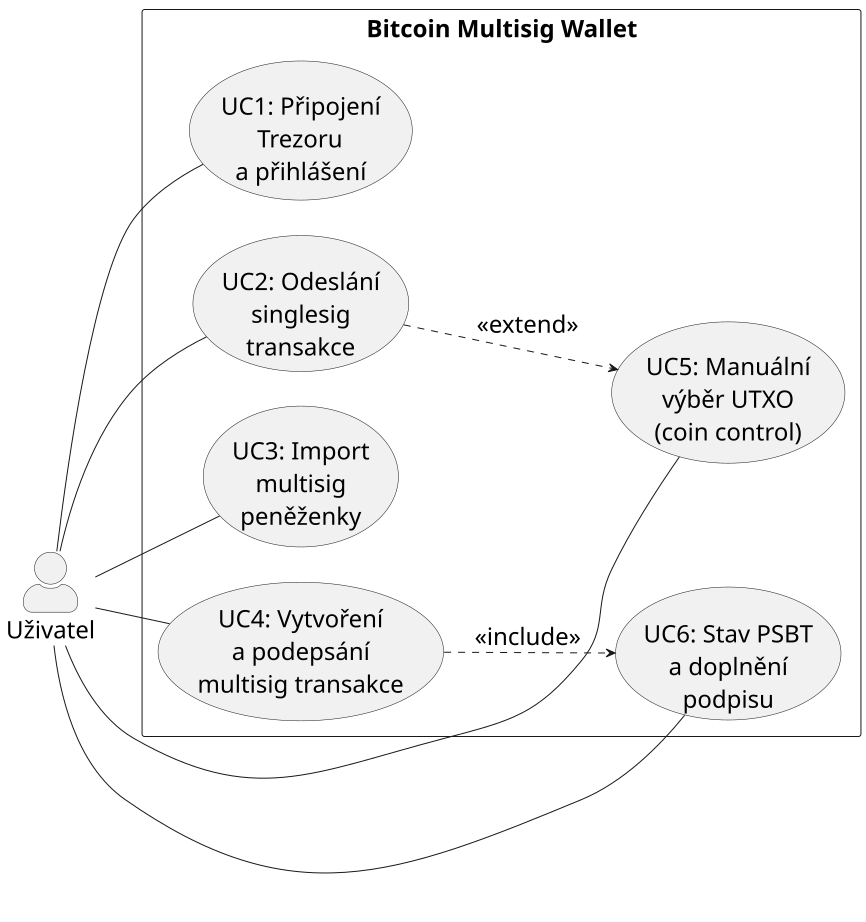
\includegraphics[width=\textwidth]{img/use-case.pdf}
\caption{Diagram případů užití. Uživatel interaguje se~systémem prostřednictvím
osmi hlavních funkcí; coin control rozšiřuje odeslání transakce a~přepnutí účtu
je součástí multisig podepisování.}
\label{fig:use-case}
\end{figure}

%%% -----------------------------------------------------------------------
\section{Funkční požadavky}
\label{sec:funkcni-pozadavky}

Funkční požadavky vycházejí z~výše uvedených user stories a~use cases.
Jsou rozděleny do tří oblastí; u~každého požadavku uvádíme vazbu na
příslušné US/UC.

\subsection{Autentizace a správa účtů}

\begin{description}
  \item[F1 -- Přihlášení přes Trezor \textnormal{(US1, UC1)}:]
    Systém umožní přihlášení prostřednictvím hardwarové peněženky Trezor
    s~využitím deeplink mechanismu (přesměrování do~jiné aplikace
    prostřednictvím speciální URL) Trezor Connect~\cite{TrezorConnect}.
    Při přihlášení aplikace vyžádá z~Trezoru deset rozšířených veřejných
    klíčů (xpub) pro derivační cesty tvaru \texttt{m/84'/c'/N'} dle
    BIP-84~\cite{BIP84}, kde \texttt{N} je v~rozsahu 0 až 9 a~\texttt{c}
    nabývá hodnoty 0 pro mainnet a~1 pro testnet.

  \item[F2 -- Discovery účtů \textnormal{(US1, UC1)}:]
    Backend pro každý přijatý xpub odvodí dávku adres podle BIP-44 gap
    limitu~\cite{BIP44} a~ověří na blockchainu, zda mají transakční
    historii. Pro účty s~nalezenou aktivitou automaticky vytvoří
    peněženky.

  \item[F3 -- Přepínání účtů \textnormal{(US10)}:]
    Systém umožní přepínání mezi singlesig a~multisig peněženkami
    prostřednictvím navigačního menu. Každý singlesig účet je hlavním
    účtem a~může mít přidružené multisig peněženky importované
    prostřednictvím deskriptorů.
\end{description}

\subsection{Singlesig transakce}

\begin{description}
  \item[F4 -- Zobrazení zůstatku \textnormal{(US2)}:]
    Systém zobrazí aktuální zůstatek peněženky v~BTC a~v~přepočtu na fiat
    měnu s~využitím směnného kurzu z~CoinGecko API~\cite{CoinGeckoAPI}.

  \item[F5 -- Odeslání prostředků \textnormal{(US3, UC2)}:]
    Systém umožní odeslání Bitcoinu na zadanou adresu (singlesig P2WPKH).
    Poplatek je vypočten deterministicky na základě počtu vstupů, výstupů
    a~uživatelem zvoleného fee rate (sat/vB).

  \item[F6 -- Příjem prostředků \textnormal{(US4)}:]
    Systém umožní příjem Bitcoinu zobrazením přijímací adresy a~QR kódu.

  \item[F7 -- Historie transakcí \textnormal{(US11)}:]
    Systém zobrazí historii transakcí včetně detailů (částka, adresa,
    poplatek, stav potvrzení).

  \item[F8 -- Coin control \textnormal{(US5, UC5)}:]
    Systém poskytne funkci manuálního výběru konkrétních UTXO jako vstupů
    transakce; poplatek je přepočítán při sestavení PSBT podle počtu
    vybraných vstupů.
\end{description}

\subsection{Multisignature transakce}

\begin{description}
  \item[F9 -- Import multisig peněženky \textnormal{(US6, UC3)}:]
    Systém umožní import multisig peněženky zadáním deskriptoru ve formátu
    \texttt{wsh(sortedmulti(\ldots))} dle BIP-380~\cite{BIP380}
    a~BIP-383~\cite{BIP383}. Deskriptor lze do aplikace dostat textovým
    vložením ze schránky nebo naskenováním QR kódu. Z~deskriptoru systém
    extrahuje práh M, veřejné klíče cosignerů a~derivační cesty dle
    BIP-48~\cite{BIP48}.

  \item[F10 -- Vytvoření PSBT \textnormal{(US7, UC4)}:]
    Systém umožní vytvoření částečně podepsané transakce ve formátu
    PSBT~\cite{BIP174} pro multisig peněženku. Veřejné klíče v~redeem
    skriptu jsou řazeny dle BIP-67~\cite{BIP67} na úrovni odvozených
    klíčů pro každý vstup.

  \item[F11 -- Podepsání PSBT \textnormal{(US7, US9, UC4, UC6)}:]
    Systém umožní podepsání PSBT prostřednictvím Trezoru s~derivační
    cestou odpovídající aktuálnímu cosignerovi.

  \item[F12 -- Stav PSBT \textnormal{(US8, UC6)}:]
    Systém zobrazí stav rozpracovaných PSBT -- počet shromážděných
    podpisů, chybějící cosigneři -- a~umožní doplnění podpisu dalším
    cosignerem.

  \item[F13 -- Broadcast transakce \textnormal{(UC4)}:]
    Po~dosažení prahu podpisů zmizí na~detailu PSBT tlačítko
    \emph{Sign with Trezor} a~místo něj se zobrazí \emph{Broadcast
    Transaction}. Po~jeho stisknutí aplikace zavolá broadcast
    endpoint a~finalizovanou transakci propaguje do~Bitcoin sítě.
    Broadcast je tedy explicitní akcí některého cosignera
    na~detailu PSBT -- po~přijetí posledního podpisu se transakce
    sama od~sebe neodesílá a~iniciuje ji vždy klient, nikoli
    server-side background úloha.
\end{description}

%%% -----------------------------------------------------------------------
\section{Nefunkční požadavky}
\label{sec:nefunkcni-pozadavky}

Nefunkční požadavky specifikují kvalitativní vlastnosti systému.

\subsection{Bezpečnost}

\begin{description}
  \item[NF1 -- Privátní klíče mimo server:]
    Server nikdy nedisponuje privátními klíči uživatele. Veškeré podepisování
    transakcí probíhá výhradně na hardwarové peněžence Trezor. Server pracuje
    pouze s~veřejnými klíči (xpub) a~nepodepsanými nebo částečně podepsanými
    transakcemi (PSBT).

  \item[NF2 -- Autentizace:]
    Komunikace mezi mobilní aplikací a~backendem je autentizována pomocí
    JWT tokenů (JSON Web Token -- digitálně podepsaný přístupový token
    nesoucí identitu zařízení). Token je vydán při přihlášení a~vázán
    na~deterministicky odvozený \texttt{deviceId} z~kořenového otisku
    Trezoru, takže opakovaná přihlášení ze~stejného zařízení vedou
    na~stejnou identitu.

  \item[NF3 -- Důvěryhodný síťový kanál:]
    Komunikace mezi aplikací a~backendem probíhá přes HTTP v~izolované
    LAN nebo ve~VPN (ve~vývojovém nasazení používáme Tailscale, které
    zajišťuje šifrování na~síťové vrstvě mezi zařízeními). TLS
    na~aplikační vrstvě není v~rámci této práce řešeno.
\end{description}

\subsection{Platforma a kompatibilita}

\begin{description}
  \item[NF4 -- Cílová platforma:]
    Mobilní aplikace je určena pro platformu Android s~minimální podporovanou
    verzí API~24 (Android~7.0) a~cílovou verzí API~34 (Android~14).

  \item[NF5 -- Hardwarová peněženka:]
    Systém vyžaduje hardwarovou peněženku Trezor řady Safe (modely Safe~3,
    Safe~5 nebo Safe~7; starší Trezor One není podporován) a~nainstalovanou
    aplikaci Trezor Suite Mobile, která slouží jako prostředník pro
    podepisování transakcí (podrobnou analýzu tohoto rozhodnutí
    a~zvažovaných alternativ uvádíme v~sekci~\ref{sec:analyza-trezor}).
    Peněženka se k~mobilnímu zařízení připojuje USB-C kabelem
    (Safe~3, Safe~5) nebo bezdrátově přes Bluetooth (pouze Safe~7).
\end{description}

\subsection{Použitelnost}

\begin{description}
  \item[NF6 -- Asynchronní operace:]
    Síťové operace (načítání zůstatku, broadcast transakce) probíhají asynchronně
    a~neblokují uživatelské rozhraní. Uživatel je o~probíhající operaci informován
    vizuálním indikátorem.
\end{description}

\subsection{Testovatelnost}

\begin{description}
  \item[NF7 -- Podpora testnetu:]
    Systém podporuje Bitcoin testnet4 (nejnovější testovací síť Bitcoinu,
    nástupce testnet3) pro účely vývoje a~testování bez rizika ztráty
    reálných prostředků. Trezor používá pro testnet stejné derivační cesty
    (\texttt{coin\_type = 1}) nezávisle na verzi testnetové sítě -- volba
    testnet4 se týká blockchainového API (Mempool.space). Přepínání
    mezi testnetem a~mainnetem provádí uživatel na přihlašovací obrazovce
    mobilní aplikace.
\end{description}

% Následující kapitoly budou doplněny v další verzi:
%%% Kapitola 3: Návrh

\chapter{Návrh}
\label{chap:navrh}

V~této kapitole představíme návrh architektury systému, zdůvodníme volbu
jednotlivých technologií a~popíšeme klíčová návrhová rozhodnutí. U~každého
rozhodnutí uvádíme, jaké alternativy jsme zvažovali a~proč jsme zvolili
právě daný přístup. Dále popíšeme bezpečnostní model, datový model,
workflow pro tvorbu a~podepisování transakcí a~návrh uživatelského rozhraní.

%% -----------------------------------------------------------------------
\section{Architektura systému}
\label{sec:architektura}

\subsection{Mikroservisní architektura}

Systém je navržen jako soustava šesti samostatných mikroslužeb, mobilní Android
aplikace a~společné API Gateway, která slouží jako jediný vstupní bod pro veškerou
komunikaci z~klientské aplikace. Každá mikroslužba má jasně vymezenou odpovědnost
a~vlastní datové úložiště (princip \emph{database per service}). Celkovou
architekturu zachycuje obrázek~\ref{fig:architektura}.

\begin{figure}[htbp]
\centering
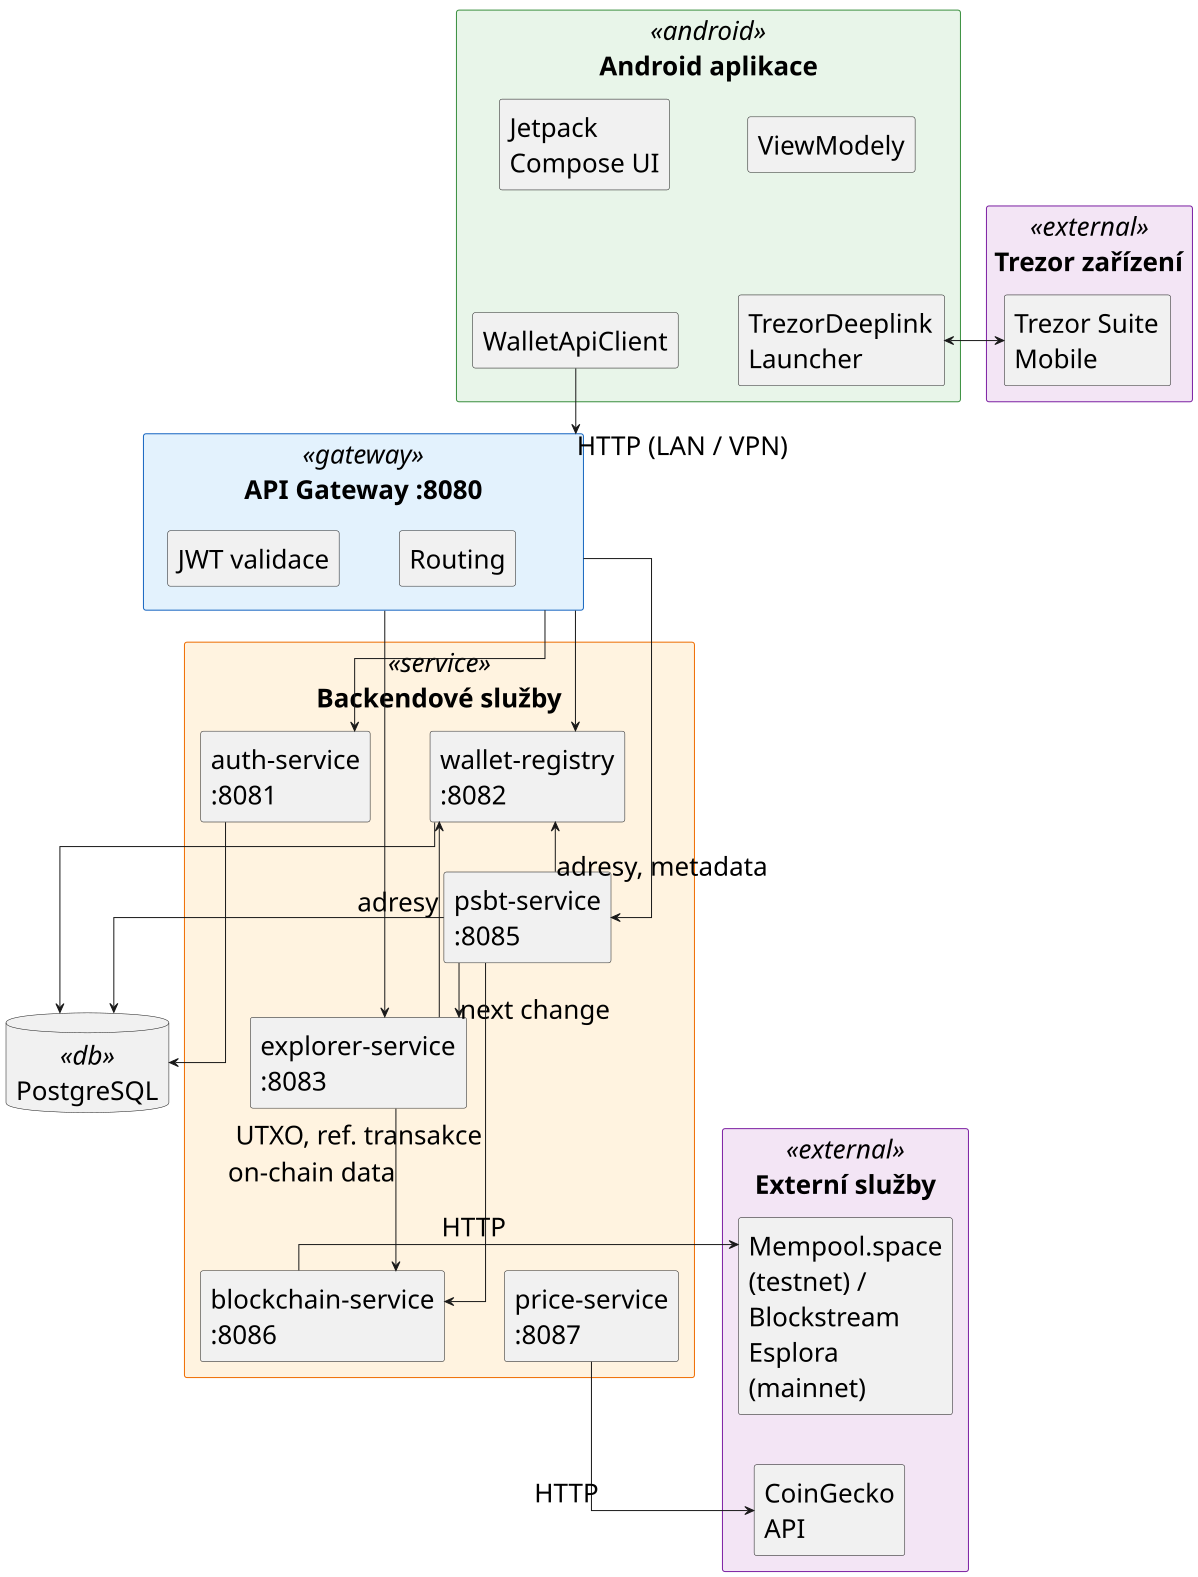
\includegraphics[width=\textwidth]{img/architektura.pdf}
\caption{Schéma architektury systému. Android aplikace komunikuje s~API
Gateway přes HTTP v~izolované LAN či VPN a~s~hardwarovou peněženkou
Trezor přes deeplink protokol zprostředkovaný aplikací Trezor Suite
Mobile. Backendové mikroslužby komunikují mezi sebou interně
a~přistupují k~externím službám (Mempool.space, CoinGecko).}
\label{fig:architektura}
\end{figure}

Při volbě architektonického stylu jsme zvažovali tři varianty:

\begin{description}
\item[Monolitická aplikace] -- jediný nasaditelný artefakt obsahující veškerou
  logiku. Výhodou je jednoduchost vývoje a~nasazení, nevýhodou pak rostoucí
  provázanost kódu a~nemožnost nezávislého škálování jednotlivých komponent.
  Pro peněženku s~vícero jasně oddělitelnými doménami (autentizace, správa peněženek,
  blockchain interakce, PSBT workflow) by monolitický přístup vedl
  k~nepřehledné kódové základně.

\item[Mikroservisy se sdílenou databází] -- služby jsou oddělené, ale sdílejí
  jedno databázové schéma. Tento kompromis usnadňuje dotazy napříč doménami,
  ale zavádí implicitní vazby mezi službami na úrovni datového modelu.
  Změna schématu jedné služby může nechtěně ovlivnit ostatní.

\item[Mikroservisy s~oddělenými databázemi] -- každá služba vlastní svá data
  a~komunikuje s~ostatními výhradně prostřednictvím definovaných API.
  Tento přístup jsme zvolili, protože poskytuje nejsilnější izolaci
  a~umožňuje nezávislý vývoj, nasazení i~škálování jednotlivých služeb.
\end{description}

Zvolili jsme třetí variantu. Systém využívá tři oddělené PostgreSQL~\cite{PostgreSQL} databáze:
jednu pro autentizaci a~správu zařízení (\texttt{auth-service}), jednu pro správu peněženek
a~adres (\texttt{wallet-registry}) a~jednu pro PSBT workflow
(\texttt{psbt-\allowbreak service}). Zbývající služby
(\texttt{explorer-\allowbreak service},
\texttt{blockchain-\allowbreak service},
\texttt{price-\allowbreak service}) jsou bezstavové a~žádnou vlastní
databázi nevyžadují -- slouží jako proxy k~externím API.

\subsection{API Gateway}

API Gateway běží na portu~8080 a~plní několik klíčových rolí:

\begin{itemize}
\item \textbf{Jednotný vstupní bod} -- klientská aplikace komunikuje výhradně
  s~jednou adresou a~nemusí znát topologii backendových služeb.
\item \textbf{Validace JWT tokenů} -- gateway ověřuje platnost přístupových
  tokenů algoritmem RS256 pomocí veřejného klíče získaného z~JWKS endpointu
  \texttt{auth-service}. Požadavky bez platného tokenu jsou odmítnuty
  s~kódem~401, aniž by se dostaly k~cílové službě.
\item \textbf{Směrování požadavků} -- na základě prefixu URL cesty gateway
  přeposílá požadavek na odpovídající mikroslužbu. Například prefix
  \texttt{/api/\allowbreak v1/\allowbreak wallets} je směrován převážně na
  \texttt{wallet-\allowbreak registry} (port~8082), prefix
  \texttt{/api/\allowbreak v1/\allowbreak psbt} na \texttt{psbt-\allowbreak service}
  (port~8085) a~podobně.
\item \textbf{Propagace identity} -- po úspěšné validaci tokenu gateway
  extrahuje identifikátor zařízení (\texttt{device\_id}) a~předává jej
  cílové službě jako query parametr nebo položku v~těle požadavku. Jednotlivé
  služby tak nemusí opakovaně validovat token a~mohou důvěřovat identitě
  předané gateway.
\end{itemize}

Alternativou k~vlastní implementaci gateway by bylo použití existujícího
řešení, například Kong, Traefik či Nginx s~Lua skripty. Zvažovali jsme
především Traefik pro jeho nativní integraci s~Dockerem~\cite{Docker}. Rozhodli jsme se
však pro vlastní implementaci v~Ktoru~\cite{KtorFramework}, protože požadavky na gateway jsou
relativně jednoduché (směrování, JWT validace) a~vlastní řešení umožnilo
sdílet kódovou základnu, datové třídy a~konfiguraci s~ostatními službami
bez nutnosti zavádět další technologii do stacku.

\subsection{Komunikace mezi službami}

Komunikace mezi API Gateway a~mikroslužbami probíhá synchronně prostřednictvím
HTTP požadavků. K~tomuto účelu využíváme Ktor~\cite{KtorFramework} \texttt{HttpClient} s~kotlinovými
korutinami, které zajišťují neblokující I/O operace.

Zvažovali jsme i~asynchronní komunikaci prostřednictvím fronty zpráv
(RabbitMQ, Apache Kafka). Tento přístup by byl vhodný pro systém s~vysokou
zátěží, kde je třeba oddělit producenta a~konzumenta zpráv. V~našem případě
však převažují synchronní operace typu požadavek--odpověď (dotaz na zůstatek,
vytvoření PSBT, podepsání transakce), pro které je HTTP přímočařejší
a~nevyžaduje provoz dalšího infrastrukturního komponentu. Navíc mobilní
klient přirozeně očekává okamžitou odpověď na svůj požadavek.

\subsection{Přehled mikroslužeb}

Systém se skládá z~následujících mikroslužeb:

\begin{description}
\item[\texttt{auth-service} (port 8081)] -- Zajišťuje autentizaci zařízení.
  Při prvním přihlášení vytvoří identitu zařízení na základě fingerprintu
  hardwarové peněženky Trezor a~vydá JWT přístupový token podepsaný algoritmem
  RS256. Token obsahuje \texttt{device\_id} jako \emph{subject} a~má omezenou
  platnost.

\item[\texttt{wallet-registry} (port~8082)] \hfill \\
  Spravuje peněženky, cosignery a~adresy. Pro singlesig peněženky provádí
  derivaci adres podle standardu BIP-32~\cite{BIP32} s~cestou
  \texttt{m/84'/\allowbreak 1'/\allowbreak 0'} (BIP-84~\cite{BIP84}).
  Pro multisig peněženky parsuje output deskriptory ve~formátu
  \texttt{wsh(\allowbreak sorted\-multi(...))} dle BIP-380~\cite{BIP380}
  a~BIP-383~\cite{BIP383} a~provádí derivaci P2WSH adres podle
  BIP-48~\cite{BIP48}.

\item[\texttt{explorer-service} (port 8083)] -- Agreguje data z~blockchainu
  pro konkrétní peněženku. Kombinuje informace o~zůstatku, historii transakcí
  a~nepoužitých výstupech (UTXO) získané z~\texttt{blockchain-service}
  s~adresami z~\texttt{wallet-registry}.

\item[\texttt{psbt-service} (port 8085)] -- Řídí celý životní cyklus PSBT
  transakcí: tvorbu, uložení, podepisování a~broadcast. Při vytváření PSBT
  sestaví parametry potřebné pro podepsání na zařízení Trezor
  prostřednictvím protokolu Trezor Connect~\cite{TrezorConnect}. Dosud
  nepoužitou change adresu pro každou novou transakci si vyžádá
  od~\texttt{explorer-service}; tím je zajištěno, že se~žádná change
  adresa v~čase neopakuje. Pro multisig peněženky sleduje počet
  sebraných podpisů a~umožňuje broadcast po dosažení požadovaného
  prahu~$M$.

\item[\texttt{blockchain-service} (port~8086)] \hfill \\
  Slouží jako proxy k~blockchainovému API. Na mainnetu využívá
  Blockstream Esplora, na testnet4 Mempool.space~\cite{MempoolAPI}
  (obě API sdílejí kompatibilní formát). Poskytuje zůstatky adres,
  seznamy UTXO, detaily transakcí a~aktuální odhady poplatků.

\item[\texttt{price-service} (port 8087)] -- Poskytuje aktuální směnný
  kurz Bitcoinu vůči fiat měnám. Data získává z~CoinGecko
  API~\cite{CoinGeckoAPI} a~kešuje je v~paměti s~krátkou dobou expirace,
  aby se minimalizoval počet externích volání.
\end{description}

%% -----------------------------------------------------------------------
\section{Volba technologií}
\label{sec:technologie}

V~této sekci zdůvodníme volbu konkrétních technologií. U~každé uvádíme, jaké
alternativy jsme zvažovali a~proč jsme se rozhodli právě pro danou variantu.

\subsection{Programovací jazyk: Kotlin}

Pro implementaci celého systému -- jak backendových služeb, tak mobilní
aplikace -- jsme zvolili jazyk Kotlin~\cite{KotlinLang}. Hlavní důvody byly:

\begin{itemize}
\item \textbf{Typová bezpečnost} -- Kotlin je staticky typovaný jazyk
  s~nulovatelností zakódovanou v~typovém systému (\emph{null safety}).
  Pro peněženku manipulující s~finančními prostředky je typová bezpečnost
  obzvláště důležitá, protože zabraňuje celé třídě chyb v~době kompilace.
\item \textbf{Korutiny} -- Kotlinové korutiny poskytují elegantní model
  pro asynchronní programování bez callback hell. Backendové služby zpracovávají
  mnoho souběžných HTTP požadavků a~korutiny umožňují psát neblokující kód
  sekvenčním stylem.
\item \textbf{Sdílený jazyk} -- Použití stejného jazyka pro backend i~frontend
  umožňuje sdílet datové třídy, validační logiku a~mentální model mezi oběma
  částmi systému. Vývojář nepotřebuje přepínat mezi různými jazyky a~jejich
  idiomy.
\item \textbf{Oficiální jazyk pro Android} -- Google označuje Kotlin jako
  preferovaný jazyk pro vývoj Android aplikací, což zaručuje dlouhodobou
  podporu a~rozsáhlý ekosystém knihoven.
\end{itemize}

Zvažovali jsme rovněž jazyk Dart (s~frameworkem Flutter) pro mobilní aplikaci
a~Go nebo TypeScript pro backend. Dart by umožnil multiplatformní vývoj
(Android i~iOS), avšak za cenu ztráty sdíleného jazyka s~backendem.
Bitcoinové knihovny pro Dart sice existují (např.\ \texttt{bitcoin\_flutter},
\texttt{dartsv}), ale jde o~menší komunitní projekty s~méně zralým ekosystémem
než JVM platforma s~knihovnou bitcoinj~\cite{BitcoinJ}. Go nabízí výborný výkon
a~jednoduchost a~disponuje kvalitními Bitcoinovými knihovnami (např.\ \texttt{btcd}),
ale postrádá vestavěnou podporu pro Android vývoj -- mobilní aplikaci
by bylo nutné řešit samostatně v~jiném jazyce, čímž by se ztratila výhoda
sdíleného kódu.

\subsection{Backend framework: Ktor}

\begin{sloppypar}
Pro implementaci backendových služeb jsme zvolili framework
Ktor \cite{KtorFramework}. Alternativou byl především Spring Boot,
nejpoužívanější framework pro JVM back\-endy. Ktor jsme upřednostnili
z~následujících důvodů:
\end{sloppypar}

\begin{itemize}
\item \textbf{Nativní podpora korutin} -- Ktor je od základu navržen
  s~kotlinovými korutinami. Každý příchozí požadavek je zpracován v~korutině,
  což umožňuje neblokující obsluhu tisíců souběžných spojení s~minimální
  paměťovou náročností.
\item \textbf{Minimalistický design} -- Ktor nepřidává žádnou \uv{magii} --
  nepoužívá reflexi, anotační procesory ani dependency injection kontejner.
  Konfigurace probíhá explicitně v~kódu, což zvyšuje čitelnost
  a~předvídatelnost chování.
\item \textbf{Modulární architektura} -- Funkcionalita se přidává formou
  pluginů (autentizace, serializace, CORS, logování). Výsledný artefakt
  obsahuje pouze skutečně používané komponenty.
\item \textbf{Nízká paměťová náročnost} -- Mikroslužby nasazujeme v~Docker
  kontejnerech a~pro provoz peněženky s~řádově jednotkami až desítkami
  uživatelů nepotřebujeme těžký aplikační framework. Ktor služba startuje
  v~řádu stovek milisekund a~spotřebuje výrazně méně paměti než srovnatelná
  Spring Boot aplikace.
\end{itemize}

Spring Boot by nabídl robustnější ekosystém (Spring Security, Spring Data),
ale pro naše účely by představoval zbytečnou složitost. Naše služby mají
úzce vymezené API s~řádově jednotkami endpointů a~nepotřebují pokročilé
funkce jako ORM nebo deklarativní security pravidla.

\subsection{Mobilní framework: Jetpack Compose}

\begin{sloppypar}
Pro uživatelské rozhraní mobilní aplikace jsme zvolili Jetpack
Compose \cite{JetpackCompose}, moderní deklarativní UI toolkit
od~Googlu. Alternativou byl klasický přístup pomocí XML layout
souborů a~View systému.
\end{sloppypar}

Jetpack Compose jsme zvolili z~následujících důvodů:

\begin{itemize}
\item \textbf{Deklarativní paradigma} -- UI se popisuje jako funkce stavu.
  Při změně stavu se automaticky překreslí pouze dotčené části, bez nutnosti
  manuální manipulace s~View objekty. To vede k~méně chybovému a~lépe
  testovatelnému kódu.
\item \textbf{Méně boilerplate kódu} -- Odpadá nutnost definovat
  XML layouty, View\-Holdery, Adaptery a~další ceremoniální kód
  typický pro starší Android přístup. UI komponenty se píší přímo
  v~Kotlinu.
\item \textbf{Budoucí standard} -- Google aktivně doporučuje Jetpack Compose
  jako preferovaný způsob tvorby Android UI a~investuje do jeho rozvoje.
  Nové Android API se primárně navrhují s~ohledem na Compose.
\item \textbf{Integrace s~Kotlinem} -- Compose přirozeně využívá Kotlinové
  jazykové konstrukce (lambda výrazy, extension funkce, korutiny), což vede
  ke konzistentnímu a~idiomatickému kódu.
\end{itemize}

\subsection{Databáze: PostgreSQL}

Jako databázový systém jsme zvolili PostgreSQL~\cite{PostgreSQL}. Zvažovali
jsme rovněž SQLite (vestavěnou přímo v~mobilní aplikaci) a~MySQL/MariaDB.

PostgreSQL jsme upřednostnili z~následujících důvodů:

\begin{itemize}
\item \textbf{Silná konzistence a~ACID} -- Pro systém pracující s~finančními
  transakcemi je zásadní, aby databázové operace byly atomické a~konzistentní.
  Například při ukládání podpisu k~PSBT je nutné atomicky inkrementovat
  počítadlo podpisů a~ověřit dosažení prahu.
\item \textbf{Souběžné zápisy z~více služeb} -- v~mikroservisní architektuře
  do téže databáze paralelně píše více služeb i~několik instancí téže
  služby. Postgres MVCC zajišťuje korektní izolaci souběžných transakcí
  bez nutnosti aplikačního zamykání.
\item \textbf{Zralost a~rozšířenost} -- PostgreSQL je jeden z~nejrozšířenějších
  open-source databázových systémů s~rozsáhlou dokumentací a~komunitou.
\end{itemize}

SQLite by bylo vhodné řešení pro čistě mobilní aplikaci bez backendu, ale
v~zvolené architektuře databáze běží na serveru a~je sdílena mezi požadavky
od různých zařízení. MySQL by bylo funkčně rovnocenné pro většinu operací;
PostgreSQL jsme upřednostnili pro robustnější MVCC izolaci souběžných
transakcí a~širší ekosystém nástrojů (Flyway migrace, Exposed ORM).

\subsection{Kontejnerizace: Docker Compose}

Pro nasazení a~orchestraci všech backendových služeb používáme Docker
Compose~\cite{Docker}. Každá mikroslužba, API Gateway a~databázové instance
běží ve vlastním kontejneru. Zvažovali jsme i~Kubernetes, který by umožnil
pokročilé škálování a~self-healing, ale pro vývoj a~provoz peněženky
s~omezeným počtem uživatelů je Kubernetes zbytečně komplexní. Docker Compose
plně postačuje a~umožňuje jedním příkazem (\texttt{docker compose up})
spustit celý systém včetně databází, migrací a~všech služeb.

Hlavní výhody kontejnerizace v~kontextu tohoto systému:

\begin{itemize}
\item \textbf{Reprodukovatelné prostředí} -- vývojové, testovací a~produkční
  prostředí je identické, čímž se eliminují problémy typu \uv{u~mě to funguje}.
\item \textbf{Izolace služeb} -- každá služba běží ve vlastním kontejneru
  se svými závislostmi. Aktualizace jedné služby neovlivní ostatní.
\item \textbf{Definovaná síťová topologie} -- Docker Compose vytváří interní
  síť, kde se služby navzájem adresují jménem kontejneru. Mobilní aplikace
  komunikuje pouze s~gateway, ostatní služby nejsou z~vnějšku dostupné.
\end{itemize}

\subsection{Blockchainové API}

Pro získávání dat z~Bitcoin blockchainu (zůstatky adres, seznamy UTXO,
detaily transakcí, odhady poplatků) jsme zvažovali tři varianty:

\begin{itemize}
\item \textbf{Vlastní Bitcoin full node} -- poskytuje maximální nezávislost
  a~soukromí, ale vyžaduje stovky gigabajtů diskového prostoru a~kontinuální
  synchronizaci s~sítí. Pro testovací a~vývojové účely je toto nepraktické.
\item \textbf{Blockstream Esplora API}~\cite{BlockstreamEsplora} -- open-source
  řešení s~veřejným REST API a~tolerantními rate limity. Nepodporuje však síť testnet4
  (novější testovací síť Bitcoinu), která je potřebná pro vývoj.
\item \textbf{Mempool.space API} -- rovněž open-source, s~plnou podporou
  testnet4, bez nutnosti API klíče. Poskytuje kvalitní odhady poplatků
  na základě aktuálního stavu mempoolu. Oproti Blockstream Esplora má
  však přísnější rate limity.
\end{itemize}

Obě služby (Blockstream Esplora i~Mempool.space) sdílejí kompatibilní
REST API formát, což umožňuje použít stejnou klientskou implementaci
pro obě. Využíváme proto obě: na mainnetu Blockstream Esplora~\cite{BlockstreamEsplora}
(\url{https://blockstream.info/api}) pro jeho stabilitu a~tolerantní
rate limity, na testnet4 Mempool.space
(\url{https://mempool.space/testnet4/api}), protože Blockstream Esplora
testnet4 nepodporuje. Aktivní poskytovatel se volí podle konfigurace sítě.

Díky izolaci blockchainové komunikace do samostatné služby
\texttt{blockchain-\allowbreak service} je možné poskytovatele snadno
zaměnit nebo přidat podporu vlastního full node bez zásahu do zbytku systému.

\subsection{Cenový zdroj: CoinGecko API}

Pro zobrazení aktuální hodnoty prostředků ve fiat měně používáme
CoinGecko API~\cite{CoinGeckoAPI}. CoinGecko nabízí bezplatný tier
s~dostatečným limitem požadavků (30~volání za minutu na Demo API
klíči), podporuje desítky fiat měn a~vyžaduje pouze bezplatnou
registraci. Alternativou by bylo CoinMarketCap API, které pro
bezplatný plán nabízí méně velkorysé limity.

%% -----------------------------------------------------------------------
\section{Bezpečnostní model}
\label{sec:bezpecnost}

Bezpečnostní model aplikace je postaven na fundamentálním principu:
\textbf{server nikdy nedisponuje privátními klíči uživatele}. Veškeré
kryptografické operace spojené s~podepisováním transakcí probíhají výhradně
na hardwarovém zařízení Trezor, které nikdy neopustí fyzický dosah uživatele.
I~v~případě kompletní kompromitace serveru tak útočník nezíská prostředky
k~odcizení Bitcoinů.

\subsection{Autentizace a identita}

Pro autentizaci zařízení používáme JWT (\emph{JSON Web Token}) tokeny
podepsané asymetrickým algoritmem RS256. Schéma autentizace funguje
následovně:

\begin{enumerate}
\item Uživatel připojí hardwarovou peněženku Trezor k~mobilnímu zařízení.
\item Aplikace prostřednictvím Trezor Connect získá veřejné informace
  o~zařízení -- především \emph{fingerprint} kořenového veřejného klíče.
\item Z~fingerprintu je deterministicky odvozen \texttt{device\_id}
  (UUID verze~3 s~prefixem \texttt{trezor:}).
\item \texttt{auth-service} uloží identitu zařízení a~vydá JWT token
  podepsaný svým privátním RSA klíčem. Token obsahuje \texttt{device\_id}
  jako \emph{subject} a~má omezenou dobu platnosti.
\item API Gateway validuje token při každém požadavku pomocí veřejného
  klíče získaného z~JWKS endpointu \texttt{auth-service}.
\end{enumerate}

Celý průběh autentizace zachycuje obrázek~\ref{fig:auth-flow}.

\begin{figure}[htbp]
\centering
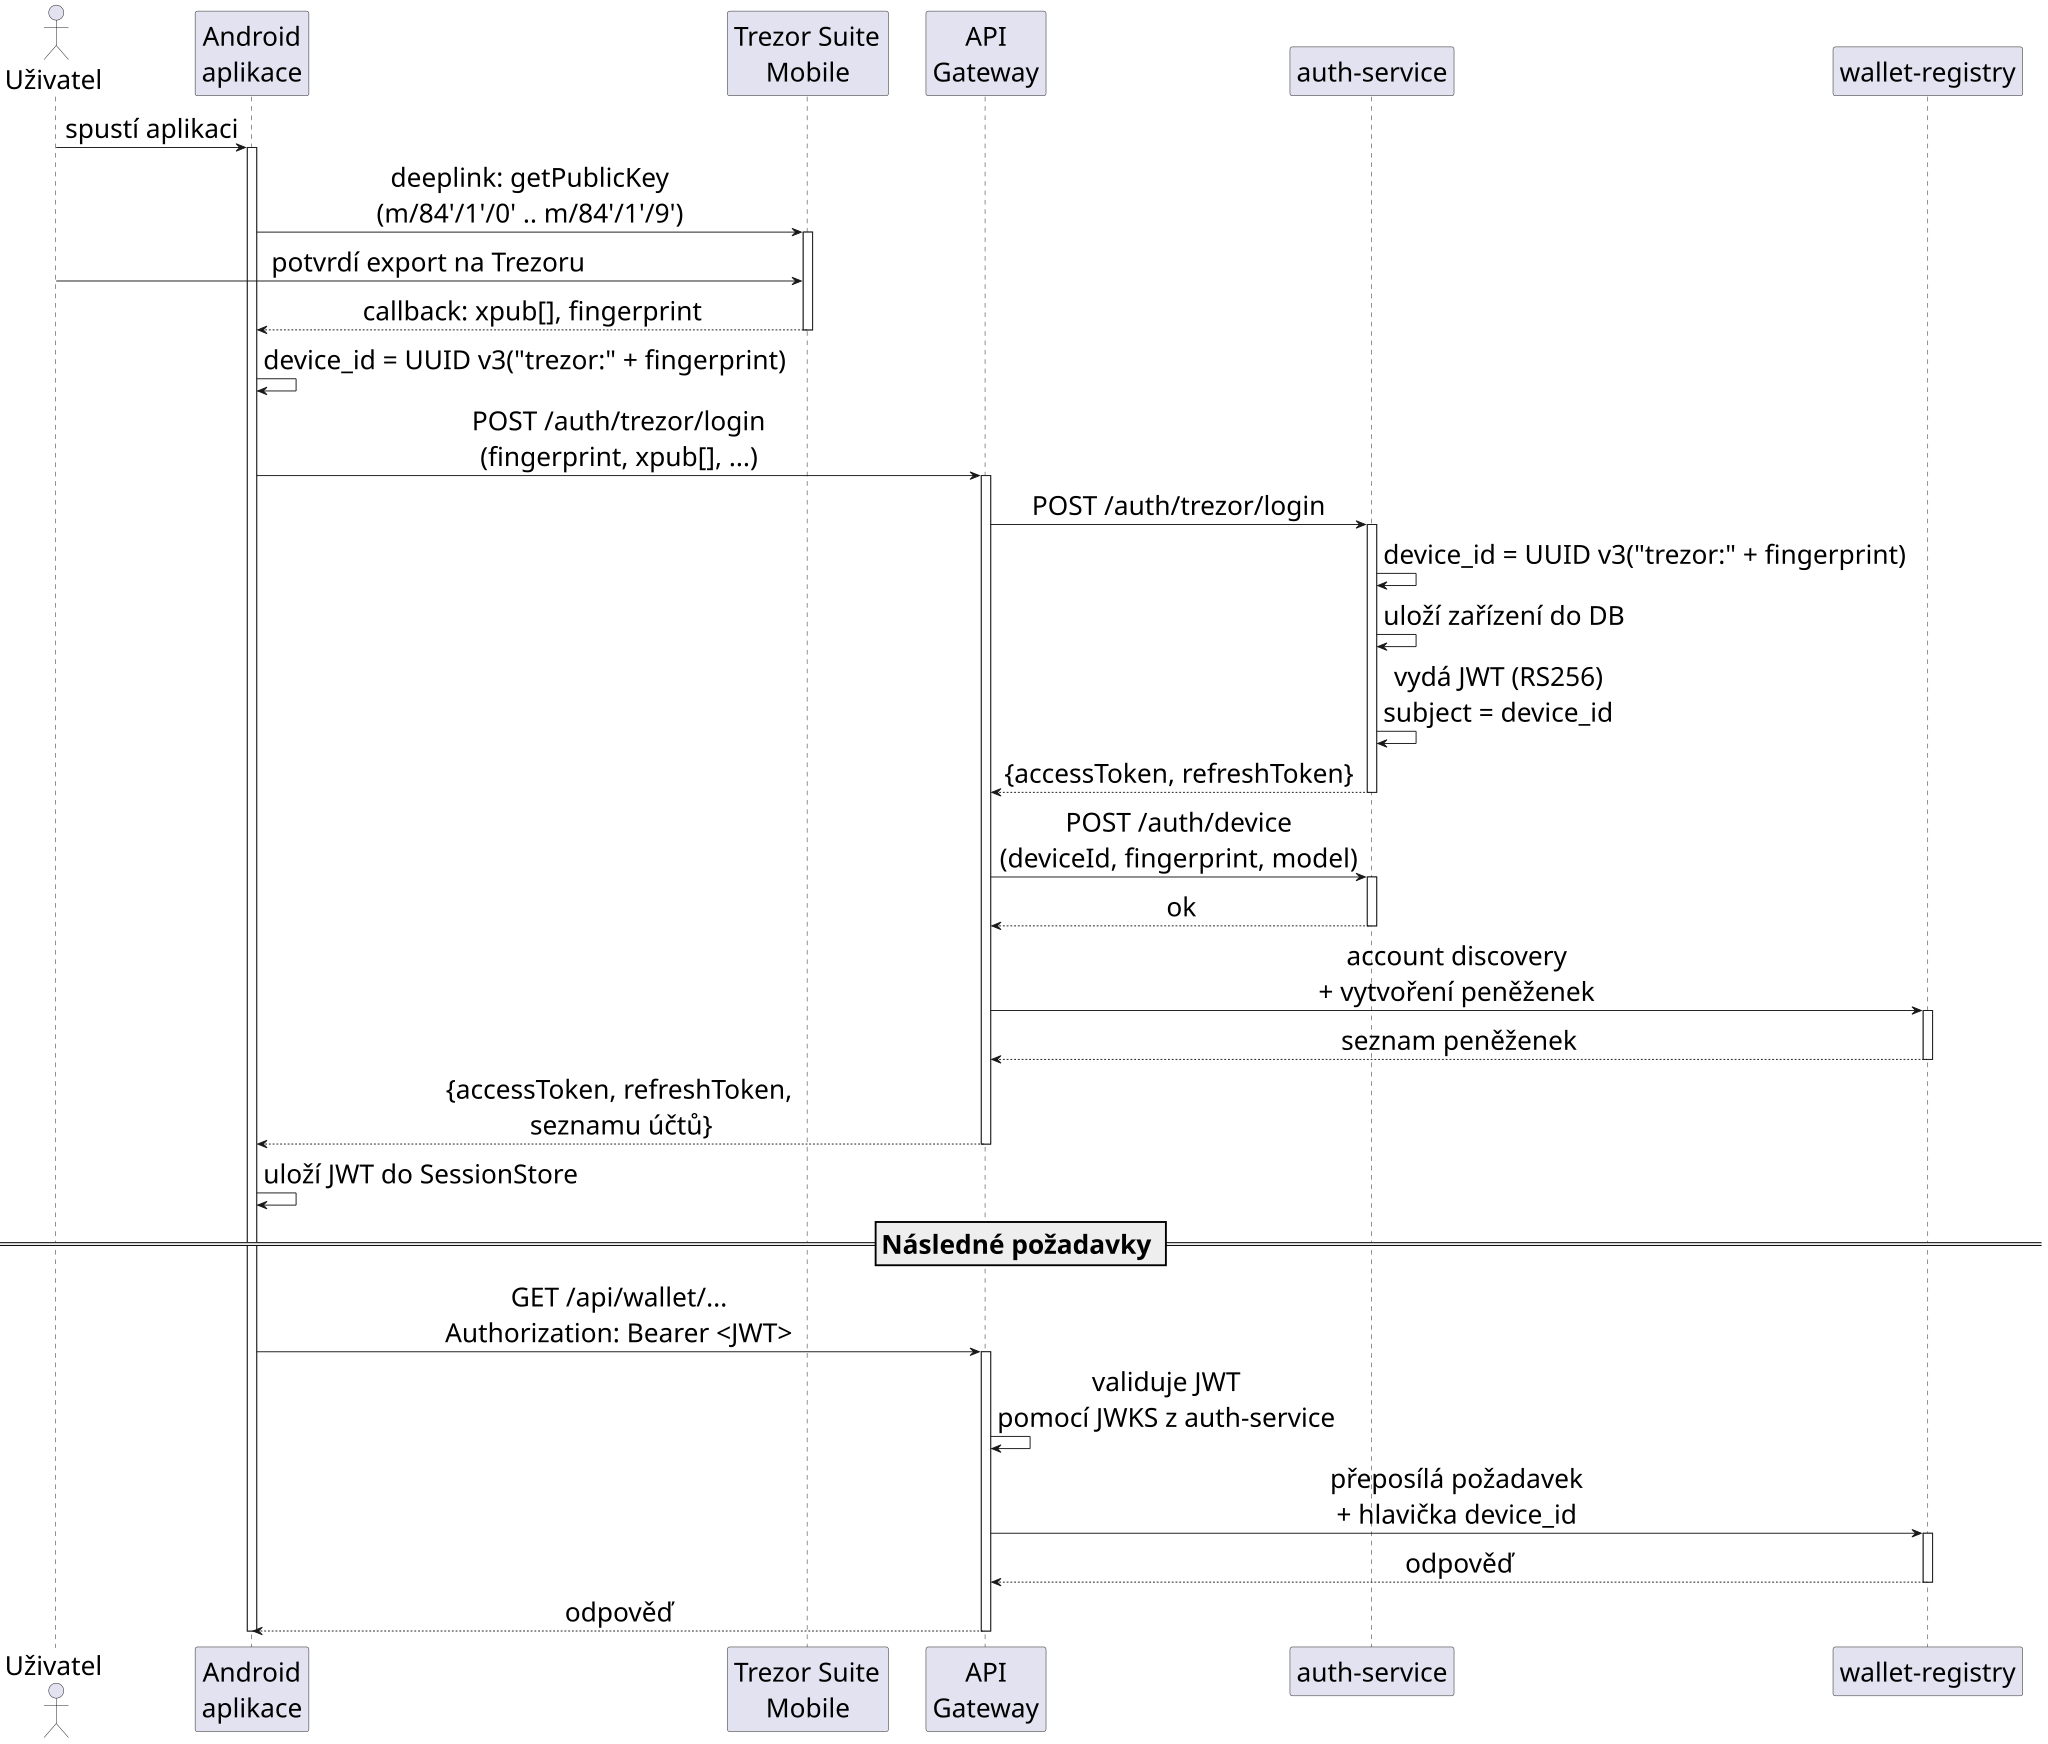
\includegraphics[width=\textwidth,height=0.85\textheight,keepaspectratio]{img/auth-flow.pdf}
\caption{Sekvenční diagram autentizace. Uživatel exportuje veřejné klíče
z~Trezoru přes Trezor Suite Mobile, \texttt{auth-service} uloží zařízení
a~vydá JWT token, API Gateway následně validuje token při každém požadavku.}
\label{fig:auth-flow}
\end{figure}

Zvažovali jsme i~jednodušší autentizační schémata -- například symetrické
HMAC tokeny nebo statické API klíče. Asymetrický RS256 jsme zvolili proto,
že umožňuje distribuci veřejného klíče přes JWKS endpoint: gateway i~ostatní
služby mohou nezávisle ověřovat tokeny, aniž by sdílely tajný klíč
s~\texttt{auth-service}. To snižuje plochu útoku -- kompromitace gateway
neumožní vystavovat falešné tokeny.

Identita zařízení je odvozena z~fingerprintu Trezoru, nikoliv z~uživatelského
jména a~hesla. Tento přístup reflektuje specifika aplikace: uživatel
se neidentifikuje svou osobou, ale svým hardwarovým zařízením. Zároveň
tak odpadá nutnost spravovat hesla, řešit jejich reset a~chránit je
před únikem.

\subsubsection{Obnova přístupového tokenu přes refresh token}
\label{subsec:refresh-token}

Přístupový JWT token má platnost 24~hodin. Bez dalšího mechanismu by
uživatel musel po~každém vypršení znovu exportovat veřejné klíče
z~Trezoru, což by výrazně zhoršilo uživatelský komfort -- uživatel
by přitom neměnil identitu, pouze obnovoval relaci. Proto \texttt{auth-service}
při~přihlášení vydá vedle přístupového tokenu ještě tzv.~\emph{refresh
token} s~delší platností (30~dní), který aplikace uchová spolu
s~přístupovým tokenem a~použije jej k~obnově, jakmile přístupový token
vyprší.

Refresh tokeny jsou navrženy jako \emph{jednorázové} -- každý token
lze použít pouze k~jediné výměně za~novou dvojici. Rotace probíhá takto:

\begin{enumerate}
\item Aplikace pošle aktuální refresh token na \texttt{POST /auth/token/refresh}.
\item \texttt{auth-service} v~jedné databázové transakci vyhledá záznam
  podle hashe tokenu, ověří, že není expirovaný ani dříve revokovaný,
  atomicky nastaví sloupec \texttt{revoked\_at} a~vydá novou dvojici
  (přístupový $+$ refresh token).
\item Aplikace nové tokeny uloží do~perzistence a~starý refresh token
  už znovu nepoužije.
\end{enumerate}

Krok~2 je race-safe: klauzule \texttt{UPDATE \ldots WHERE revoked\_at
IS NULL} zajišťuje, že pokud stejný refresh token dorazí na~server
souběžně dvakrát, vyhraje pouze jeden \texttt{UPDATE}; druhý uvidí
nulový počet aktualizovaných řádků a~vrátí klientovi~401. Tím se brání
situaci, kdy by dvě souběžné výměny vygenerovaly dva platné refresh
tokeny ze~stejného originálu.

V~databázi je uložen pouze SHA-256 hash tokenu, nikoli jeho otevřená
hodnota. Případný únik obsahu tabulky \texttt{refresh\_tokens} tedy
neumožní útočníkovi používat aktivní tokeny -- získá pouze otisky,
ze~kterých původní hodnotu nelze zpětně odvodit. Otevřená hodnota
existuje výhradně v~paměti klienta a~v~jeho lokálním perzistentním
úložišti.

\subsection{Absence privátních klíčů na serveru}

Na serveru nejsou uloženy žádné privátní klíče, seed fráze ani jakékoliv
materiály, z~nichž by bylo možné privátní klíče odvodit. Server disponuje
pouze veřejnými klíči (xpub) potřebnými pro derivaci adres a~ověřování
podpisů. Toto oddělení je zásadní pro bezpečnostní model aplikace --
i~v~případě úplné kompromitace serveru útočník získá pouze veřejné informace
(adresy, zůstatky, historii transakcí), nikoliv prostředky k~odcizení
prostředků.

\subsection{Podepisování transakcí přes Trezor Connect}
\label{subsec:trezor-connect}

Jak jsme analyzovali v~sekci~\ref{sec:analyza-trezor}, podepisování
transakcí probíhá prostřednictvím deeplink protokolu Trezor
Connect~\cite{TrezorConnect} s~aplikací Trezor Suite Mobile jako
prostředníkem. Konkrétní průběh podepisování:

\begin{enumerate}
\item Backend (\texttt{psbt-service}) sestaví z~PSBT transakce parametry
  ve formátu požadovaném Trezor Connect (vstupy s~derivačními cestami,
  výstupy s~adresami a~částkami).
\item Mobilní aplikace obdrží tyto parametry a~otevře Trezor Suite Mobile
  prostřednictvím deeplinku Trezor Connect
  (\texttt{https://\allowbreak connect.\allowbreak trezor.\allowbreak io/\allowbreak 9/\allowbreak deeplink/\allowbreak 1/}).
\item Uživatel ověří detaily transakce na displeji hardwarové peněženky
  a~potvrdí podpis fyzickým stisknutím tlačítka.
\item Trezor Suite Mobile vrátí výsledek zpět do aplikace prostřednictvím
  callback deeplinku.
\item Trezor Connect vždy vrací jak \texttt{serializedTx}, tak pole
  \texttt{signatures}. V~případě singlesig peněženky aplikace použije
  serializovanou transakci přímo k~broadcastu. V~případě multisig peněženky
  aplikace extrahuje pole podpisů a~odešle je na backend, který je přidá
  k~PSBT a~zkontroluje, zda byl dosažen požadovaný práh~$M$.
\end{enumerate}

Tento mechanismus zajišťuje, že privátní klíč nikdy neopustí bezpečné
prostředí hardwarové peněženky. Uživatel má plnou kontrolu nad tím, jaké
transakce podepisuje, protože detaily vždy ověřuje přímo na zařízení Trezor.

Kromě podepisování transakcí využíváme Trezor Connect i~pro \textbf{ověření
přijímací adresy na zařízení}. Při příjmu prostředků může uživatel stisknout
tlačítko \emph{Zobrazit na Trezoru}, čímž aplikace prostřednictvím deeplinku
zavolá metodu \texttt{getAddress} s~parametrem \texttt{showOnTrezor: true}.
Trezor na svém displeji zobrazí adresu odvozenou přímo z~klíčů uložených
v~zařízení a~uživatel ji může vizuálně porovnat s~adresou zobrazenou
v~aplikaci. Tím se eliminuje riziko, že by kompromitovaná aplikace nebo
server podvrhly cizí adresu -- útočník by musel současně ovládnout
i~firmware hardwarové peněženky, což je prakticky nemožné. Pro multisig
peněženky parametry volání zahrnují veřejné klíče všech cosignerů seřazené
podle BIP-67~\cite{BIP67}, aby Trezor mohl nezávisle odvodit správnou
P2WSH adresu.

Celý průběh podepisování zachycují obrázky~\ref{fig:trezor-signing-1}
a~\ref{fig:trezor-signing-2}.

\begin{figure}[htbp]
\centering
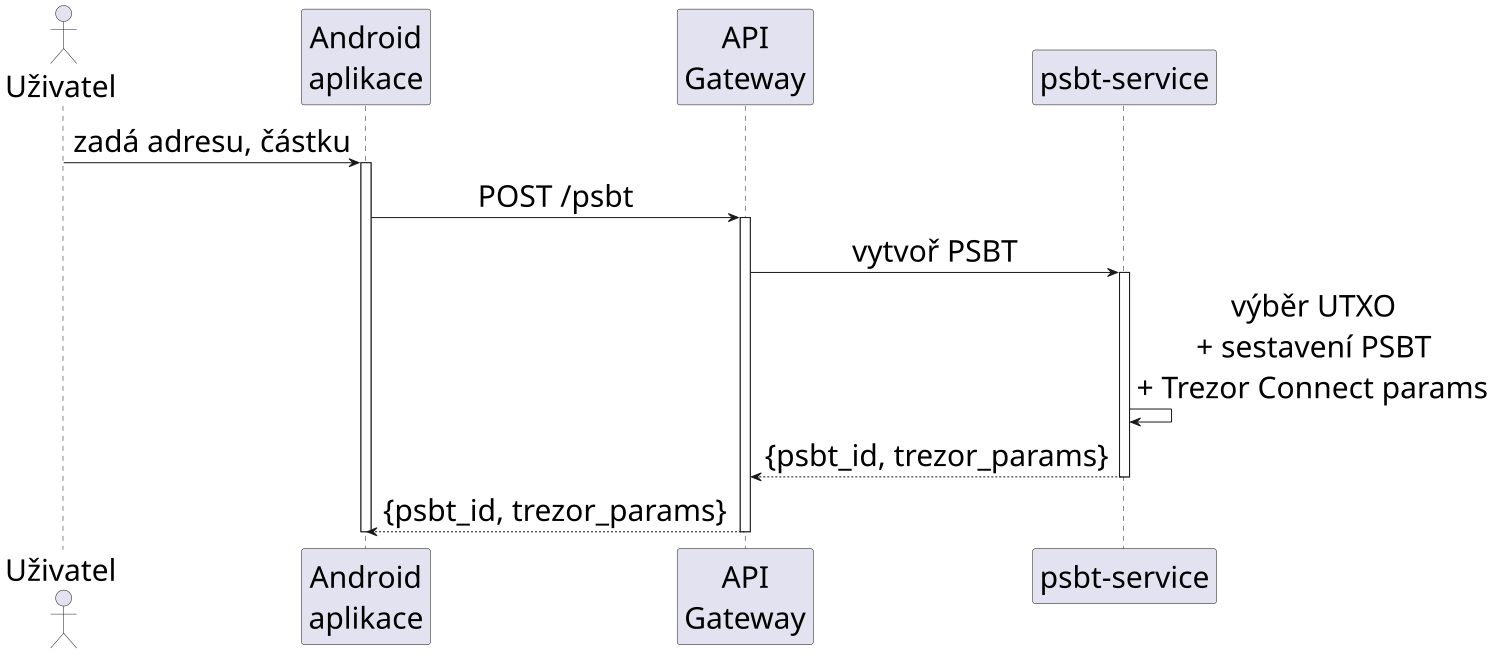
\includegraphics[width=\textwidth]{img/trezor-signing-1.pdf}
\caption{Sekvenční diagram podepisování -- první část: vytvoření PSBT na
backendu. Aplikace zadá požadavek API Gateway, \texttt{psbt-service}
vybere UTXO, sestaví PSBT a~připraví parametry pro Trezor Connect.}
\label{fig:trezor-signing-1}
\end{figure}

V~první fázi backend sestaví částečně podepsanou transakci ve~formátu
BIP-174. Pro multisig peněženku PSBT obsahuje kromě nepodepsané
transakce i~kompletní witness skript, derivační cesty všech cosignerů
a~předchozí transakce referencovaných UTXO -- vše, co Trezor potřebuje
k~ověření před podpisem. Spolu s~PSBT backend vrací strukturovaný
JSON objekt s~parametry pro Trezor Connect, který přesně odpovídá
formátu očekávanému metodou \texttt{signTransaction}.

V~druhé fázi mobilní aplikace předá tyto parametry Trezor Suite Mobile
a~uživatel transakci podepíše na hardwarovém zařízení. Návrat do aplikace
se liší podle typu peněženky: pro singlesig Trezor vrátí kompletní
serializovanou transakci, kterou aplikace pošle k~broadcastu; pro multisig
vrací pouze pole podpisů, které backend přidá do PSBT na pozici
odpovídající aktuálnímu cosignerovi.

\begin{figure}[htbp]
\centering
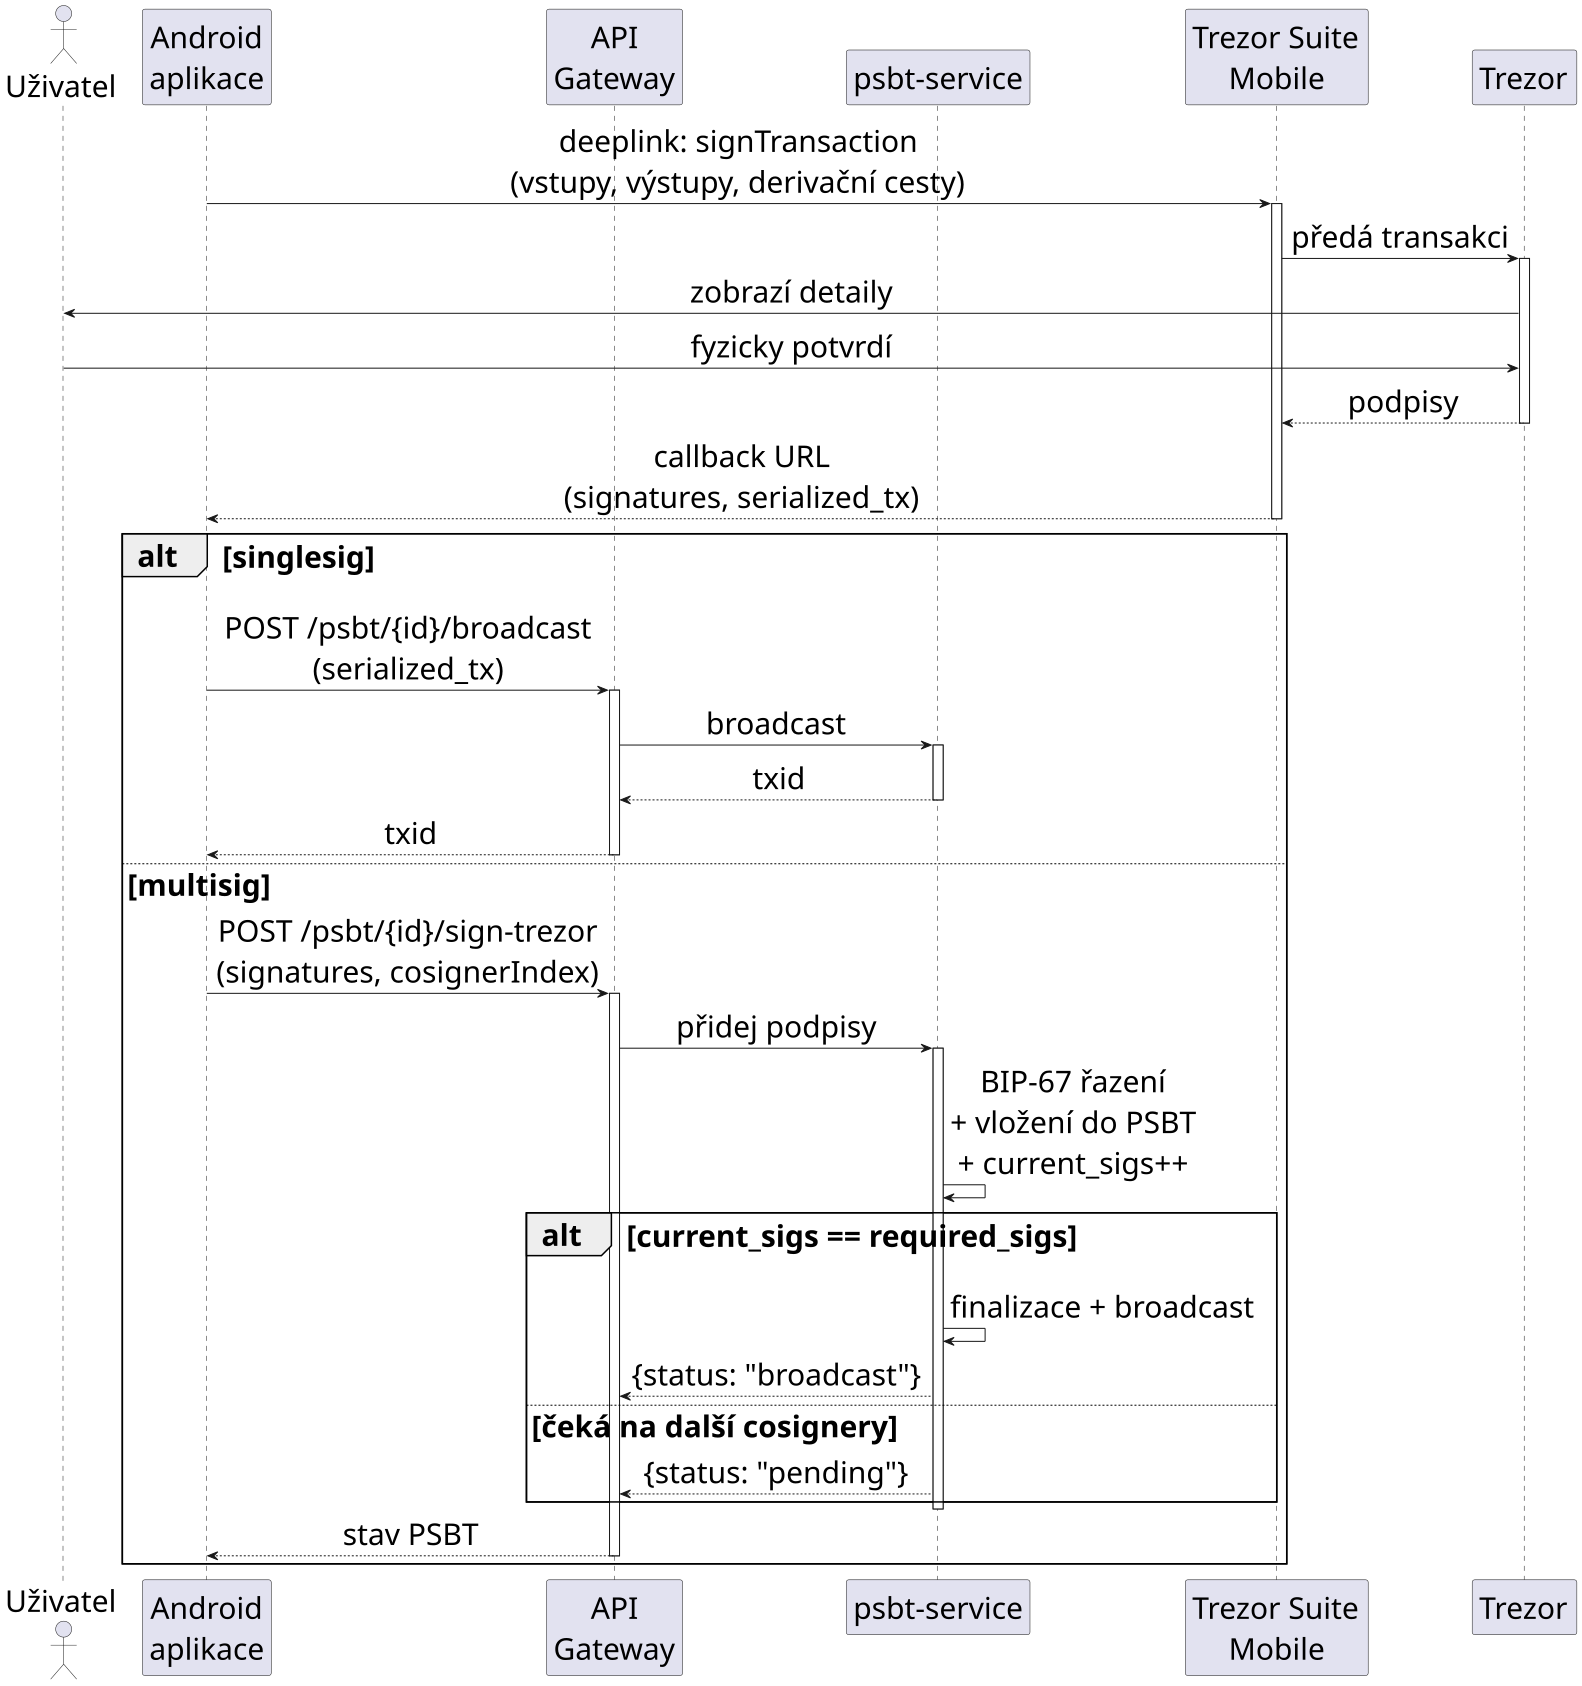
\includegraphics[width=\textwidth]{img/trezor-signing-2.pdf}
\caption{Sekvenční diagram podepisování -- druhá část: podpis na hardwarovém
zařízení a~následný broadcast (singlesig) nebo přidání dílčího podpisu
(multisig). Detaily transakce uživatel vždy ověřuje přímo na displeji
Trezoru.}
\label{fig:trezor-signing-2}
\end{figure}

%% -----------------------------------------------------------------------
\section{Datový model}
\label{sec:datovy-model}

Datový model systému je rozdělen do tří databází odpovídajících mikroslužbám,
které potřebují perzistentní úložiště. V~této sekci popíšeme hlavní entity
a~jejich vztahy.

\subsection{Databáze autentizační služby}

Databáze \texttt{auth-service} obsahuje dvě tabulky:

\begin{description}
\item[\texttt{devices}] -- Uchovává identitu autentizovaných zařízení.
  Primárním klíčem je \texttt{device\_id} (UUID odvozený z~fingerprintu).
  Dále obsahuje \texttt{fingerprint} kořenového veřejného klíče Trezoru,
  \texttt{model} (typ zařízení) a~\texttt{label} (uživatelský název).

\item[\texttt{refresh\_tokens}] -- Persistentní úložiště refresh tokenů
  s~jednorázovou rotací. Primárním klíčem je SHA-256 hash tokenu
  (otevřená hodnota se v~databázi nikdy neukládá, viz
  sekci~\ref{subsec:refresh-token}). Dále obsahuje
  \texttt{device\_\allowbreak id} (zařízení, kterému token patří),
  \texttt{fingerprint} kořenového klíče,
  \texttt{expires\_\allowbreak at} (platnost, default 30~dní),
  \texttt{created\_\allowbreak at} (vystavení) a~\texttt{revoked\_\allowbreak at}
  (čas revokace, \texttt{NULL} značí dosud platný token). Sloupec
  \texttt{revoked\_\allowbreak at} je load-bearing pro race-safe rotaci
  popsanou v~sekci~\ref{subsec:refresh-token}.
\end{description}

\subsection{Databáze wallet-registry}

Databáze \texttt{wallet-registry} obsahuje entity pro správu peněženek,
cosignerů a~adres:

\begin{description}
\item[\texttt{wallets}] {\sloppy -- Reprezentuje peněženku
  (singlesig nebo multisig). Identifikátor
  \texttt{wallet\_\allowbreak id} je deterministicky generován:
  u~multisig peněženek jako zkrácený SHA-256 hash output deskriptoru
  (s~prefixem sítě), u~singlesig jako kompozitní klíč
  \texttt{wallet-\{fingerprint\}-\{network\}-\{scriptType\}-\{accountIndex\}}.
  Oba přístupy zajišťují, že totožná peněženka vždy vede ke~stejnému
  identifikátoru. Tabulka dále obsahuje
  \texttt{network} (mainnet/\allowbreak testnet),
  \texttt{type} (SINGLE\_\allowbreak SIG~/~MULTI\_\allowbreak SIG),
  \texttt{script\_\allowbreak type} (P2WPKH~/~P2WSH), požadovaný
  počet podpisů~$M$, celkový počet cosignerů~$N$ a~dva kompletní
  deskriptory (\texttt{receive\_\allowbreak descriptor} pro přijímací
  adresy a~\texttt{change\_\allowbreak descriptor} pro change
  adresy).\par}

\item[\texttt{cosigners}] -- Uchovává veřejné klíče (xpub) jednotlivých
  cosignerů. Každý záznam obsahuje \texttt{fingerprint} nadřazeného klíče,
  \texttt{origin\_path} (derivační cesta, například \texttt{48'/1'/0'/2'})
  a~samotný rozšířený veřejný klíč \texttt{xpub}.

\item[\texttt{wallet\_cosigners}] -- Vazební tabulka propojující peněženky
  s~cosignery. Obsahuje \texttt{cosigner\_index}, který určuje pozici
  cosignera v~rámci peněženky. Tento index je důležitý pro správné řazení
  veřejných klíčů podle standardu BIP-67~\cite{BIP67} při sestavování
  multisig skriptů.

\item[\texttt{wallet\_members}] -- Propojuje zařízení s~peněženkami.
  Umožňuje jednomu zařízení být členem více peněženek a~jedné peněžence
  mít více členských zařízení. Obsahuje \texttt{account\_index}, který
  identifikuje, kterým cosignerem dané zařízení v~rámci peněženky je.

\item[\texttt{wallet\_addresses}] -- Ukládá předem derivované adresy pro každou
  peněženku. Každá adresa má \texttt{address\_type} (receive/change),
  \texttt{address\_index} (pořadí v~derivační cestě) a~samotnou adresu ve formátu
  Bech32 (\texttt{tb1q...} pro testnet, \texttt{bc1q...} pro mainnet).
  Oba typy výstupů (P2WPKH i~P2WSH) sdílejí prefix \texttt{bc1q}/\texttt{tb1q},
  liší se pouze délkou adresy. Předderivování adres umožňuje rychlou odpověď na dotazy
  bez nutnosti opakované derivace.

\item[\texttt{cosigner\_labels}] -- Ukládá uživatelská pojmenování
  cosignerů v~rámci konkrétní multisig peněženky (například
  \uv{Alicin klíč}, \uv{Pepa}). Záznam je vázán na trojici
  (\texttt{wallet\_\allowbreak id}, \texttt{cosigner\_\allowbreak index},
  \texttt{device\_\allowbreak id}), takže název je privátní pro dané
  zařízení a~ostatním cosignerům se nezobrazuje. Důvodem je ochrana
  soukromí: osobní poznámky o~spolupodepisovatelích by neměly prosakovat
  mezi členy sdílené peněženky.
\end{description}

Schéma vztahů mezi entitami zachycuje obrázek~\ref{fig:er-diagram}.

\begin{figure}[htbp]
\centering
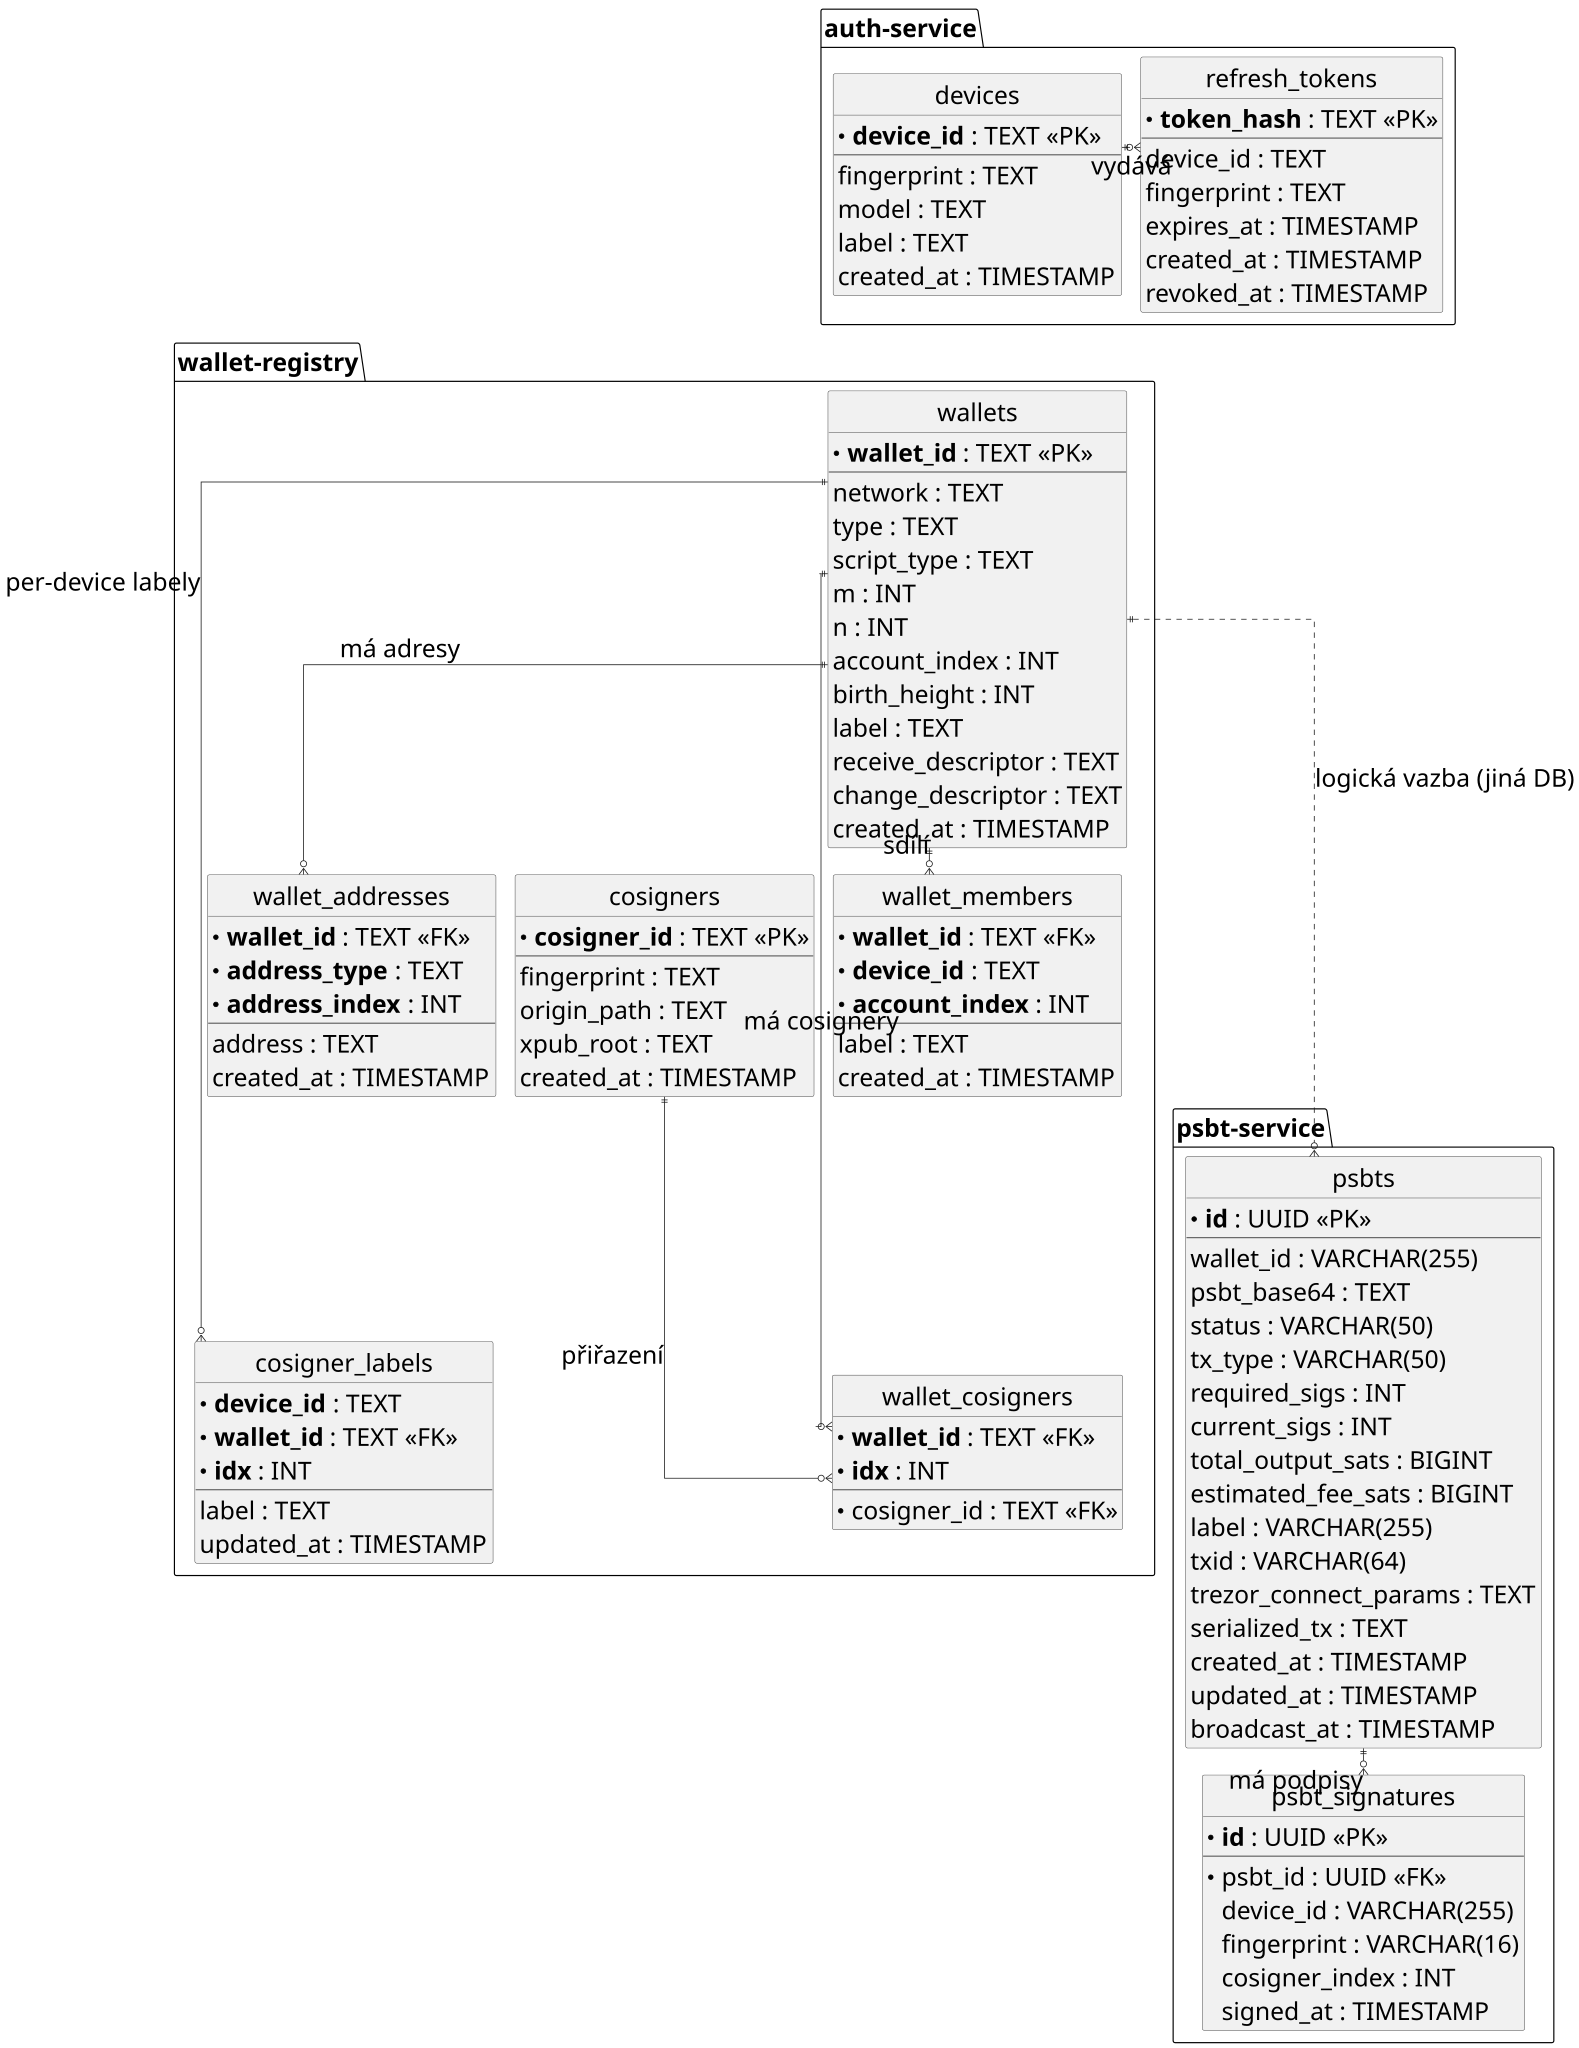
\includegraphics[width=\textwidth]{img/er-diagram.pdf}
\caption{ER diagram datového modelu. Databáze auth-service obsahuje tabulky
zařízení a~refresh tokenů, wallet-registry spravuje peněženky, cosignery,
adresy a~per-device labely, psbt-service uchovává PSBT transakce a~záznamy
podpisů.}
\label{fig:er-diagram}
\end{figure}

\subsection{Databáze PSBT služby}

Databáze \texttt{psbt-service} uchovává transakce v~různých fázích
jejich životního cyklu:

\begin{description}
\item[\texttt{psbts}] -- Hlavní tabulka PSBT transakcí. Obsahuje
  \texttt{id} (UUID, primární klíč),
  \texttt{wallet\_\allowbreak id} (odkaz na~peněženku),
  \texttt{psbt\_\allowbreak base64} (serializovaná PSBT ve~formátu
  Base64), \texttt{status} (pending~/~signed~/~broadcast),
  \texttt{required\_\allowbreak sigs} (požadovaný počet podpisů,
  tj.~$M$), \texttt{current\_\allowbreak sigs} (aktuální počet
  sebraných podpisů),
  \texttt{trezor\_\allowbreak connect\_\allowbreak params} (JSON
  s~parametry pro Trezor Connect, serializovaný do~sloupce typu TEXT)
  a~\texttt{serialized\_\allowbreak tx} (kompletní serializovaná
  transakce po~podpisu, pokud je dostupná).

\item[\texttt{psbt\_\allowbreak signatures}] {\sloppy -- Sleduje, kteří
  cosigneři již PSBT podepsali. Obsahuje
  \texttt{psbt\_\allowbreak id} (cizí klíč na \texttt{psbts.id}),
  \texttt{device\_\allowbreak id} (zařízení, které podepsalo),
  \texttt{fingerprint} (otisk kořenového klíče)
  a~\texttt{cosigner\_\allowbreak index} (index cosignera v~rámci
  peněženky). Tato tabulka zabraňuje duplicitnímu podpisu stejným
  cosignerem.\par}
\end{description}

Parametry pro Trezor Connect ukládáme jako serializovaný JSON
v~textovém sloupci. Jejich struktura závisí na~konkrétní transakci --
počet vstupů a~výstupů se liší, každý vstup má jinou derivační cestu
a~částku~--, ale přes SQL je nikdy nedotazujeme; celý dokument čte
pouze klient, a~to vždy vcelku. Strukturované dotazy a~indexace
(PostgreSQL typ \texttt{JSONB}) by zde proto nepřinesly žádnou výhodu,
a~relační reprezentace by zase vyžadovala zbytečně složité schéma
s~více vazebnými tabulkami. Prostý TEXT je v~tomto případě nejvhodnější
kompromis.

S~tabulkou \texttt{psbts} souvisí ještě jedna nezřejmá implementační
otázka. Při sestavování PSBT si \texttt{psbt-service} eviduje, která UTXO
peněženky jsou aktuálně rezervovaná v~rozpracovaných transakcích, a~při
volbě vstupů pro novou PSBT je vylučuje z~výběru. Bez této rezervace by
mohly vzniknout dvě konkurenční PSBT utrácející tytéž UTXO, z~nichž by
síť přijala jen jednu a~druhá by uvízla v~UI jako zdánlivě platná, ale
trvale nebroadcastovatelná transakce. Rezervace má ale nepříjemný
vedlejší efekt: pokud cosigner u~multisig peněženky nikdy nedokončí
podpis, opuštěný draft drží své vstupy zablokované navždy. Pro řešení
běží v~rámci \texttt{psbt-service} periodická úklidová úloha
(coroutine), která jednou za hodinu odstraní záznamy ve~stavech
\texttt{pending} a~\texttt{signed} starší než sedm dní; broadcastované
transakce zůstávají v~tabulce zachovány jako auditní stopa. Hodnoty
TTL i~intervalu jsou konfigurovatelné přes proměnné prostředí
(\texttt{PSBT\_TTL\_DAYS}, \texttt{PSBT\_CLEANUP\_INTERVAL\_MINUTES}),
celý mechanismus lze pro účely testování vypnout proměnnou
\texttt{PSBT\_CLEANUP\_ENABLED=false}. Uživatel může rozpracovaný draft
také kdykoliv ručně zrušit z~detailu PSBT v~mobilní aplikaci, což má
stejný efekt jako úklidová úloha (smazání řádku, uvolnění
rezervace).

%% -----------------------------------------------------------------------
\section{Návrh PSBT workflow}
\label{sec:psbt-workflow}

Formát PSBT a~zdůvodnění jeho volby pro koordinaci podepisování jsme
popsali v~sekcích~\ref{sec:psbt} a~\ref{sec:analyza-psbt}. Tato sekce
popisuje konkrétní návrh workflow -- jakým způsobem PSBT prochází
systémem od vytvoření po broadcast, jaké stavy nabývá a~jak se liší
singlesig a~multisig flow.

\subsection{Singlesig workflow}

V~případě singlesig peněženky (typ P2WPKH, BIP-84~\cite{BIP84}) probíhá
workflow transakcí ve třech krocích:

\begin{enumerate}
\item \textbf{Vytvoření PSBT} -- Uživatel zadá cílovou adresu, částku
  a~úroveň poplatku. \texttt{psbt-service} vybere UTXO (automaticky nebo
  manuálně dle volby uživatele), sestaví transakci, vypočítá poplatek
  a~vytvoří PSBT včetně parametrů pro Trezor Connect.
\item \textbf{Podpis na Trezoru} -- Mobilní aplikace otevře Trezor Suite
  Mobile s~parametry transakce. Uživatel potvrdí podpis na hardwarové
  peněžence. Trezor vrátí kompletní serializovanou transakci.
\item \textbf{Broadcast} -- Aplikace odešle serializovanou transakci
  na backend, který ji přes \texttt{blockchain-service} propaguje
  do Bitcoinové sítě.
\end{enumerate}

\subsection{Multisig workflow}

Multisig peněženka (typ P2WSH, BIP-48~\cite{BIP48}) ve schématu $M$-of-$N$
vyžaduje podpisy od $M$ z~$N$ cosignerů. Workflow se liší od singlesig
v~tom, že po podpisu prvním cosignerem transakce ještě není kompletní:

\begin{enumerate}
\item \textbf{Vytvoření PSBT} -- Stejné jako u~singlesig. PSBT je uloženo
  se statusem \texttt{pending} a~s~\texttt{current\_sigs = 0}.
\item \textbf{Podpis cosignerem $i$} -- Cosigner otevře detail PSBT v~aplikaci,
  přepne na svůj účet (odpovídající jeho derivační cestě) a~podepíše na
  svém Trezoru. Trezor Connect vrací jak pole podpisů, tak
  \texttt{serializedTx}. Backend z~odpovědi extrahuje pole podpisů,
  uloží je a~inkrementuje \texttt{current\_sigs}.
\item \textbf{Opakování} -- Kroky se opakují pro další cosignery, dokud
  není dosažen práh \texttt{current\_sigs == required\_sigs} ($M$).
\item \textbf{Broadcast} -- Po dosažení prahu je PSBT připraveno k~odeslání.
  Uživatel z~detailu PSBT zvolí broadcast a~backend transakci finalizuje
  a~propaguje do Bitcoin sítě.
\end{enumerate}

Celý multisig podepisovací flow zachycují sekvenční diagramy na
obrázcích~\ref{fig:multisig-signing-1} a~\ref{fig:multisig-signing-2}.

\begin{figure}[htbp]
\centering
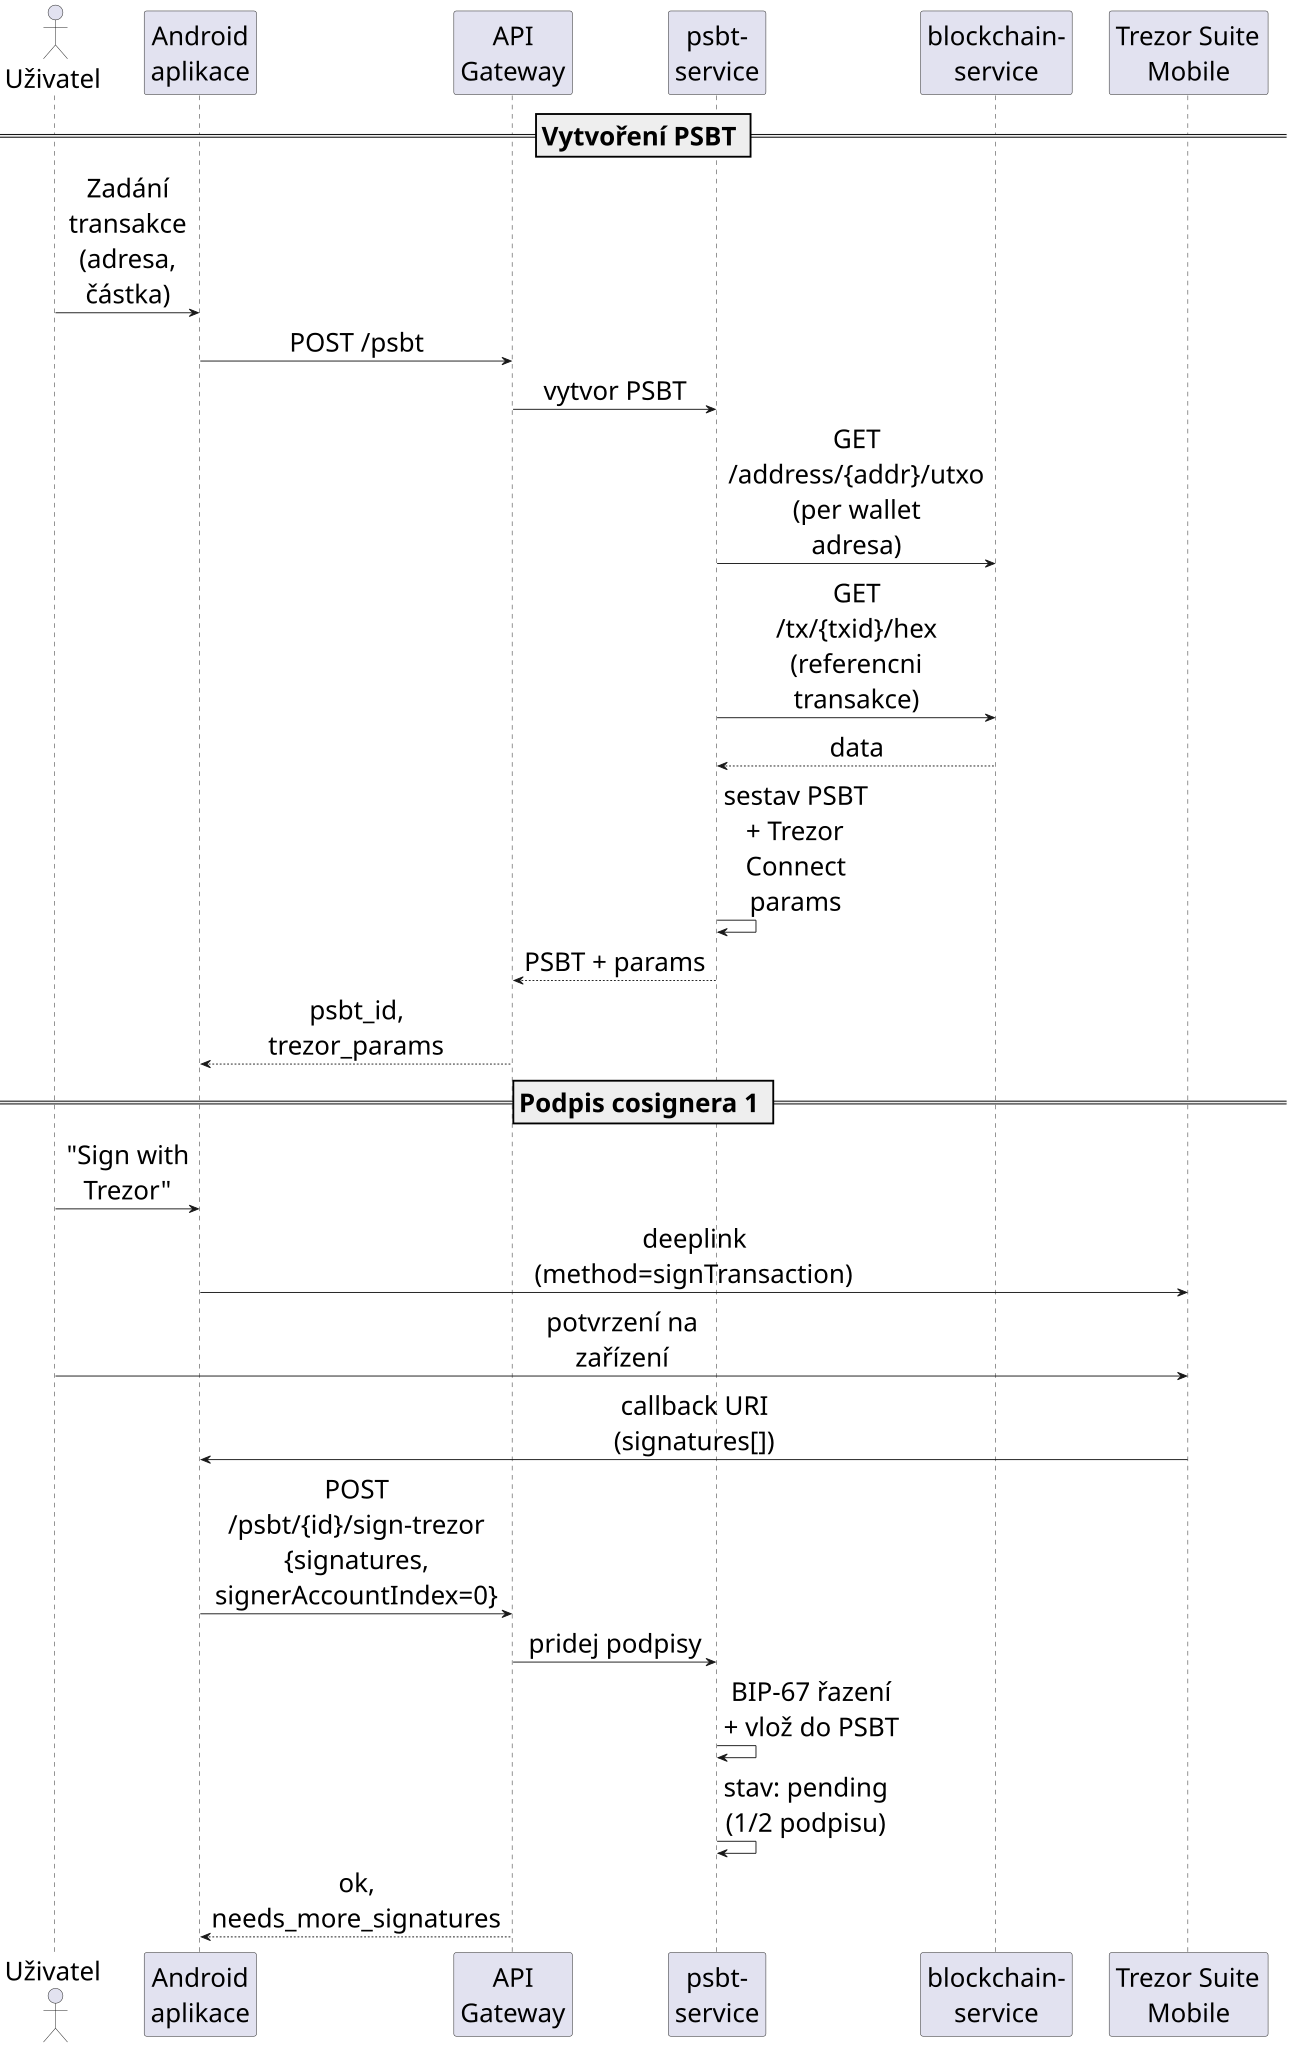
\includegraphics[width=\textwidth,height=0.85\textheight,keepaspectratio]{img/multisig-signing-1.pdf}
\caption{Sekvenční diagram 2-of-3 multisig podepisování -- první část:
vytvoření PSBT a~podpis prvním cosignerem. Backend sestaví PSBT,
mobilní aplikace deleguje podpis na Trezor Suite Mobile a~přidá první podpis.}
\label{fig:multisig-signing-1}
\end{figure}

\begin{figure}[htbp]
\centering
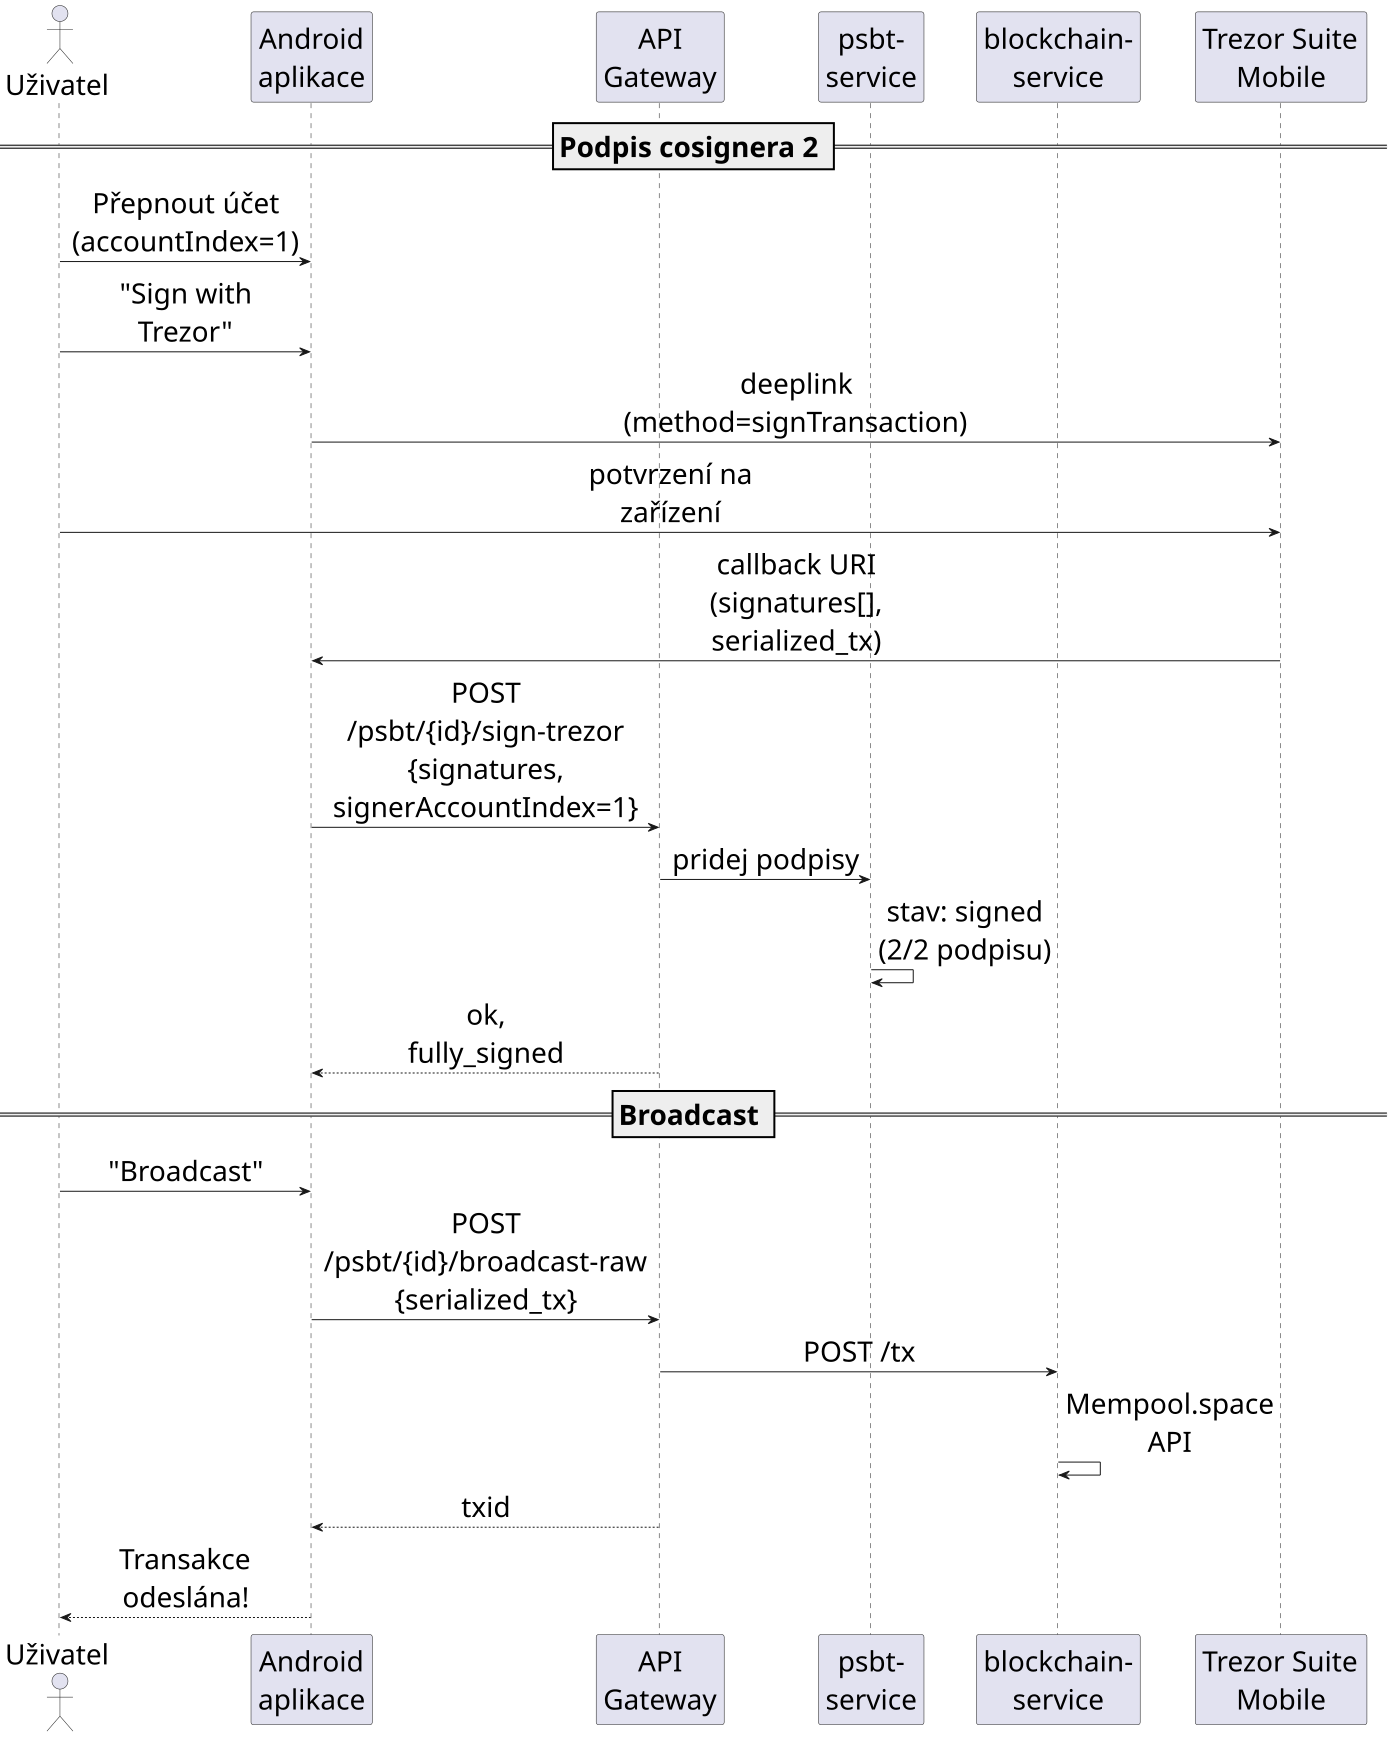
\includegraphics[width=\textwidth,height=0.85\textheight,keepaspectratio]{img/multisig-signing-2.pdf}
\caption{Sekvenční diagram 2-of-3 multisig podepisování -- druhá část:
podpis druhým cosignerem a~broadcast finální transakce. Po dosažení
prahu podpisů uživatel zvolí broadcast a~backend transakci finalizuje
a~odešle do Bitcoinové sítě.}
\label{fig:multisig-signing-2}
\end{figure}

Alternativní přístup k~multisig podepisování by bylo předávání PSBT
souboru mezi cosignery (například prostřednictvím QR kódů nebo SD karet),
jak to implementuje například Sparrow Wallet~\cite{SparrowWallet}. Tento
\emph{offline} přístup je bezpečnější z~hlediska soukromí, protože nevyžaduje
centrální server. V~kontextu mobilní aplikace je však nepraktický --
uživatel by musel manuálně exportovat a~importovat PSBT soubory. Zvolený
serverový přístup umožňuje, aby cosigneři jednoduše otevřeli seznam
čekajících transakcí v~aplikaci a~podepsali jedním kliknutím.

\subsection{Výběr UTXO a coin control}
\label{subsec:coin-control}

Při tvorbě transakce je nutné vybrat, které nepoužité výstupy (UTXO) budou
použity jako vstupy. Aplikace nabízí dva režimy:

\begin{description}
\item[Automatický výběr] -- Systém vybírá UTXO strategií \emph{largest-first}:
  řadí dostupné UTXO sestupně podle hodnoty a~přidává je, dokud součet
  nepřekročí požadovanou částku včetně poplatku. Tato strategie minimalizuje
  počet vstupů (a~tedy velikost a~poplatek transakce), ale může vést
  k~suboptimálnímu výběru z~hlediska soukromí, protože spojuje velké UTXO.

\item[Manuální výběr (coin control)] -- Uživatel sám vybírá konkrétní UTXO,
  které chce utratit. Tato pokročilá funkce umožňuje uživateli řídit, které
  adresy a~částky vstupují do transakce, což je důležité pro zachování
  soukromí (zamezení spojování UTXO z~různých zdrojů) a~pro řízení
  konsolidace prostředků.
\end{description}

Zvažovali jsme i~pokročilejší algoritmy výběru UTXO, jako je
\emph{Branch and Bound} (používaný v~Bitcoin Core), který hledá přesný součet
bez nutnosti change výstupu. Pro první verzi aplikace jsme zvolili jednodušší
strategii \emph{largest-first}, která je dostatečná pro většinu případů
použití a~je snadno předvídatelná pro uživatele.

\subsection{Výpočet poplatku}

Poplatek za transakci se v~Bitcoin síti odvíjí od velikosti transakce
ve virtuálních bytech (vBytes), nikoliv od převáděné částky. Virtuální
velikost se dle BIP-141~\cite{BIP141} vypočítá jako:

\[
\mathit{vSize} = \left\lceil \frac{\mathit{weight}}{4} \right\rceil, \quad
\mathit{weight} = \mathit{base\_size} \times 3 + \mathit{total\_size}
\]

\noindent kde \emph{base\_size} je velikost transakce bez witness dat
a~\emph{total\_size} zahrnuje i~witness. Díky tomuto vzorci mají witness
data (podpisy) čtyřikrát nižší váhu než ostatní části transakce, což je
motivace pro přechod na SegWit adresy.

Odhad velikosti závisí na typu peněženky:

\begin{itemize}
\item \textbf{P2WPKH (singlesig)} -- každý vstup přidá přibližně 68~vB
  (41~B non-witness: outpoint 36~B, sequence 4~B, délka skriptu 1~B;
  plus witness: 1~B počet položek, ${\approx}72$~B DER podpis,
  33~B komprimovaný veřejný klíč). Každý výstup přidá přibližně 31~vB
  a~fixní režie transakce (verze, počty, locktime) činí přibližně 10~vB.

\item \textbf{P2WSH (multisig)} -- vstup je výrazně větší, protože
  witness musí obsahovat $M$~podpisů a~kompletní redeem skript s~$N$
  veřejnými klíči. Non-witness část zůstává 41~B, ale witness data
  rostou: úvodní \texttt{OP\_0} (${\approx}6$~B s~délkami), $M$~podpisů
  (každý maximálně 73~B: DER-kódovaný ECDSA podpis plus push opcode)
  a~redeem skript ($N \times 34$~B pro komprimované veřejné klíče plus
  opcodes \texttt{OP\_M}, \texttt{OP\_N}, \texttt{OP\_CHECKMULTISIG}).
  Velikost vstupu odhadujeme dle výpočtu popsaného
  v~sekci~\ref{sec:p2wsh-multisig} jako $41 + (6 + 73M + 34N)/4$~vB.
  Například pro schéma 2-of-3: $41 + (6 + 146 + 102)/4 \approx 105$~vB
  na vstup.
\end{itemize}

Celková odhadovaná velikost transakce je tedy:

\[
\mathit{vSize}_{\text{odhad}} = \text{režie} + n_{\text{vstupů}} \times \mathit{vSize}_{\text{vstup}} + n_{\text{výstupů}} \times 31 \;\text{vB}
\]

\noindent Tato hodnota se vynásobí aktuální sazbou poplatku (v~sat/vB),
kterou uživatel volí z~nabídky tří úrovní: nízký poplatek (odhad pro
potvrzení do jedné hodiny), střední (do třiceti minut) a~vysoký (nejbližší
blok). Sazby pro jednotlivé úrovně aplikace získává z~blockchainového API,
které je odvozuje z~aktuálního stavu mempoolu -- fronty nepotvrzených
transakcí čekajících na zařazení do bloku~\cite{MempoolAPI}. V~režimu
manuálního výběru UTXO může uživatel alternativně zadat libovolnou sazbu
v~sat/vB ručně.

\subsection{Zpracování change výstupu}

Pokud součet vybraných UTXO překračuje požadovanou částku včetně poplatku,
vytvoří se change výstup vracející přebytek zpět do peněženky na novou
change adresu. Existuje však speciální případ: pokud by hodnota change
výstupu byla menší než tzv.~\emph{dust threshold}, change výstup se
nevytváří a~celý přebytek se přidá k~poplatku. Vytvořením výstupu pod
prahem by transakce nebyla standardní a~uzly v~síti by ji odmítly propagovat.
Dust threshold závisí na typu výstupu: pro P2PKH je 546~satoshi,
pro P2WPKH 294~satoshi a~pro P2WSH 330~satoshi. V~implementaci
používáme konzervativní hodnotu 546~satoshi bez ohledu na typ výstupu,
čímž garantujeme, že žádný výstup nebude uzly odmítnut.

%% -----------------------------------------------------------------------
\section{Návrh uživatelského rozhraní}
\label{sec:ui-navrh}

\subsection{Architektonický vzor MVVM}

Pro organizaci kódu mobilní aplikace jsme zvolili architektonický vzor
MVVM (\emph{Model--View--ViewModel}), který je doporučeným přístupem
pro Android aplikace s~Jetpack Compose. Jednotlivé vrstvy mají tyto role:

\begin{description}
\item[Model] -- Datové třídy reprezentující doménové entity (peněženka,
  transakce, UTXO, PSBT) a~repozitáře zajišťující komunikaci s~backendem
  prostřednictvím REST API.
\item[ViewModel] -- Obsahuje prezentační logiku a~udržuje stav obrazovky.
  Stav je reprezentován Kotlinovým \texttt{StateFlow}, na jehož změny
  se Compose UI automaticky přehlásí a~překreslí dotčené komponenty.
  ViewModel přežívá změnu konfigurace (otočení obrazovky) díky integraci
  s~Android lifecycle.
\item[View (Composable)] -- Deklarativní Compose funkce, které vykreslují
  UI na základě stavu z~ViewModelu. Neobsahují žádnou business logiku
  a~jsou snadno testovatelné a~znovupoužitelné.
\end{description}

Alternativou by byl vzor MVI (\emph{Model--View--Intent}), který je
přísnější v~tom, že veškeré uživatelské akce modeluje jako unidirektionální
proud intentů. MVI nabízí lepší predikovatelnost stavu, ale za cenu vyššího
množství boilerplate kódu. Pro rozsah aplikace je MVVM dostatečný
a~lépe odpovídá konvencím Android ekosystému.

\subsection{Navigační struktura}

Navigace v~aplikaci sleduje lineární tok s~možností návratu:

\begin{enumerate}
\item \textbf{Připojení Trezoru} -- Úvodní obrazovka, kde uživatel připojí
  Trezor přes deeplink do Trezor Suite Mobile. Aplikace vyžádá export xpub
  pro deset účtů (BIP-84).
\item \textbf{Skenování účtů} -- Backend provede account discovery, ověří
  aktivitu na blockchainu a~vytvoří singlesig peněženky pro účty
  s~transakční historií.
\item \textbf{Výběr singlesig účtu} -- Uživatel vybere jeden ze singlesig
  účtů odvozených z~Trezoru. Multisig peněženky se zde nezobrazují --
  ty jsou přidružené k~singlesig účtům a~přístupné přes navigační menu.
\item \textbf{Dashboard} -- Hlavní obrazovka zobrazující zůstatek vybraného
  singlesig účtu (v~BTC i~ve zvolené fiat měně), seznam transakcí
  a~tlačítka pro odeslání a~příjem. Postranní navigační menu
  (\emph{drawer}) umožňuje přechod na seznam multisig peněženek
  a~nastavení.
\item \textbf{Multisig peněženky} -- Seznam importovaných multisig peněženek
  přidružených k~aktuálnímu zařízení. Po výběru peněženky se zobrazí
  její vlastní dashboard se zůstatkem, transakcemi a~přístupem
  k~seznamu PSBT transakcí.
\end{enumerate}

Přehled navigační struktury a~přechodů mezi obrazovkami zachycuje
obrázek~\ref{fig:navigation}.

\begin{figure}[htbp]
\centering
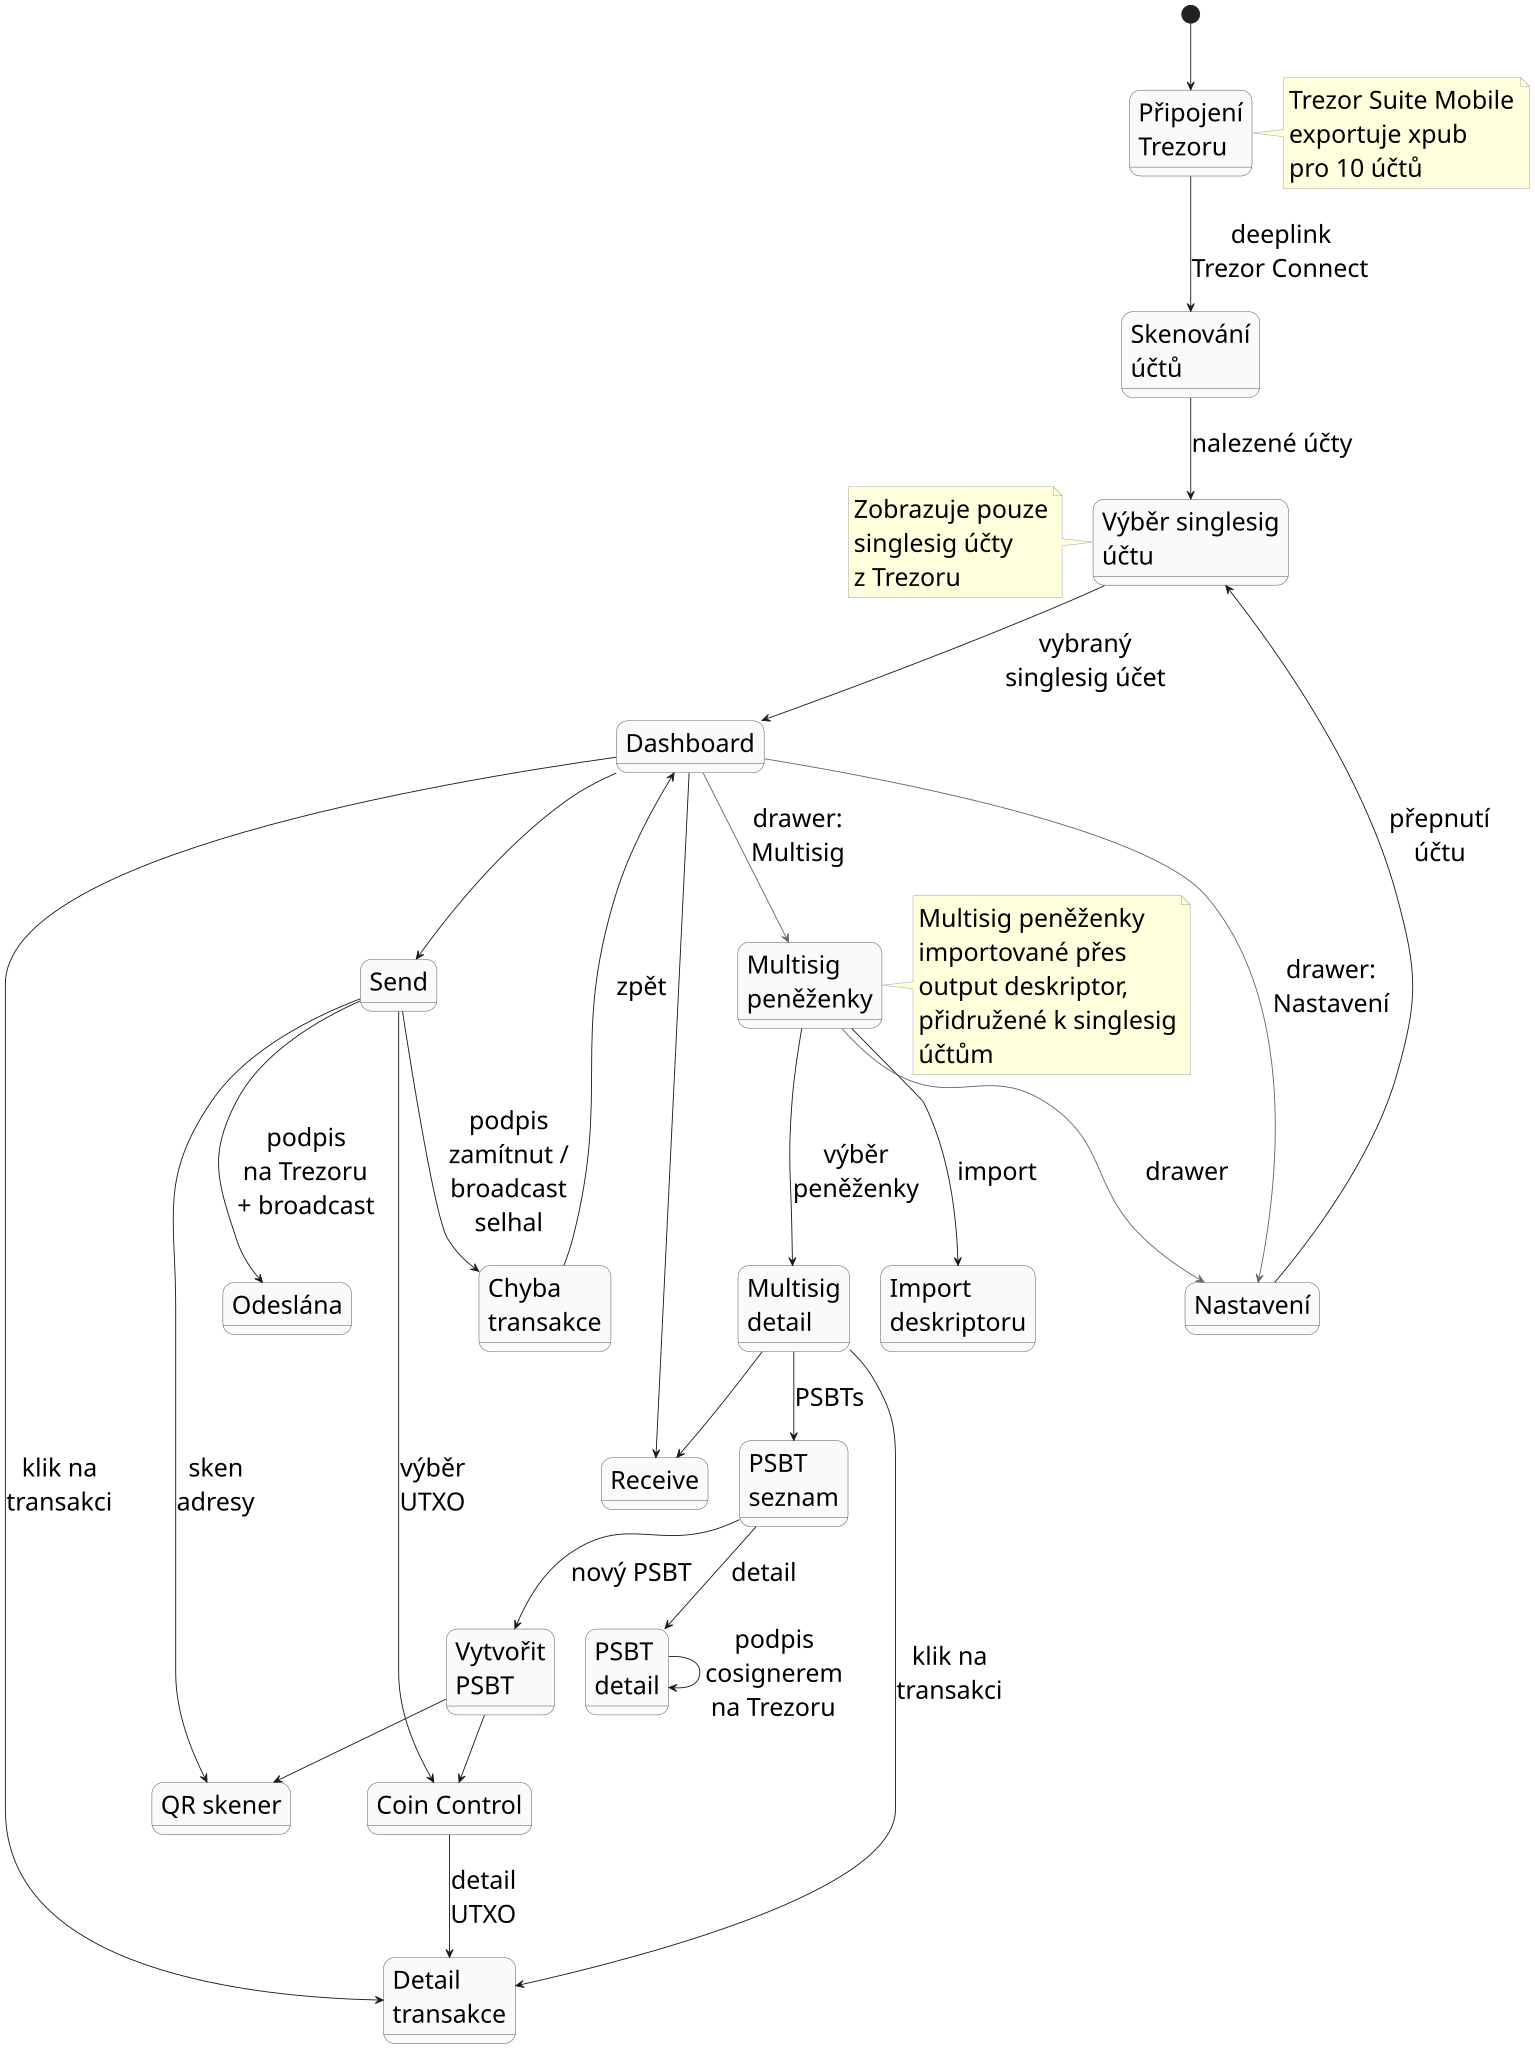
\includegraphics[width=\textwidth]{img/navigation.pdf}
\caption{Navigační diagram aplikace. Po připojení Trezoru uživatel vybere
singlesig účet a~vstoupí na dashboard. Multisig peněženky jsou přístupné
přes postranní menu a~mají vlastní detail se seznamem PSBT. Šedé šipky
značí navigaci přes drawer menu.}
\label{fig:navigation}
\end{figure}

\subsection{Klíčové obrazovky}

\begin{description}
\item[Dashboard] -- Zobrazuje zůstatek peněženky, konverzi do fiat měny
  a~chronologický seznam transakcí s~potvrzeními. Pro multisig peněženku
  navíc zobrazuje počet čekajících PSBT vyžadujících podpis.

\item[Detail transakce] -- Rozklikem libovolné položky ze seznamu
  transakcí na dashboardu. Zobrazuje \texttt{txid}, stav potvrzení, výšku
  bloku, časové razítko, poplatek včetně sazby v~sat/vB a~seznam vstupů
  a~výstupů s~částkami. Adresy patřící aktuální peněžence jsou označeny
  štítkem \emph{YOURS}. Kliknutím na vstup lze otevřít předchozí transakci,
  která daný UTXO vytvořila, a~procházet tak historii až do hloubky pěti
  úrovní; na každé úrovni je štítkem \emph{FROM HERE} označen výstup, který
  navazuje na proklikaný vstup z~úrovně předchozí. Hloubka je omezená,
  aby nedošlo k~nadměrnému zatížení blockchainového API. Tato funkce slouží
  uživateli k~forenznímu ověření původu prostředků bez nutnosti přepínat
  do externího prohlížeče blockchainu.

\item[Send (odeslání)] -- Formulář pro zadání cílové adresy (manuálně
  nebo skenováním QR kódu), částky, volby úrovně poplatku a~volitelně
  manuálního výběru UTXO (coin control). Po vyplnění formuláře se zobrazí
  souhrn transakce a~uživatel potvrdí odeslání, čímž se zahájí podepisování
  na Trezoru.

\item[Receive (příjem)] -- Zobrazuje aktuální přijímací adresu peněženky
  ve formě QR kódu a~textového řetězce s~možností kopírování do schránky.
  Tlačítko \emph{Zobrazit na Trezoru} umožňuje ověřit adresu na displeji
  hardwarové peněženky (viz popis v~sekci~\ref{subsec:trezor-connect}).

\item[PSBT seznam] -- Přístupný pouze pro multisig peněženky. Zobrazuje
  seznam vytvořených PSBT transakcí s~jejich stavem (čekající na podpisy /
  podepsaná / broadcastovaná). U~čekajících transakcí zobrazuje, kolik
  podpisů zbývá do prahu.

\item[PSBT detail] -- Detail konkrétní PSBT transakce se souhrnem částky,
  poplatku a~celkové hodnoty. Zobrazuje stav podpisů jednotlivých cosignerů --
  u~každého cosignera je vidět, zda podepsal, a~v~dialogu signerů si uživatel
  může cosignerům přiřadit vlastní pojmenování (například ,,Alicin klíč``).
  Tento název je privátní pro dané zařízení -- uloží se vázaný na
  \texttt{device\_id} přihlášeného Trezoru a~ostatním cosignerům se nezobrazí.
  Důvodem je ochrana soukromí: osobní poznámky o~spolupodepisovatelích by
  neměly prosakovat mezi členy sdílené peněženky. Pokud transakce čeká
  na podpis aktuálního cosignera, zobrazí se tlačítko pro podepsání.

\item[Nastavení] -- Umožňuje přepnutí aktivního účtu (pro multisig testování
  s~více cosignery na jednom zařízení), výběr fiat měny pro zobrazení
  ekvivalentu zůstatku (CZK, USD nebo EUR), import output deskriptoru pro
  vytvoření multisig peněženky a~zobrazení informací o~aplikaci
  a~připojeném zařízení.
\end{description}

Při návrhu obrazovek jsme kladli důraz na přehlednost a~bezpečnost.
Před odesláním každé transakce se zobrazí kompletní souhrn (cílová adresa,
částka, poplatek), aby uživatel měl poslední možnost ověřit správnost
údajů před potvrzením na hardwarové peněžence. Detaily transakce
uživatel vždy ověřuje ještě na displeji samotného Trezoru, což poskytuje
nezávislou kontrolu proti případné kompromitaci mobilní aplikace.

%% -----------------------------------------------------------------------
\section{Implementační detaily}
\label{sec:impl-detaily}

V~této sekci popisujeme vybrané implementační problémy a~technické výzvy,
které přesahují rámec architektonického návrhu a~které považujeme
za zajímavé z~hlediska pochopení fungování systému.

\subsection{Sestavení binární struktury PSBT}

Třída \texttt{PsbtBuilder} v~modulu \texttt{psbt-service} sestavuje kompletní
binární strukturu PSBT dle BIP-174~\cite{BIP174}. Formát začíná magic sekvencí
\texttt{0x70736274ff} (ASCII \uv{psbt} + separátor), následovanou globální sekcí
s~nepodepsanou transakcí, per-input sekcemi s~metadaty pro podepisování
a~per-output sekcemi s~derivačními cestami. Každá sekce je ukončena nulovým bajtem.

Pro každý vstup zapisujeme čtyři typy záznamů:
\begin{itemize}
\item \texttt{PSBT\_IN\_NON\_WITNESS\_UTXO} -- celá předchozí transakce v~raw
  formátu. Firmware Trezor od verze~2.3.1 vyžaduje tento záznam i~pro nativní
  SegWit vstupy~\cite{TrezorFirmwareDocs}, aby mohl ověřit částky vstupů
  a~zobrazit správný poplatek.
\item \texttt{PSBT\_IN\_WITNESS\_UTXO} -- částka a~scriptPubKey utrácené UTXO.
\item \texttt{PSBT\_IN\_WITNESS\_SCRIPT} -- witness skript multisig transakce
  (pouze pro P2WSH) se~všemi veřejnými klíči v~BIP-67 pořadí.
\item \texttt{PSBT\_IN\_BIP32\_DERIVATION} -- derivační cesta pro každého
  cosignera, aby Trezor identifikoval svůj klíč.
\end{itemize}

\noindent Pro change výstup přidáváme \texttt{PSBT\_OUT\_BIP32\_DERIVATION},
aby peněženka rozpoznala, že change směřuje zpět na~vlastní adresu.

\subsection{Převod PSBT na parametry Trezor Connect}

Trezor Connect nepřijímá PSBT přímo -- vyžaduje strukturovaný JSON
s~explicitními derivačními cestami, multisig metadaty a~referenčními
transakcemi~\cite{TrezorConnect,TrezorFirmwareDocs}. Třída
\texttt{TrezorParamsBuilder} provádí tento převod.

Pro singlesig transakce je převod přímočarý: každý vstup obsahuje
derivační cestu jako pole uint32 hodnot (hardened indexy s~bitem
\texttt{0x80000000}), hash a~index předchozí transakce, částku a~typ
skriptu. Change výstup místo cílové adresy obsahuje derivační cestu,
aby Trezor poznal interní výstup.

Pro multisig transakce vyžaduje každý vstup navíc objekt \texttt{multisig}
obsahující pole \texttt{pubkeys} (strukturovaný \texttt{HDNodeType} místo
xpub řetězce), práh~$M$ a~pole \texttt{signatures} (prázdné řetězce pro
dosud nepodepsané pozice). Pořadí klíčů musí přesně odpovídat BIP-67
řazení pro daný vstup -- Trezor firmware řazení neprovádí interně.

Trezor Connect dále vyžaduje referenční transakce v~parsované podobě
(ne raw hex), proto backend pro každý vstup stáhne předchozí
transakci z~\texttt{blockchain-\allowbreak service} a~převede ji
na~strukturovaný formát s~poli \texttt{version}, \texttt{inputs},
\texttt{bin\_\allowbreak outputs} a~\texttt{lock\_\allowbreak time}.

\subsection{BIP-67 řazení podpisů ve witness}

Jednou z~nejobtížnějších chyb, na které jsme při vývoji narazili, bylo
správné řazení podpisů ve~witness stacku multisig transakce. Podpisy
musí být umístěny ve~stejném pořadí jako odpovídající veřejné klíče
ve~witness skriptu. Protože \texttt{sortedmulti} deskriptory řadí klíče
lexikograficky dle BIP-67~\cite{BIP67}, nemusí se~toto pořadí shodovat
s~pořadím cosignerů podle jejich indexu.

Původní implementace umísťovala podpis na~pozici odpovídající
\texttt{cosigner\-Index}. To fungovalo, pouze dokud se~lexikografické
pořadí náhodou shodovalo s~pořadím cosignerů. Chyba se~projevila
až při testování s~cosignerem, jehož veřejný klíč byl po~BIP-67 řazení
na~jiné pozici. Po~opravě systém pro každý vstup zvlášť odvodí child
pubkeys všech cosignerů, seřadí je lexikograficky a~podpis umístí
na~odpovídající pozici.

\subsection{Předcházení reuse change adres}

Další chyba, která se~projevila až při testování s~reálnými prostředky,
se~týkala výběru change adresy při sestavování PSBT. Původní implementace
volala \texttt{wallet-registry} s~pevně zadaným indexem~0, což znamenalo,
že \emph{každá} odchozí transakce posílala svůj change výstup na tutéž
adresu. Nebylo to okamžitě viditelné, protože adresa se~v~UI nikdy
nezobrazuje -- uživatel ji vidí jen v~prohlížeči blockchainu nebo při
detailním procházení historie. Při opakovaných odchozích transakcích
tak vznikal řetězec, kde se~stejná adresa opakovaně objevovala jako
vstup i~jako change výstup, což je anti-pattern z~hlediska soukromí:
pozorovatel blockchainu může všechny takové transakce triviálně spojit
do jediného klastru a~odhadnout celkový zůstatek i~aktivitu peněženky.

Oprava vyžadovala zavést novou komponentu pro výběr adres s~kontrolou
on-chain aktivity. Službu \texttt{explorer-service} jsme rozšířili
o~endpoint vracející první change adresu bez transakční historie, což
je analogie již existující logiky pro přijímací adresy. Pokud jsou
všechny adresy v~rámci počátečního gap limitu~20 již použité, zavolá
se~nově zavedený endpoint \texttt{wallet-registry} pro~odvození dalšího
indexu za gap limit a~jeho zápis do databáze. Služba \texttt{psbt-service}
si tak pro každou novou PSBT vyžádá čerstvou change adresu, a~řetězec
opakovaných výskytů byl definitivně rozbit.

\subsection{Rate limiting blockchainového API}

Služba \texttt{blockchain-service} řeší rate limiting
Mempool.space API, které při překročení souběžných požadavků vrací
HTTP~429. Při stahování dat pro celou peněženku (až 40~adres paralelně)
k~tomu snadno dojde. Implementovali jsme omezení pomocí Kotlin coroutine
\texttt{Semaphore} s~limitem 5~souběžných požadavků a~jedním retry
s~jednosekundovým zpožděním při selhání. Více pokusů záměrně neprovádíme --
pokud je IP adresa v~\uv{penalty box}, opakované pokusy pouze prodlužují
frontu.

\subsection{Agregace dat peněženky}

Služba \texttt{explorer-service} řeší tzv.\ N+1~problém: frontend potřebuje
zobrazit data celé peněženky (zůstatek, transakce, UTXO), ale blockchainové
API pracuje na~úrovni jednotlivých adres. Pro peněženku se 40~adresami
(20~receive + 20~change) by naivní přístup vyžadoval 40~HTTP volání.
Implementovali jsme dvoustupňovou optimalizaci: nejprve jedním lehkým
voláním zjistíme \texttt{tx\_count} pro každou adresu a~přeskočíme neaktivní,
poté pro aktivní adresy stahujeme detailní data paralelně. Tím se počet
volání typicky sníží na~5--10.

\subsection{Signing interface}

Jak jsme analyzovali v~sekci~\ref{sec:analyza-trezor}, architektura aplikace
je navržena s~čistým interním rozhraním pro podepisování. V~aktuální verzi
je implementováno prostřednictvím deeplinků do Trezor Suite Mobile, ale
abstrakce je připravena tak, aby bylo možné v~budoucnu přidat přímou USB
komunikaci s~Trezorem jako alternativní implementaci bez nutnosti změn
ve~zbytku systému. Třída \texttt{TrezorDeeplinkLauncher} na frontendu
zapouzdřuje veškerou logiku komunikace s~Trezor Connect -- volající kód
pracuje pouze s~metodami \texttt{openGetPublicKey} a~\texttt{openSignTransaction}
a~nezná implementační detaily deeplink protokolu.

%\include{kap-implementace}
%%% Kapitola 4: Testování

\chapter{Testování}
\label{chap:testovani}

Cílem testování bylo ověřit, že navržená aplikace splňuje funkční požadavky
formulované v~kapitole~\ref{chap:specifikace} -- zejména že dokáže přihlásit
uživatele přes Trezor, správně sestavit a~odeslat singlesig transakci a~že celý
multisig workflow od importu deskriptoru přes postupné podepisování až po
broadcast funguje proti reálnému Bitcoinovému uzlu. V~této kapitole popisujeme
zvolený přístup k~testování, jeho odůvodnění, použité prostředí, provedené
scénáře a~nakonec chyby, které jsme díky testování odhalili.

%%% -----------------------------------------------------------------------
\section{Zvolený přístup}
\label{sec:test-pristup}

Při návrhu testovací strategie jsme zvažovali tři varianty.

První možností byla \textbf{automatizovaná sada unit testů} pokrývající
jednotlivé komponenty backendu (parsing deskriptorů, derivaci adres,
sestavování PSBT). Tento přístup poskytuje rychlou zpětnou vazbu při
změnách kódu a~je standardem pro produkční software. V~kontextu naší
aplikace by však unit testy izolovaly právě ty části, kde jsme reálně
nehledali chyby -- kryptografická logika je delegována na knihovnu
bitcoinj~\cite{BitcoinJ}, derivace probíhá podle dobře definovaných BIP
standardů a~lze ji ověřit proti existujícím peněženkám. Naopak by neodhalily
problémy v~integraci s~Trezorem, protože ten je v~unit testech nahrazen
mockem, který se na rozdíl od skutečného firmware chová tolerantně.

Druhou možností byly \textbf{end-to-end testy s~emulátorem Trezoru}, který
SatoshiLabs poskytuje pro vývojové účely. Tento přístup by umožnil
automatizovat i~podepisovací krok. Komunikace s~emulátorem však vyžaduje
implementaci části protokolu Trezor Connect, což je přesně to, čemu se
naše architektura záměrně vyhýbá delegováním na Trezor Suite Mobile (viz
sekci~\ref{sec:analyza-trezor}). Pro testovací sadu by tak bylo nutné
vyvinout paralelní komunikační vrstvu, která by se v~samotné aplikaci
vůbec nepoužila. To jsme v~rámci bakalářské práce vyhodnotili jako úsilí
neúměrné přínosu.

Zvolili jsme proto třetí variantu: \textbf{manuální integrační testování
proti Bitcoin testnetu} s~reálnou hardwarovou peněženkou Trezor.
Tento přístup ověřuje právě ty integrační body, kde reálně vznikají chyby --
komunikaci mezi mobilní aplikací, Trezor Suite Mobile a~hardwarovým
zařízením, korektnost sestavených PSBT z~pohledu firmware Trezoru
a~validitu výsledných transakcí z~pohledu Bitcoinové sítě. Cenou je nutnost
manuálně procházet všechny scénáře při každé větší změně, což akceptujeme
vzhledem k~omezenému rozsahu funkcionality. Doplnění automatizované testovací
sady považujeme za vhodný směr dalšího vývoje.

%%% -----------------------------------------------------------------------
\section{Testovací prostředí}
\label{sec:test-prostredi}

Veškeré testování probíhalo proti síti testnet4. Testnetové prostředky
(tBTC) jsme získávali z~veřejně dostupných faucetů -- webových služeb, které
bezplatně distribuují malé množství testnetových mincí vývojářům pro účely
testování.

Backend byl spuštěn lokálně pomocí Docker Compose~\cite{Docker} -- jednou
spuštěný stack obsahoval všech šest mikroslužeb popsaných
v~sekci~\ref{sec:architektura},
API Gateway, tři instance PostgreSQL~\cite{PostgreSQL} a~síťové připojení na
veřejné API Mempool.space~\cite{MempoolAPI} pro testnet4. Mobilní aplikace
běžela na fyzickém Android zařízení se soubežně nainstalovanou aplikací
Trezor Suite Mobile, která zprostředkovává komunikaci s~hardwarovou peněženkou
podle deeplink protokolu popsaného v~sekci~\ref{subsec:trezor-connect}.
K~testování jsme využili jednu hardwarovou peněženku Trezor s~inicializovaným
seedem.

Pro multisig scénáře 2-of-3 vyvstává otázka, jak simulovat tři nezávislé
cosignery, když máme k~dispozici pouze jedno fyzické zařízení. Zvolili jsme
přístup, kdy na témže Trezoru používáme tři různé účty podle BIP-48~\cite{BIP48}
s~derivačními cestami \texttt{m/48'/1'/0'/2'}, \texttt{m/48'/1'/1'/2'}
a~\texttt{m/48'/1'/2'/2'}. Z~pohledu kryptografického protokolu jsou tyto účty
plnohodnotnými nezávislými klíčovými páry -- BIP-32 garantuje, že odvozené
klíče různých větví spolu nesouvisí způsobem, který by šel z~veřejných dat
detekovat. Aplikace přitom mezi účty přepíná na úrovni session a~Trezor pro
každý podpis vyžaduje samostatné fyzické potvrzení, takže z~hlediska workflow
se postup neliší od reálného nasazení s~více zařízeními. Jediné, co tento
přístup neověří, je souběžné podepisování více uživateli v~čase; v~našem
sériovém workflow však k~souběhu beztak nedochází, protože PSBT se mezi
cosignery předává postupně.

Multisig deskriptor jsme vytvářeli v~aplikaci Sparrow Wallet~\cite{SparrowWallet},
do které jsme z~Trezoru exportovali tři xpub klíče, nakonfigurovali peněženku
2-of-3 a~deskriptor ve formátu \texttt{wsh(sortedmulti(2,...))} jsme zkopírovali
do importního dialogu naší aplikace. Sparrow zároveň sloužil jako referenční
peněženka -- adresy odvozené naší aplikací jsme porovnávali s~adresami, které
pro stejný deskriptor zobrazil Sparrow, a~v~prohlížeči blockchainu Mempool.space
jsme nezávisle ověřovali stav transakcí.

%%% -----------------------------------------------------------------------
\section{Provedené scénáře}
\label{sec:test-scenare}

Testovací scénáře jsme odvodili z~případů užití definovaných
v~sekci~\ref{sec:use-cases}. Pro každý use case existuje odpovídající
manuální scénář; níže je popisujeme stručně, pouze z~hlediska toho, co
ověřují a~co je u~nich kritické.

\textbf{Singlesig workflow.} Začínáme přihlášením uživatele přes Trezor
(UC1). Aplikace vyžádá z~hardwarové peněženky deset xpub klíčů pro účty
\texttt{m/84'/1'/0'} až \texttt{m/84'/1'/9'}, backend pro každý xpub provede
account discovery dle BIP-44~\cite{BIP44} a~vrátí seznam aktivních
singlesig peněženek. Tento scénář ověřuje, že deeplink komunikace s~Trezor
Suite Mobile funguje a~že JWT token vydaný službou \texttt{auth-service}
umožní následný přístup k~ostatním službám.

Dalším scénářem je odeslání singlesig transakce typu P2WPKH (UC2). Zadáme
testnetovou adresu, částku a~úroveň poplatku, aplikace nás přes deeplink
přesměruje do Trezor Suite Mobile, kde transakci podepíšeme na zařízení.
Po návratu callback URL aplikace odešle serializovanou transakci na
backend, který provede broadcast přes \texttt{blockchain-service}. Úspěšnost
ověřujeme jednak hlášením z~aplikace (zobrazení txid), jednak vyhledáním
této transakce v~Mempool.space. Variantou tohoto scénáře je test funkce
coin control (UC5), kdy před potvrzením ručně vybereme konkrétní UTXO --
ověřujeme, že výsledná transakce na blockchainu obsahuje právě jeden vstup
odpovídající zvolenému UTXO a~že odhad poplatku se přepočítal podle nového
počtu vstupů.

Příjem prostředků (UC z~user story~US4) testujeme tak, že v~aplikaci
zobrazíme přijímací adresu, z~externího faucetu na ni odešleme malou částku
tBTC a~ověřujeme, že po potvrzení transakce se zůstatek v~aplikaci aktualizuje
a~v~historii se objeví příchozí transakce se správnou klasifikací směru
(\textit{received}, nikoli \textit{sent}).

\textbf{Multisig workflow.} Po importu deskriptoru (UC3) ověřujeme, že
aplikace zobrazí novou peněženku s~informací ,,2-of-3``, že odvozené adresy
začínají prefixem \texttt{tb1q} a~jsou shodné s~adresami, které pro tentýž
deskriptor zobrazí Sparrow Wallet, a~že zobrazený zůstatek odpovídá
prostředkům, které jsme na multisig adresy předem odeslali z~faucetu.

Hlavním scénářem multisig části je vytvoření, podepsání a~broadcast 2-of-3
transakce (UC4 + UC6). Postup probíhá ve čtyřech krocích: nejprve jako
cosigner~1 (\texttt{m/48'/1'/0'/2'}) zadáme cílovou adresu a~částku, backend
sestaví PSBT pro multisig vstupy a~aplikace nás přes deeplink odešle k~podpisu
na Trezor. Trezor v~multisig režimu vrací pouze pole podpisů, nikoli celou
serializovanou transakci -- tyto podpisy backend přidá do PSBT na pozici
odpovídající aktuálnímu cosignerovi. Stav PSBT přejde z~\texttt{pending}
(0~podpisů) na 1~ze~2 a~aplikace zobrazí informaci, že transakce čeká na
dalšího cosignera. Ve druhém kroku v~nastavení přepneme aktivní účet na
cosignera~2 (\texttt{m/48'/1'/1'/2'}), v~seznamu rozpracovaných PSBT vybereme
připravovanou transakci a~znovu projdeme deeplink podpisem. Backend po
přijetí druhého podpisu uloží podpisy na~pozice odpovídající
BIP-67~\cite{BIP67} řazení a~vrátí aktualizovaný stav PSBT; aplikace
detail obnoví a~místo tlačítka \emph{Sign with Trezor} zobrazí
\emph{Broadcast Transaction}. Po~jeho stisknutí aplikace zavolá
broadcast endpoint, který transakci propaguje přes
\texttt{blockchain-service} do~sítě. Úspěch ověřujeme v~Mempool.space,
kde u~vstupů vidíme očekávaný witness
obsahující dva podpisy a~kompletní redeem skript ve tvaru
\texttt{OP\_2~<pk1>~<pk2>~<pk3>~OP\_3 OP\_CHECKMULTISIG}.

V~rámci tohoto scénáře ověřujeme i~speciální případy, které byly v~průběhu
vývoje zdrojem chyb -- zejména transakci s~více vstupy z~různých multisig
adres (každý vstup může mít jiné lexikografické pořadí cosignerů, takže
podpisy nelze řadit globálně, viz~sekci~\ref{sec:test-chyby}) a~transakci
s~change výstupem, u~níž Trezor musí na svém displeji označit change jako
vlastní výstup, nikoli jako platbu třetí straně.

%%% -----------------------------------------------------------------------
\section{Nalezené chyby}
\label{sec:test-chyby}

Manuální testování splnilo svůj hlavní účel -- odhalilo několik integračních
chyb, které by se v~unit testech s~mockovaným Trezorem nemohly projevit.
Dvě z~nich považujeme za dostatečně netriviální, abychom je popsali
podrobněji.

\textbf{Chybné řazení podpisů ve witness (BIP-67).}
Při prvním pokusu o~broadcast 2-of-3 transakce s~více vstupy Bitcoinová síť
transakci odmítla jako nevalidní, ačkoli oba cosigneři transakci úspěšně
podepsali. Vyšetřování ukázalo, že podpisy byly ve witness datech umístěny
ve špatném pořadí. Příčinou byla skutečnost, že naše původní implementace
řadila pozice cosignerů jednou globálně podle pořadí xpub klíčů v~deskriptoru,
zatímco BIP-67~\cite{BIP67} vyžaduje řazení na úrovni odvozených (child)
veřejných klíčů, a~to pro každou adresu samostatně. Protože child klíče
jednotlivých cosignerů odvozené pro různé adresy mohou mít různé vzájemné
lexikografické pořadí, globální strategie fungovala jen tehdy, když se
shodou okolností shodovala s~lokálním pořadím u~první adresy. Oprava
spočívala v~tom, že komponenta sestavující witness pro každý vstup nezávisle
odvodí child klíče všech cosignerů, seřadí je dle BIP-67 a~podpis daného
cosignera umístí na pozici odpovídající v~tomto lokálním seřazení. Od této
opravy procházejí všechny multisig scénáře včetně transakcí s~více vstupy.

\textbf{Chybějící \texttt{PSBT\_IN\_NON\_WITNESS\_UTXO}.}
Po upgradu firmware Trezoru začaly i~singlesig transakce, které dosud
fungovaly bez problémů, končit chybou ,,Transaction has changed during
signing``. Dohledali jsme, že firmware Trezoru od verze 2.4 vyžaduje, aby
PSBT pro každý vstup obsahoval kompletní předchozí transakci v~poli
\texttt{PSBT\_IN\_NON\_WITNESS\_UTXO} -- a~to i~u~nativních SegWit vstupů
typu P2WPKH, kde to BIP-174 striktně nevyžaduje. Důvodem je, že firmware
chce nezávisle ověřit částky vstupů a~předejít útoku, při kterém by se mu
podsunula falešná hodnota poplatku~\cite{TrezorFirmwareDocs}. Naše původní
implementace toto pole vynechávala, protože pro P2WPKH stačilo
\texttt{PSBT\_IN\_WITNESS\_UTXO} obsahující pouze utrácené UTXO.
Oprava vyžadovala dvě změny: ve službě \texttt{blockchain-service} jsme
přidali endpoint \texttt{/tx/\{txid\}/hex} vracející serializovanou
předchozí transakci a~ve službě \texttt{psbt-service} při sestavování PSBT
pro každý vstup tento raw tx fetchneme a~zapíšeme do odpovídajícího pole.

Kromě těchto dvou jsme během testování odhalili a~opravili i~další chyby.
Významnou z~nich bylo chybějící pole
\texttt{PSBT\_OUT\_BIP32\_DERIVATION} u~change výstupu. Toto pole podle
BIP-174~\cite{BIP174} sděluje podepisujícímu zařízení derivační cestu
výstupu, díky čemuž může ověřit, že change adresa patří téže peněžence
a~zobrazit ji uživateli jako vnitřní převod, nikoliv jako platbu třetí
straně. Bez tohoto pole Trezor při podepisování zobrazoval change výstup
jako samostatnou platbu na cizí adresu, což uživatele mátlo -- na displeji
viděl dvě odchozí platby místo jedné platby a~jednoho vrácení změny.
Oprava spočívala v~doplnění derivační cesty change adresy do příslušného
pole při sestavování PSBT.

Zajímavým příkladem toho, jak nová funkce odhalí skrytou chybu, bylo
opravení derivace přijímací adresy. Služba \texttt{explorer-\allowbreak service}
v~metodě \texttt{getNext\-Receive\-Address} vracela poslední \emph{použitou}
adresu místo první \emph{nepoužité} -- všechny příchozí platby tak směřovaly
na tutéž adresu, což porušuje zásadu neopakování adres (každá transakce
by měla používat novou adresu kvůli ochraně soukromí). Chybu jsme odhalili
díky funkci rekurzivního procházení vstupů v~detailu transakce
(viz sekci~\ref{sec:user-detail-tx}): při proklikávání předchozích transakcí
jsme si všimli, že více nezávislých UTXO odkazuje na tutéž přijímací adresu.
Oprava spočívala v~přepsání logiky tak, aby služba prohledala adresy od
nejnižšího indexu a~vrátila první, která dosud nemá žádnou aktivitu
v~blockchainu; pokud jsou všechny předem odvozené adresy použité, služba
automaticky derivuje novou adresu na dalším indexu.

Dále jsme opravili počítadlo virtuální velikosti, které pro multisig vstupy
používalo hodnotu 68~vB platnou pro singlesig P2WPKH a~vedlo k~podstatnému
podhodnocení odhadovaného poplatku u~multisig transakcí.

%%% -----------------------------------------------------------------------
\section{Známá omezení}
\label{sec:test-omezeni}

Zvolený přístup k~testování má několik omezení, která je vhodné explicitně
uvést. Prvním je již zmíněná simulace tří cosignerů na jednom fyzickém
zařízení -- ačkoli je z~kryptografického pohledu plnohodnotná, neumožňuje
zachytit potenciální problémy specifické pro produkční nasazení s~více
zařízeními (například chyby v~enkódování PSBT, které by se projevily pouze
mezi různými verzemi firmware). Druhým omezením je zaměření testování výhradně na testnet -- ačkoli
aplikace podporuje přepínání mezi testnetem a~mainnetem přímo
z~přihlašovací obrazovky, veškeré testovací scénáře jsme prováděli pouze
na testnetu. Provoz na mainnetu jsme neověřovali.
Konečně, neměřili jsme chování aplikace pod zátěží
ani její odolnost vůči síťovým výpadkům -- pro mobilní peněženku s~jednotkami
uživatelů jsou tyto charakteristiky druhořadé, ale v~širším nasazení by
si zasloužily samostatné ověření.

%%% Kapitola 5: Uživatelská dokumentace

\chapter{Uživatelská dokumentace}
\label{chap:uzivatelska}

Tato kapitola popisuje, jak aplikaci nainstalovat, spustit a~používat. Pokrývá
nasazení backendu pomocí Docker Compose, sestavení a~konfiguraci mobilní
aplikace a~průchod hlavními scénáři -- přihlášení přes Trezor, odeslání
a~příjem prostředků a~import a~podepisování multisig transakcí. Detaily
o~tom, \emph{proč} jednotlivé komponenty existují a~jak interně fungují,
najde čtenář v~kapitole~\ref{chap:navrh}; tato kapitola je čistě praktická.

%%% -----------------------------------------------------------------------
\section{Požadavky}
\label{sec:user-pozadavky}

Aplikace se skládá ze tří částí, které musí být dostupné současně: backend
spuštěný na lokálním nebo síťovém serveru, mobilní aplikace nainstalovaná na
Android zařízení a~hardwarová peněženka Trezor připojená k~témuž zařízení.

Pro provoz backendu stačí libovolný stroj s~nainstalovaným Docker
Engine a~Docker Compose~\cite{Docker}. Veškeré služby běží v~kontejnerech
a~nevyžadují žádné další systémové závislosti. Pro mobilní aplikaci je
nutný Android s~minimální verzí API~24 (Android~7.0), na kterém je
nainstalována i~aplikace Trezor Suite Mobile~\cite{TrezorSuite}; ta
zprostředkovává komunikaci s~hardwarovou peněženkou prostřednictvím
deeplink protokolu Trezor Connect~\cite{TrezorConnect}. Hardwarovou
peněženkou může být kterýkoli model řady Trezor Safe (3, 5 nebo~7)
s~inicializovaným seedem a~aktuálním firmware. Trezor i~mobilní zařízení
musí mít dostupné připojení k~internetu pro komunikaci s~veřejnými
blockchainovými API.

%%% -----------------------------------------------------------------------
\section{Spuštění backendu}
\label{sec:user-backend}

Backend je v~adresáři \texttt{wallet-backend} distribuován jako sada Docker
obrazů popsaných souborem \texttt{docker-compose.yml}. Obsahuje API Gateway,
šest mikroslužeb popsaných v~sekci~\ref{sec:architektura} a~jednu instanci
PostgreSQL~\cite{PostgreSQL}, ve které při prvním spuštění vzniknou
tři oddělené databáze: \texttt{wallet\_registry} (vytvořená automaticky
z~proměnné \texttt{POSTGRES\_DB} v~konfiguraci kontejneru)
a~\texttt{wallet\_auth} spolu s~\texttt{wallet\_psbt} (vytvořené
inicializačním skriptem \texttt{init-db.sql}, namountovaným do
\texttt{/docker-entrypoint-initdb.d/}).

Spuštění celého stacku se provede v~kořenovém adresáři \texttt{wallet-backend}
jediným příkazem:

\begin{code}
docker compose up --build -d
\end{code}

Při prvním spuštění Docker Compose stáhne obraz PostgreSQL, sestaví obrazy
všech mikroslužeb z~jejich Dockerfiles a~spustí je v~odpovídajícím pořadí
podle definovaných závislostí. Po doběhnutí je možné stav ověřit
příkazem \texttt{docker compose ps} -- všech osm kontejnerů by mělo být ve
stavu \texttt{running}. API Gateway poslouchá na portu~8080, který je
jediným portem, který je třeba zveřejnit ven z~hostitelského stroje;
ostatní služby spolu komunikují interně přes Docker síť.

Backend podporuje současný provoz na mainnetu i~testnetu -- volbu sítě
provádí uživatel na přihlašovací obrazovce mobilní aplikace
(viz sekci~\ref{sec:user-prihlaseni}). Na testnetu backend komunikuje
s~veřejným API Mempool.space~\cite{MempoolAPI} pro síť testnet4, na
mainnetu s~Blockstream Esplora~\cite{BlockstreamEsplora}. Pro účely
testování i~bakalářské obhajoby předpokládáme provoz na testnetu.

Zastavení stacku (s~ponecháním dat) se provede příkazem
\texttt{docker compose down}, kompletní reset včetně smazání obsahu
databáze pak \texttt{docker compose down -v}.

Veškeré proměnné prostředí, které jednotlivé mikroslužby čtou
(URL upstream služeb, JWT~konfigurace, přihlašovací údaje k~databázi),
jsou pro standardní docker-compose nasazení definované přímo
v~\texttt{docker-compose.yml}. Pro vývojové scénáře, kdy uživatel
chce některou službu spustit přímo na hostiteli mimo Docker, slouží
šablony \texttt{.env.example} v~kořenovém adresáři \texttt{wallet-backend}
a~v~odpovídajících modulech -- stačí je zkopírovat na \texttt{.env}
a~upravit hodnoty. Skutečné soubory \texttt{.env} jsou v~\texttt{.gitignore},
takže se nedostávají do repozitáře.

%%% -----------------------------------------------------------------------
\section{Sestavení mobilní aplikace}
\label{sec:user-app}

Aplikace je dostupná pouze ve formě zdrojového kódu v~adresáři
\texttt{wallet-frontend}. Adresář otevřeme v~Android Studiu, počkáme
na Gradle synchronizaci a~zvolíme \emph{Run} pro instalaci na připojené
zařízení, případně \emph{Build $\to$ Build APK} pro samostatný
instalační soubor.

Adresu backendu konfigurujeme v~souboru \texttt{local.properties}
v~kořenovém adresáři frontendu, a~to vlastností
\texttt{api.\allowbreak gateway.\allowbreak base.\allowbreak url}. Soubor je
gitignored, šablonu s~komentáři pro různé scénáře najde uživatel
v~\texttt{local.\allowbreak properties.\allowbreak example}. Pokud vlastnost
není nastavená, build se vrátí k~výchozí hodnotě cílící na alias
Android emulátoru pro \texttt{localhost} hostitele, takže s~backendem
v~Dockeru aplikace v~emulátoru funguje bez úprav.

Pro reálné zařízení v~lokální síti stačí do \texttt{local.properties}
zapsat IP počítače, na kterém běží Docker (analogicky pro VPN nebo
jiný tunel). Konkrétní formát hodnoty ukazuje šablona
\texttt{local.\allowbreak properties.\allowbreak example}. Po změně
je nutné aplikaci znovu sestavit.

Stejnou hodnotu adresy je třeba zapsat i~do souboru
\texttt{network\_\allowbreak security\_\allowbreak config.\allowbreak xml}
v~adresáři \texttt{app/\allowbreak src/\allowbreak main/\allowbreak res/\allowbreak xml/};
Android by jinak nezašifrovaný HTTP požadavek odmítl. Soubor používá
whitelist na jedinou doménu, aby aplikace nemohla volat nezašifrovaně
nikam jinam.

%%% -----------------------------------------------------------------------
\section{První přihlášení a hlavní obrazovka}
\label{sec:user-prihlaseni}

Po prvním spuštění aplikace zobrazí přihlašovací obrazovku s~přepínačem
sítě (obrázek~\ref{fig:screen-onboarding}, vlevo). Uživatel zde volí mezi
Bitcoinovým mainnetem (produkční síť s~reálnými prostředky) a~testnetem
(testovací síť bez finanční hodnoty). Pro účely testování ponecháme výchozí
volbu testnet.

Uživatel připojí Trezor k~mobilnímu zařízení (USB-C kabelem u~modelů
Safe~3 a~Safe~5, případně bezdrátově přes Bluetooth u~modelu Safe~7)
a~stiskne tlačítko \emph{Connect Trezor}. Aplikace přes deeplink přepne na Trezor
Suite Mobile, kde uživatel jedním potvrzením na zařízení exportuje deset
rozšířených veřejných klíčů (xpub) pro singlesig účty podle
BIP-84~\cite{BIP84}.

Po návratu do aplikace backend pro každý xpub provede tzv.~account discovery
podle BIP-44~\cite{BIP44} -- ověří, zda byly na účtu provedeny nějaké
transakce. Pro účty, na kterých discovery najde historii, vytvoří záznam
peněženky a~vrátí seznam aplikaci. Uživatel ze
seznamu vybere konkrétní singlesig účet
(obrázek~\ref{fig:screen-onboarding}, uprostřed), čímž se přesune na hlavní
obrazovku zvolené peněženky (obrázek~\ref{fig:screen-onboarding}, vpravo).
Současně backend vydá JWT token, který aplikace ukládá do session
a~přikládá ke každému dalšímu požadavku.

\begin{figure}[htbp]
\centering
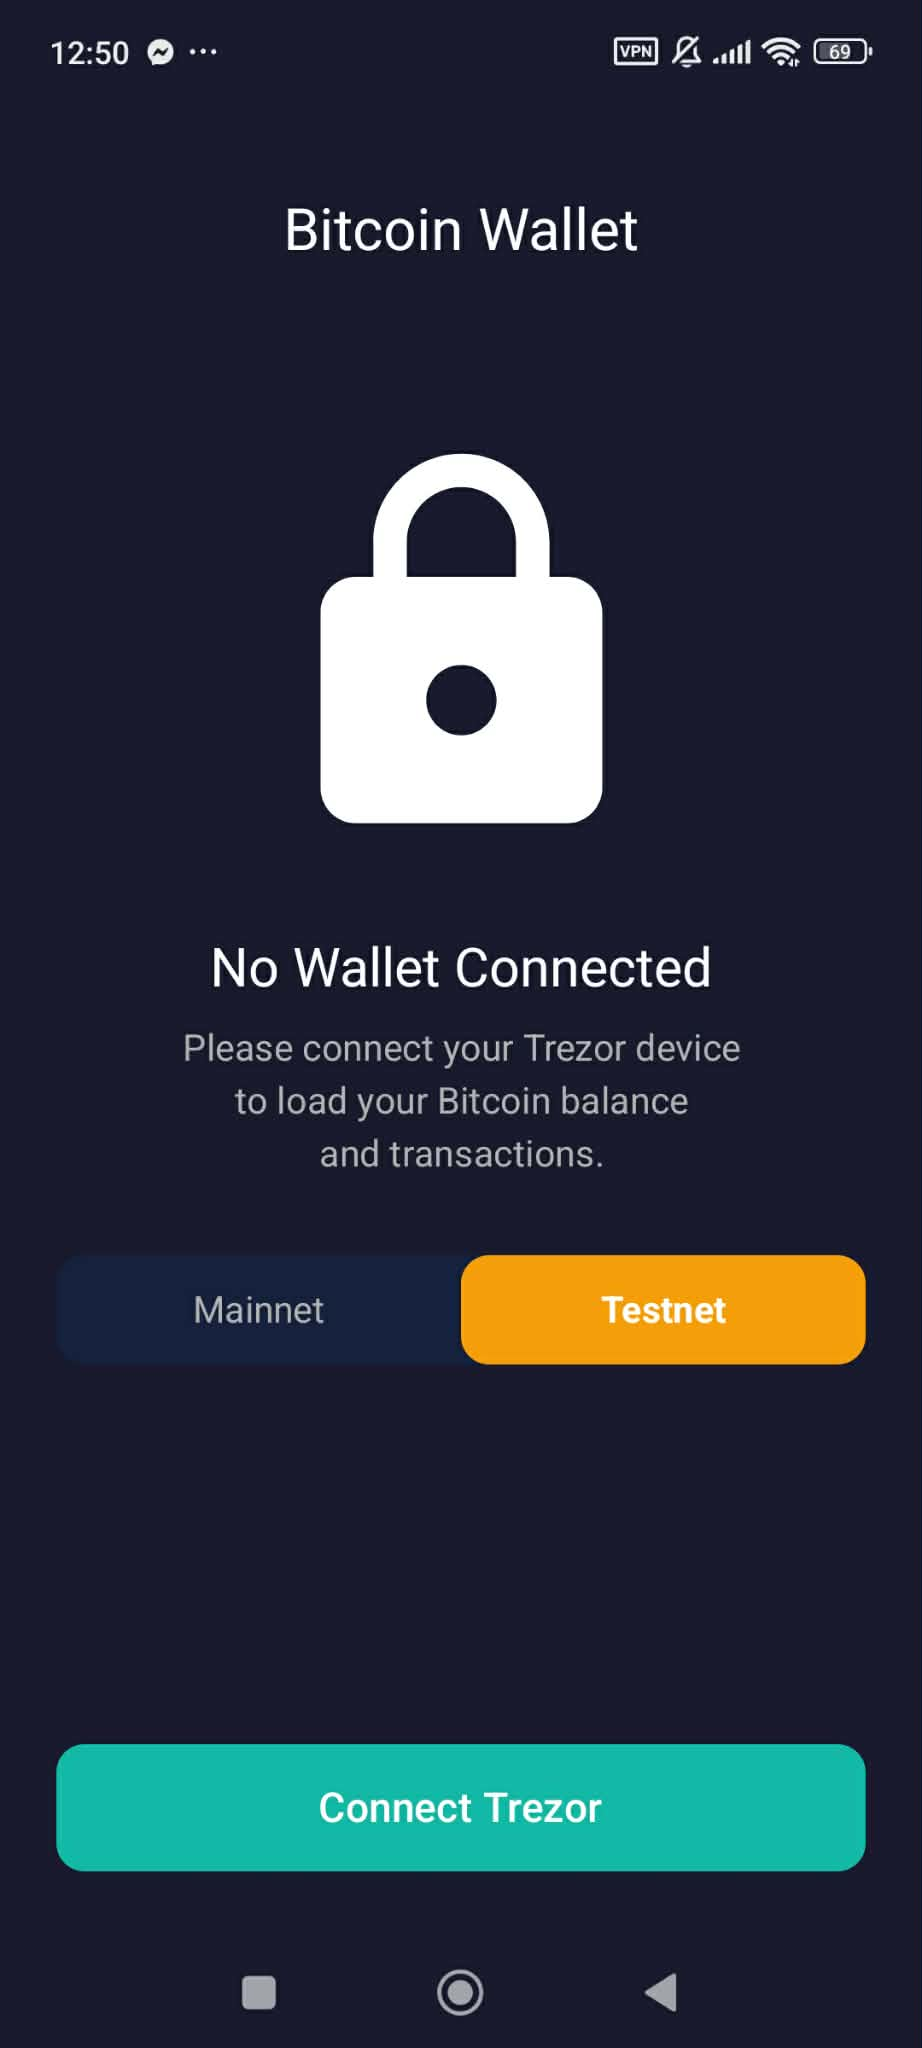
\includegraphics[height=0.3\textheight]{img/screen-login.jpeg}\hfill
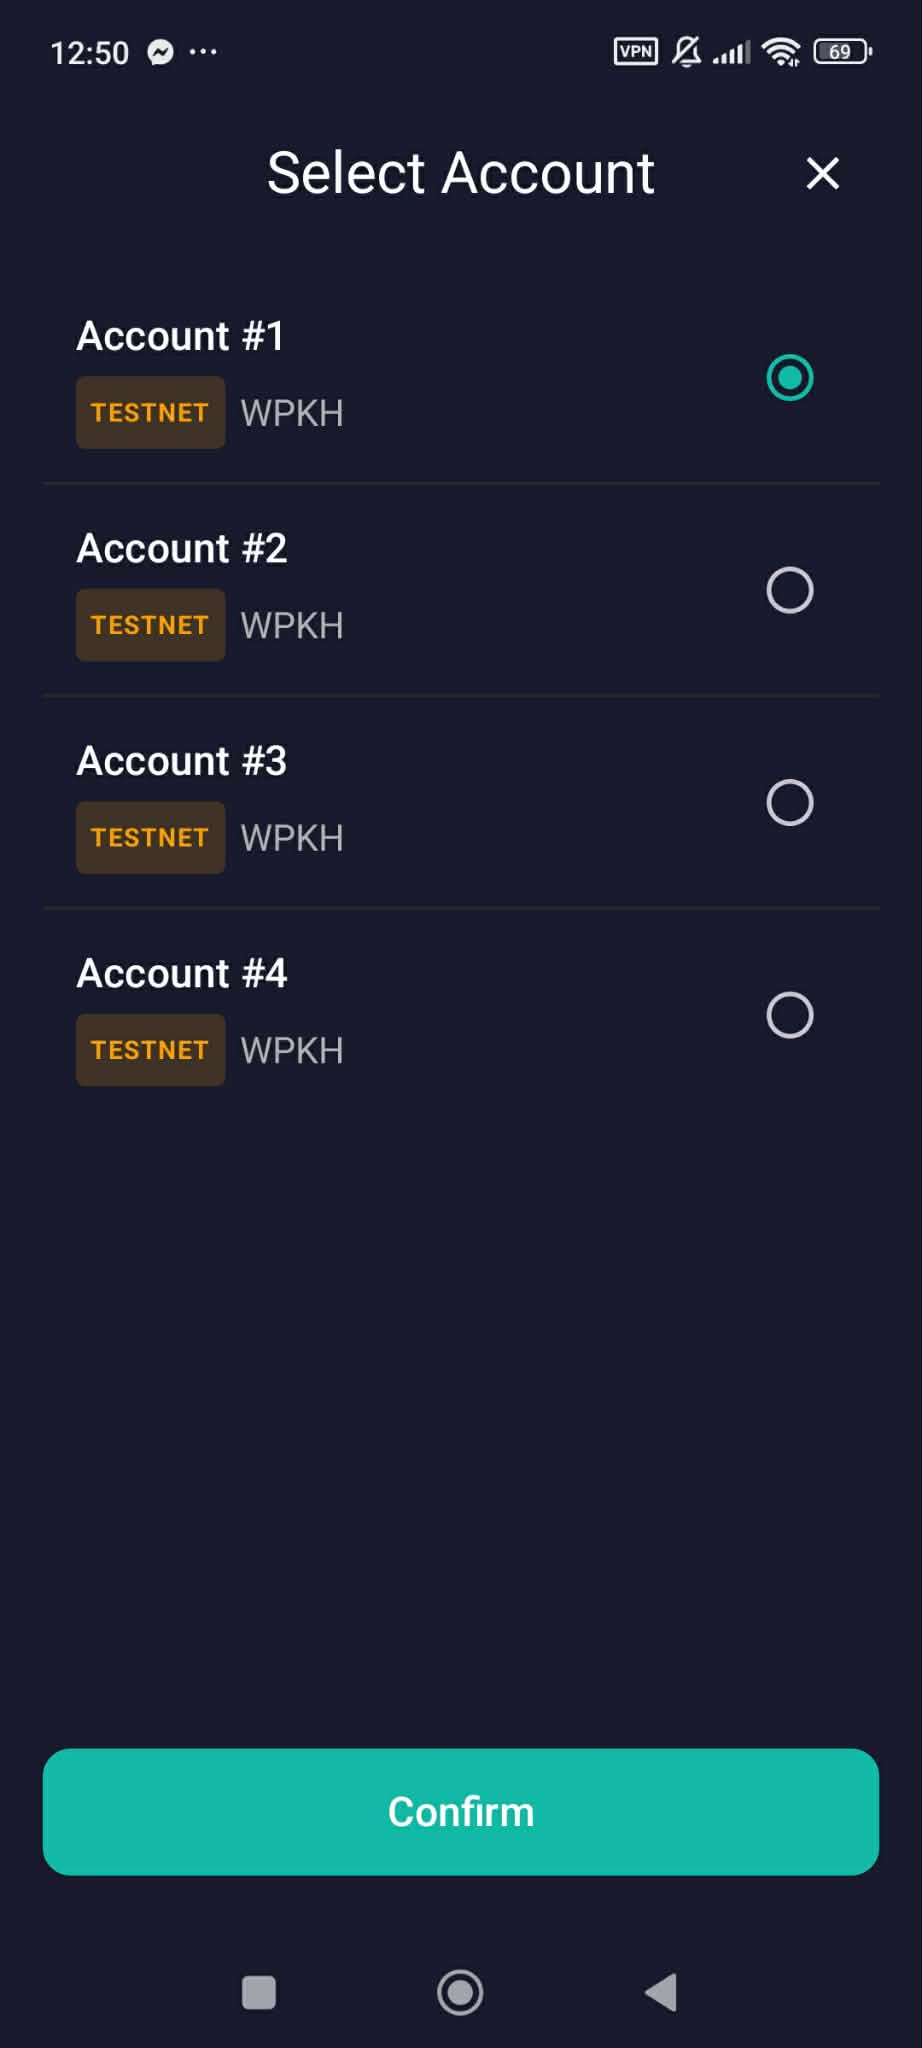
\includegraphics[height=0.3\textheight]{img/screen-select-account.jpeg}\hfill
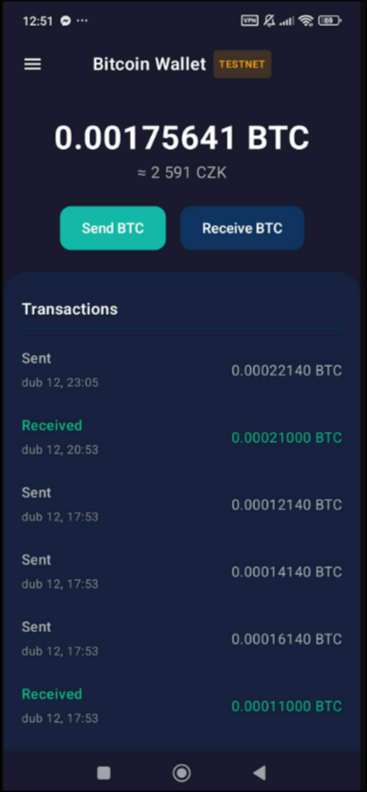
\includegraphics[height=0.3\textheight]{img/screen-dashboard.png}
\caption[Průběh přihlášení]{Průběh přihlášení. Vlevo: přihlašovací
obrazovka s~přepínačem sítě. Uprostřed: výběr singlesig účtu --
backend nalezl čtyři účty s~historií. Vpravo: hlavní obrazovka
(dashboard) se zůstatkem v~BTC a~CZK, seznamem transakcí a~tlačítky
pro odeslání a~příjem.}
\label{fig:screen-onboarding}
\end{figure}

Tento postup probíhá pouze při prvním přihlášení. V~běžném provozu
aplikace po~vypršení krátkodobého přístupového tokenu automaticky vymění
uchovávaný refresh token za~novou dvojici tokenů, aniž by uživatel
musel znovu exportovat klíče z~Trezoru; mechanismus rotace popisujeme
v~sekci~\ref{subsec:refresh-token}.

Hlavní obrazovka (dashboard) zobrazuje aktuální zůstatek v~BTC a~jeho
ekvivalent ve zvolené fiat měně (CZK, USD nebo EUR -- volbu měny lze
změnit v~nastavení aplikace, viz sekci~\ref{sec:user-nastaveni}). Pod
zůstatkem se nachází chronologický seznam transakcí seřazený od nejnovější;
u~každé transakce je uvedena částka, směr (odeslaná/přijatá), datum a~čas
nebo příznak \emph{Unconfirmed} u~dosud nepotvrzených transakcí. V~dolní části
obrazovky jsou dvě hlavní tlačítka: \emph{Send BTC} pro vytvoření nové
transakce a~\emph{Receive BTC} pro zobrazení přijímací adresy. V~levém
horním rohu ikona hamburgeru otevírá postranní navigační menu
(\emph{drawer}), které umožňuje přechod na seznam multisig peněženek
a~do nastavení. Kliknutím na konkrétní transakci v~seznamu se otevře její
detail (viz sekci~\ref{sec:user-detail-tx}).

%%% -----------------------------------------------------------------------
\section{Příjem prostředků}
\label{sec:user-prijem}

Po stisknutí \emph{Receive BTC} aplikace zobrazí aktuální přijímací adresu
(obrázek~\ref{fig:screen-receive}) ve formě řetězce \texttt{tb1q\ldots}
(na testnetu) nebo \texttt{bc1q\ldots} (na mainnetu) spolu
s~odpovídajícím QR kódem ve formátu BIP-21~\cite{BIP21} (URI ve tvaru
\texttt{bitcoin:<adresa>}). Adresu lze zkopírovat do schránky stisknutím
příslušného tlačítka.

Tlačítko \emph{Show On Trezor} umožňuje ověřit zobrazenou adresu přímo
na displeji hardwarové peněženky. Aplikace prostřednictvím deeplinku zavolá
metodu \texttt{getAddress} protokolu Trezor Connect~\cite{TrezorConnect}
a~Trezor na svém displeji zobrazí adresu odvozenou ze svých interních klíčů.
Uživatel vizuálně porovná obě adresy a~tím ověří, že aplikace nezobrazuje
podvrženou adresu. Tato funkce je dostupná jak pro singlesig, tak pro
multisig peněženky.

\begin{figure}[htbp]
\centering
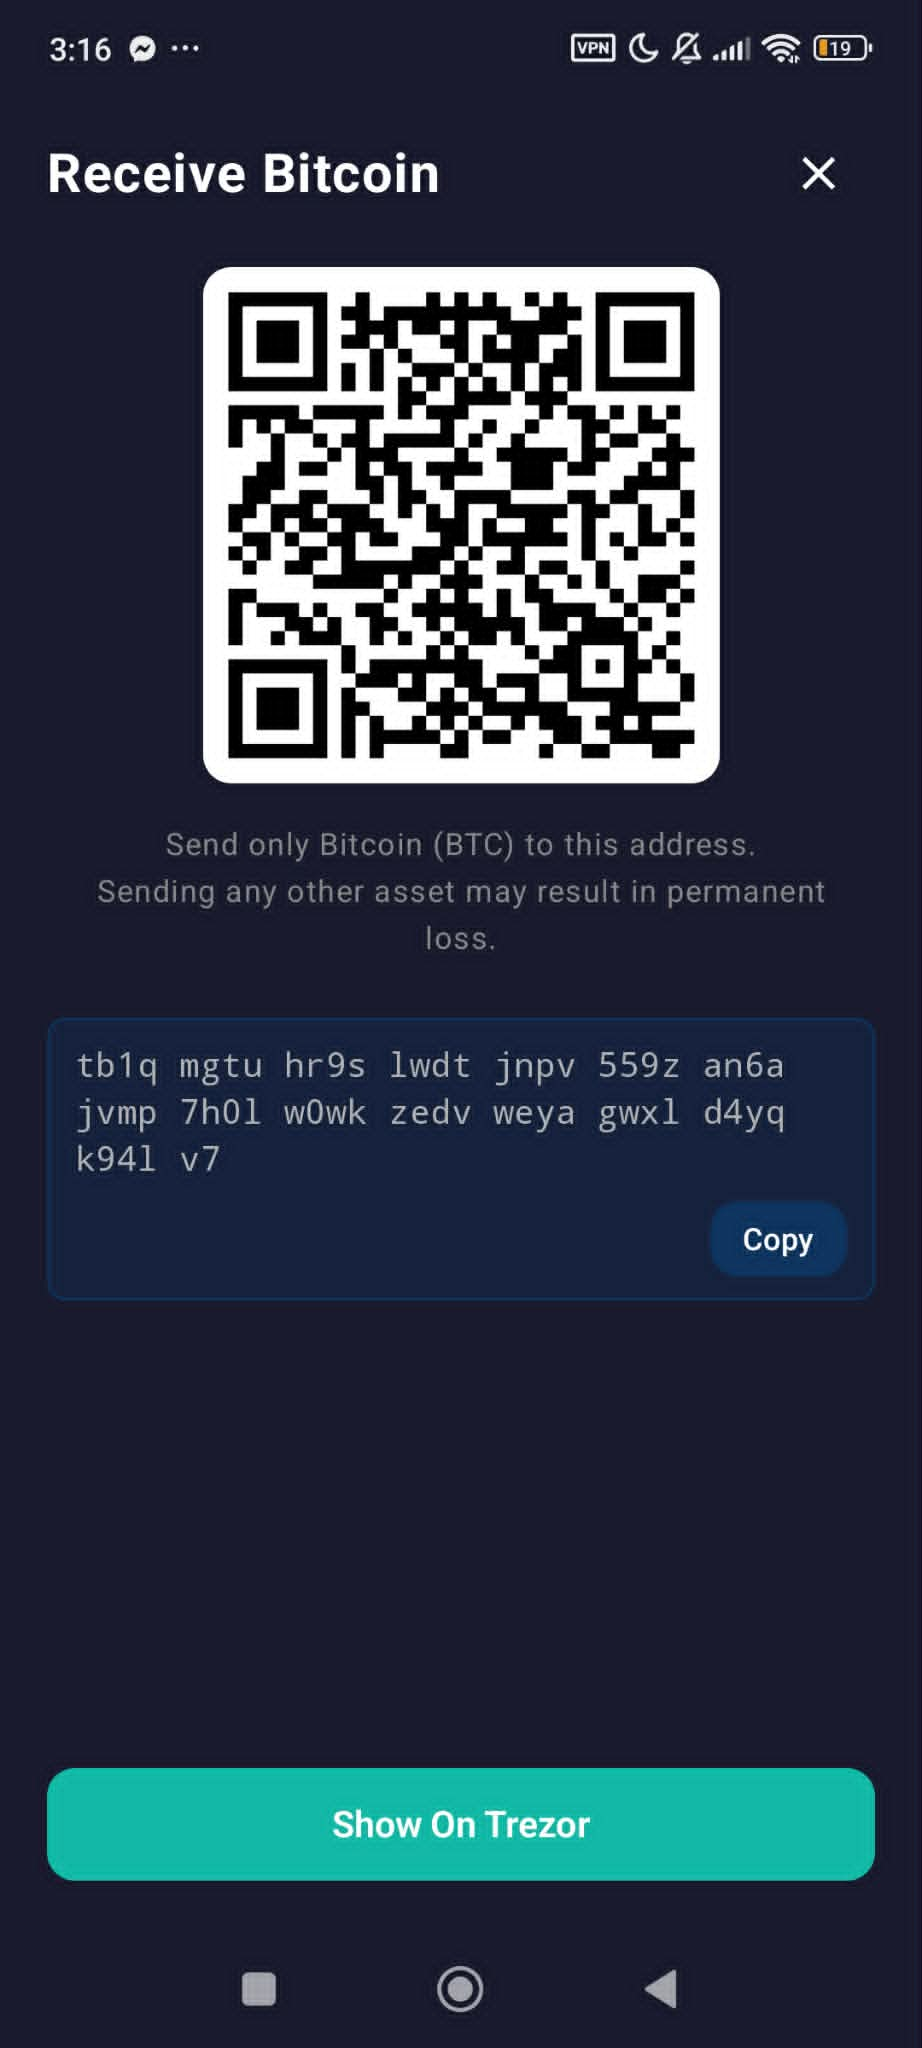
\includegraphics[height=0.3\textheight]{img/screen-receive.jpeg}
\caption[Příjem prostředků]{Příjem prostředků -- QR kód ve formátu
BIP-21, adresa s~možností kopírování a~tlačítko pro ověření adresy
na displeji Trezoru.}
\label{fig:screen-receive}
\end{figure}

Po přijetí prostředků na zobrazenou adresu se zůstatek
v~aplikaci aktualizuje po obnovení dashboardu; první potvrzení v~bloku
obvykle trvá 10--30 minut.

%%% -----------------------------------------------------------------------
\section{Odeslání singlesig transakce}
\label{sec:user-singlesig}

Po stisknutí \emph{Send BTC} se otevře formulář
(obrázek~\ref{fig:screen-send}) s~následujícími poli:

\begin{description}
\item[Cílová adresa] -- uživatel ji zadá ručně, vloží ze schránky, nebo
  naskenuje pomocí QR kódu z~fotoaparátu zařízení stisknutím ikony QR skeneru
  vedle pole adresy. Skener rozpozná jak prosté adresy, tak BIP-21
  URI~\cite{BIP21} ve tvaru \texttt{bitcoin:<adresa>} a~automaticky extrahuje
  samotnou adresu.

\item[Částka] -- zadává se v~BTC.

\item[Výběr UTXO] -- uživatel volí mezi automatickým výběrem (strategie
  \emph{largest-first}, viz sekci~\ref{subsec:coin-control}) a~manuálním
  výběrem (obrázek~\ref{fig:screen-send}, uprostřed). Při zvolení
  manuálního režimu se tlačítkem \emph{Edit} otevře obrazovka coin control
  (viz sekci~\ref{sec:user-coin-control}).

\item[Úroveň poplatku] -- výběr ze tří úrovní (nízký, střední, vysoký)
  s~aktuální sazbou v~sat/vB získanou z~mempoolu. V~manuálním režimu
  výběru UTXO je navíc dostupné pole pro zadání libovolné sazby ručně.
\end{description}

Pod formulářem se zobrazuje souhrn transakce: odesílaná částka, odhadovaný
poplatek, celková hodnota, aktuální zůstatek, prostředky rezervované
v~rozpracovaných PSBT (pokud existují) a~zbývající změna (change). Tím má
uživatel před potvrzením kompletní přehled o~dopadu transakce na svůj
zůstatek.

\begin{figure}[htbp]
\centering
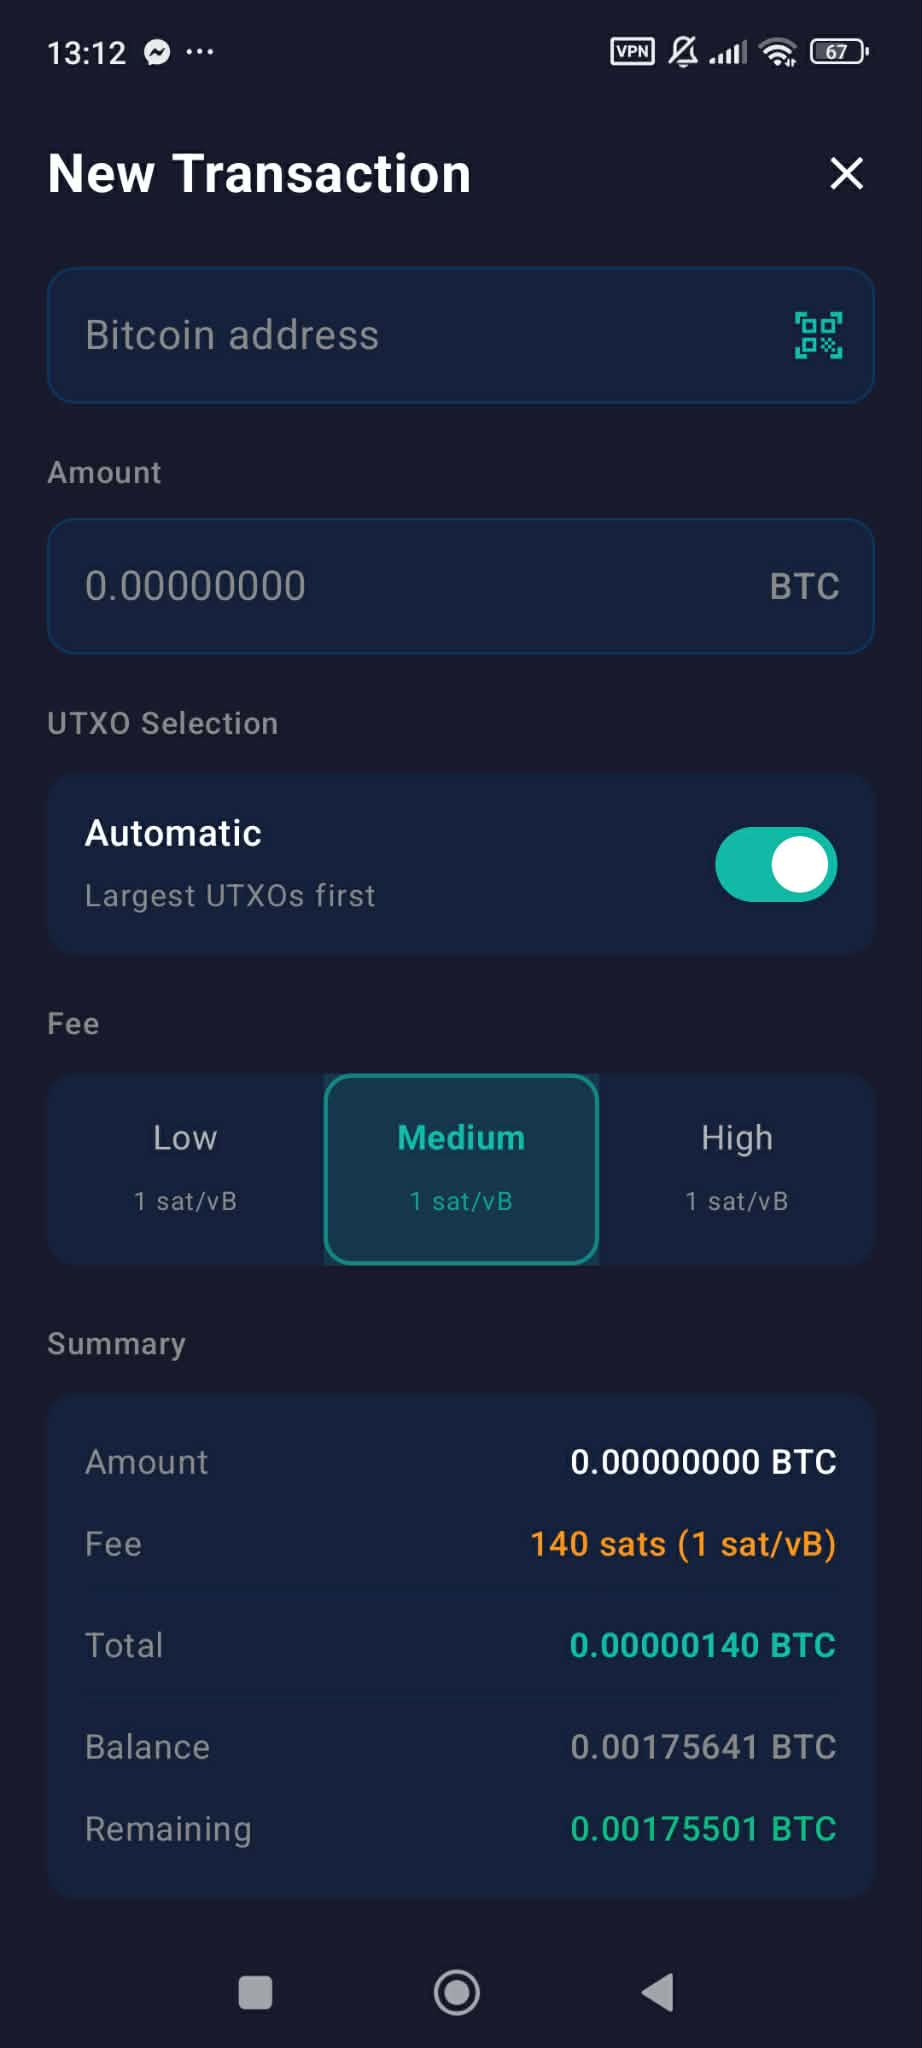
\includegraphics[height=0.3\textheight]{img/screen-send.jpeg}\hfill
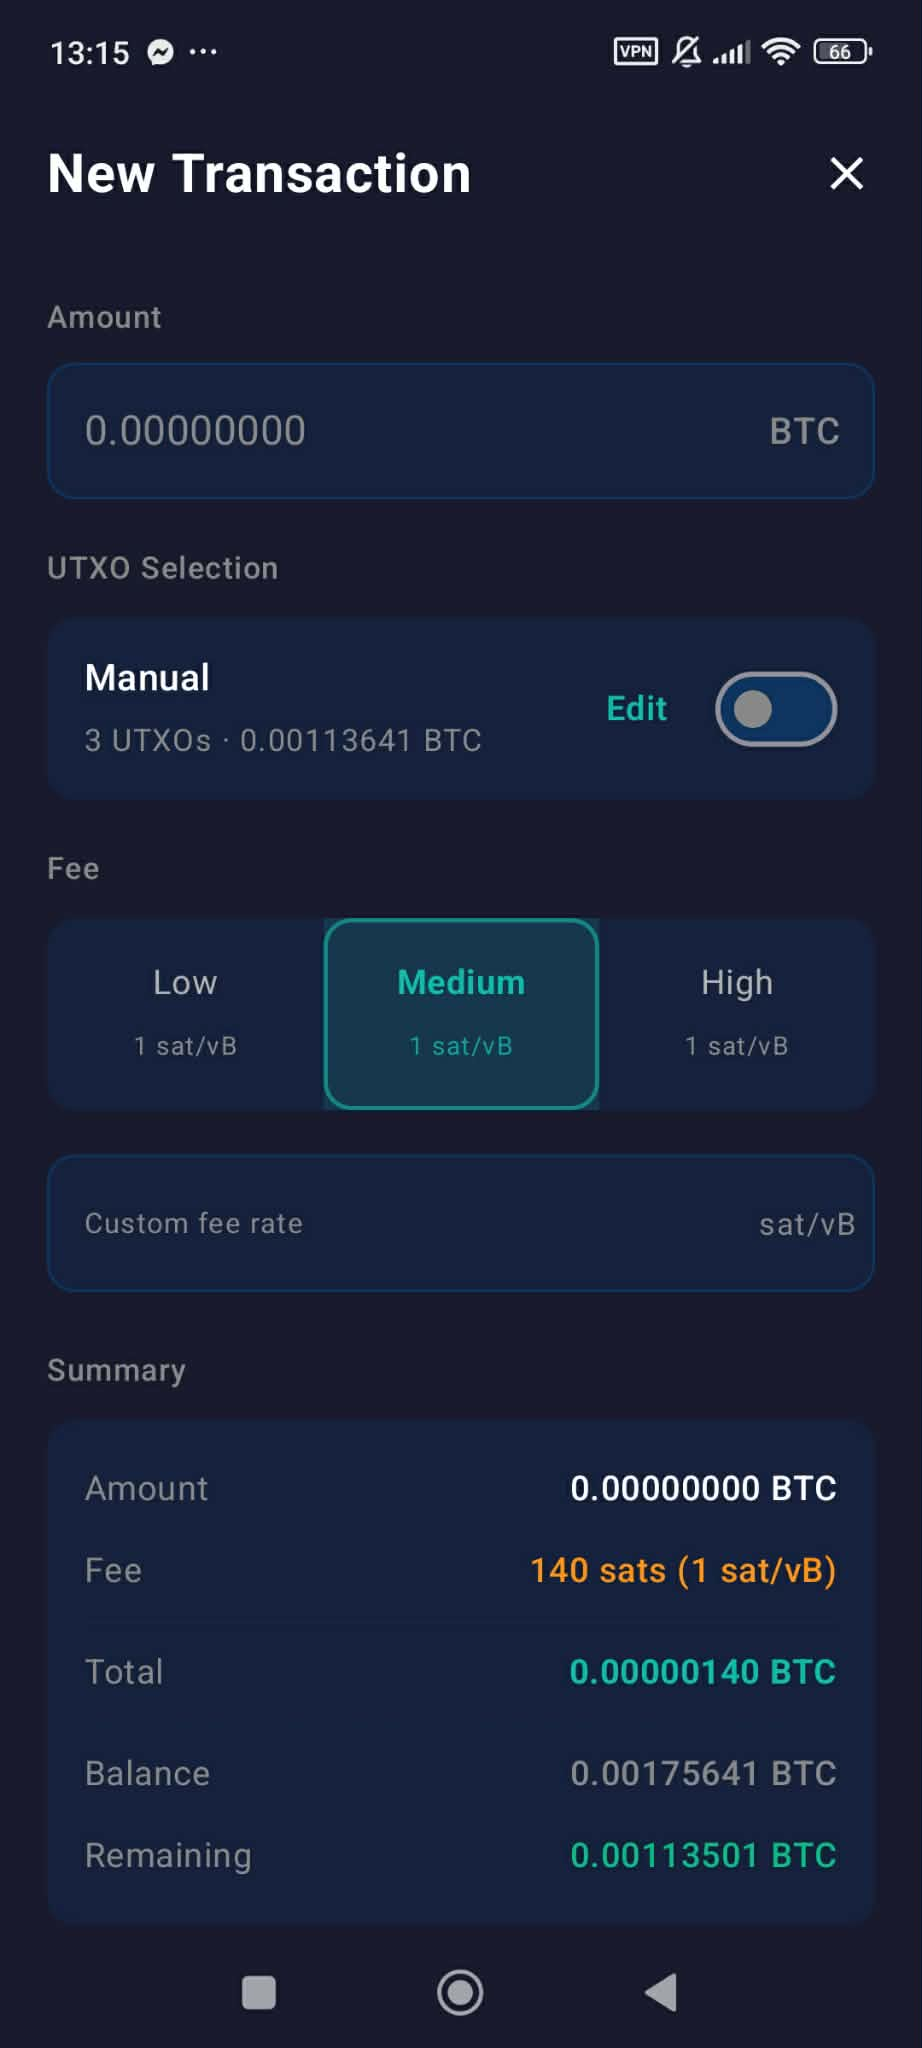
\includegraphics[height=0.3\textheight]{img/screen-send-manual.jpeg}\hfill
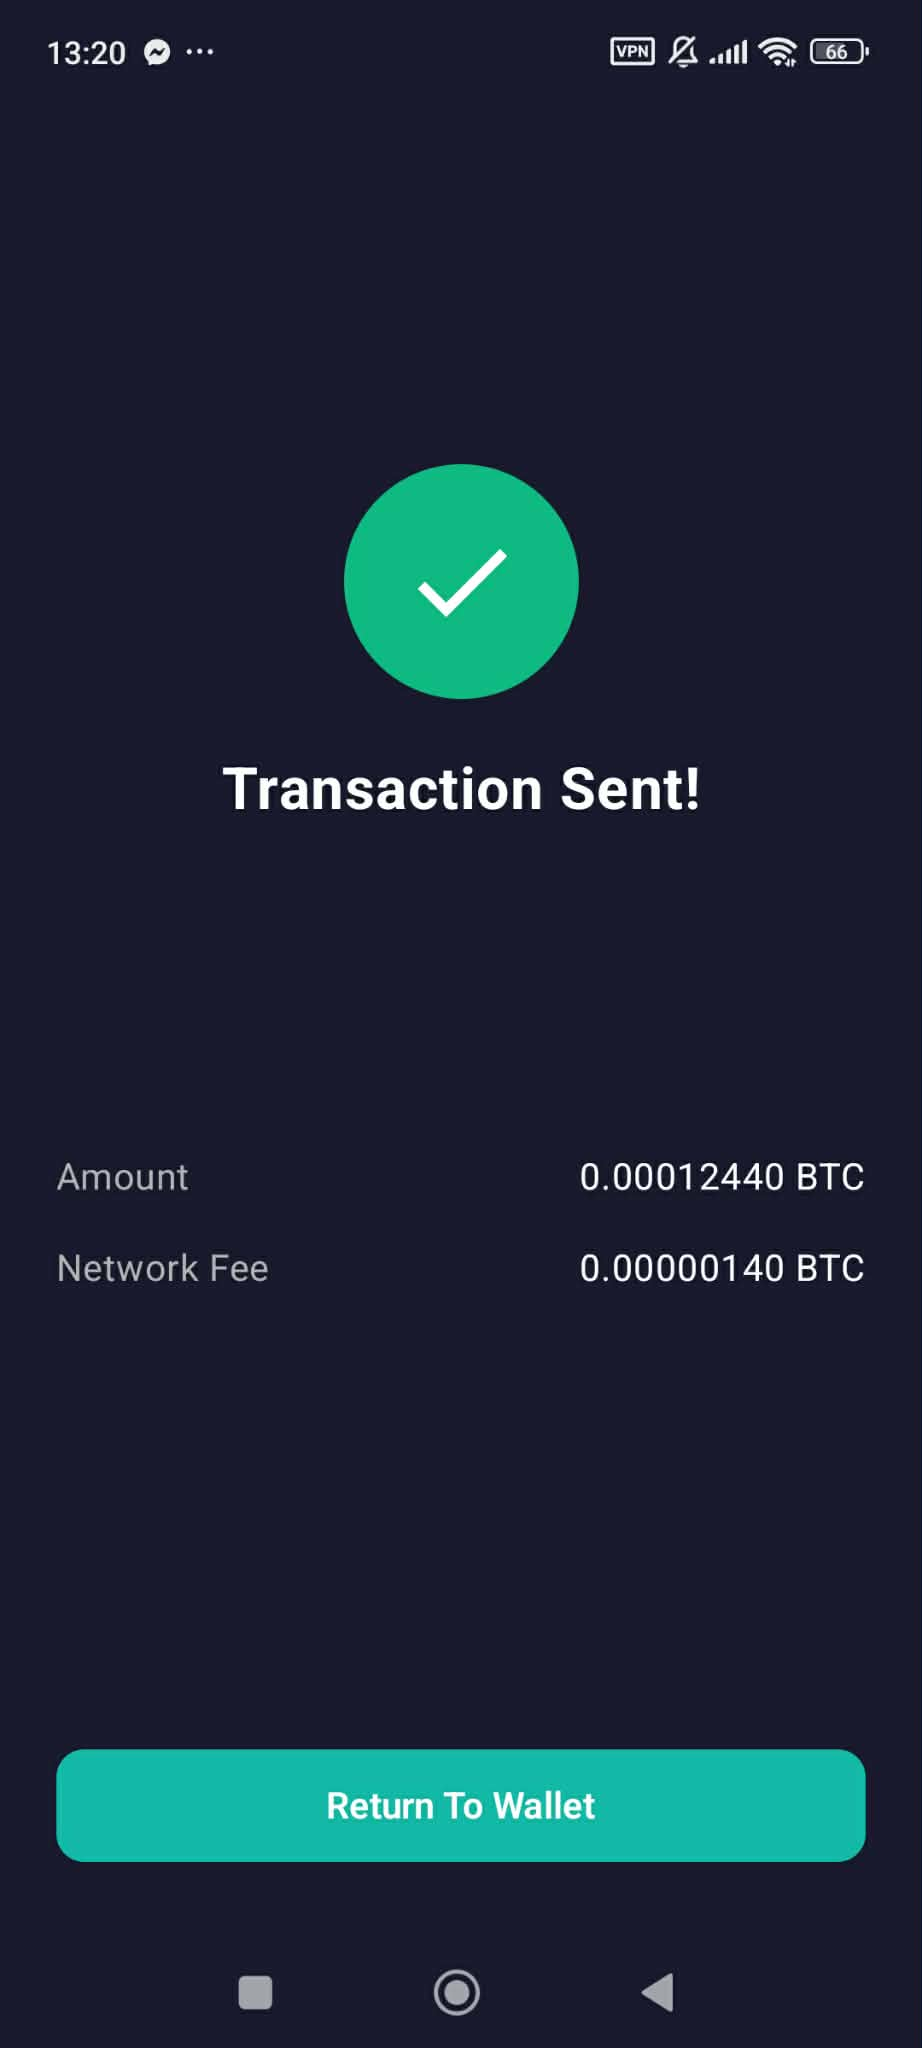
\includegraphics[height=0.3\textheight]{img/screen-tx-sent.jpeg}
\caption[Odeslání transakce]{Odeslání transakce. Vlevo: formulář
s~automatickým výběrem UTXO a~třemi úrovněmi poplatku. Uprostřed:
manuální režim s~počtem vybraných UTXO a~polem pro vlastní sazbu
v~sat/vB. Vpravo: potvrzení úspěšného odeslání se souhrnem částky
a~poplatku.}
\label{fig:screen-send}
\end{figure}

Po potvrzení odeslání backend sestaví transakci typu P2WPKH a~aplikace
přes deeplink přesměruje uživatele do Trezor Suite Mobile. Tam se
na displeji hardwarové peněženky zobrazí cílová adresa, částka a~poplatek
ke kontrole; uživatel podpis fyzicky potvrdí stisknutím tlačítka na
zařízení. Trezor vrátí kompletní podepsanou transakci, kterou aplikace
předá backendu k~broadcastu do Bitcoinové sítě. Po úspěšném broadcastu
aplikace zobrazí potvrzení s~částkou a~poplatkem
(obrázek~\ref{fig:screen-send}, vpravo),
podle kterého lze průběh sledovat v~kterémkoli prohlížeči blockchainu.
V~případě neúspěchu (například odmítnutí podpisu na Trezoru nebo chyba
sítě) se zobrazí chybová obrazovka s~popisem problému a~tlačítkem pro
návrat na dashboard.

%%% -----------------------------------------------------------------------
\section{Manuální výběr UTXO (coin control)}
\label{sec:user-coin-control}

Obrazovka coin control (obrázek~\ref{fig:screen-tools}, vlevo) zobrazuje
seznam všech nepoužitých výstupů (UTXO) aktuální peněženky. U~každého UTXO
je uvedena částka v~BTC, adresa, datum vytvoření a~stav:

\begin{description}
\item[Potvrzený] (zelený příznak) -- UTXO je potvrzeno v~alespoň jednom
  bloku a~je k~dispozici pro výběr.
\item[Nepotvrzený] (žlutý příznak) -- UTXO pochází z~transakce, která
  dosud nebyla zařazena do bloku. Je k~dispozici pro výběr, ale transakce
  využívající nepotvrzený vstup může být zpožděna.
\item[Rezervovaný] (červený příznak) -- UTXO je zamčeno v~rozpracované
  PSBT transakci čekající na podpisy. Takové UTXO nelze vybrat, aby se
  předešlo dvojímu utracení.
\end{description}

Uživatel zaškrtne konkrétní UTXO, která chce použít jako vstupy transakce.
V~horní části obrazovky se průběžně zobrazuje počet vybraných UTXO
a~jejich celková hodnota. Tlačítkem \emph{Order By} je možné změnit řazení
seznamu podle hodnoty, data, stavu potvrzení nebo adresy.

Kliknutím na obsah řádku UTXO (nikoliv na zaškrtávací pole) se otevře
detail příslušné transakce (viz sekci~\ref{sec:user-detail-tx}), kde
uživatel může prozkoumat původ prostředků.

%%% -----------------------------------------------------------------------
\section{Detail transakce}
\label{sec:user-detail-tx}

Obrazovka detailu transakce (obrázek~\ref{fig:screen-tools}, uprostřed)
zobrazuje kompletní informace o~zvolené transakci: stav potvrzení
(potvrzená s~výškou bloku, nebo nepotvrzená), časové razítko, poplatek
v~BTC, sazbu poplatku v~sat/vB a~velikost transakce v~bajtech.

Pod hlavičkou se nachází dva seznamy: vstupy a~výstupy transakce. U~každého
vstupu a~výstupu je zobrazena adresa, hodnota v~BTC a~barevné příznaky:
\emph{YOURS} označuje adresu patřící aktuální peněžence a~\emph{FROM HERE}
zvýrazňuje výstup, z~něhož uživatel na tuto transakci přišel (při
rekurzivním procházení). Kliknutím na vstup nebo výstup se otevře detailní
dialog zobrazující plnou adresu, hodnotu v~BTC i~v~satoshi a~v~případě
vstupu i~identifikátor předchozí transakce s~tlačítkem
\emph{Open previous transaction}.

Tímto tlačítkem uživatel otevře předchozí transakci odpovídající danému
vstupu, čímž může rekurzivně sledovat původ prostředků. Aktuální hloubku
průchodu zobrazuje indikátor v~záhlaví (například \uv{Depth 2~/~5}). Aby
nedošlo k~nadměrnému zatížení blockchainového API, je hloubka průchodu
omezena na pět úrovní; po dosažení limitu se zobrazí upozornění. Tlačítko
\emph{Zavřít} v~horní části obrazovky vrátí uživatele zpět na dashboard
bez ohledu na aktuální hloubku průchodu.

\begin{figure}[htbp]
\centering
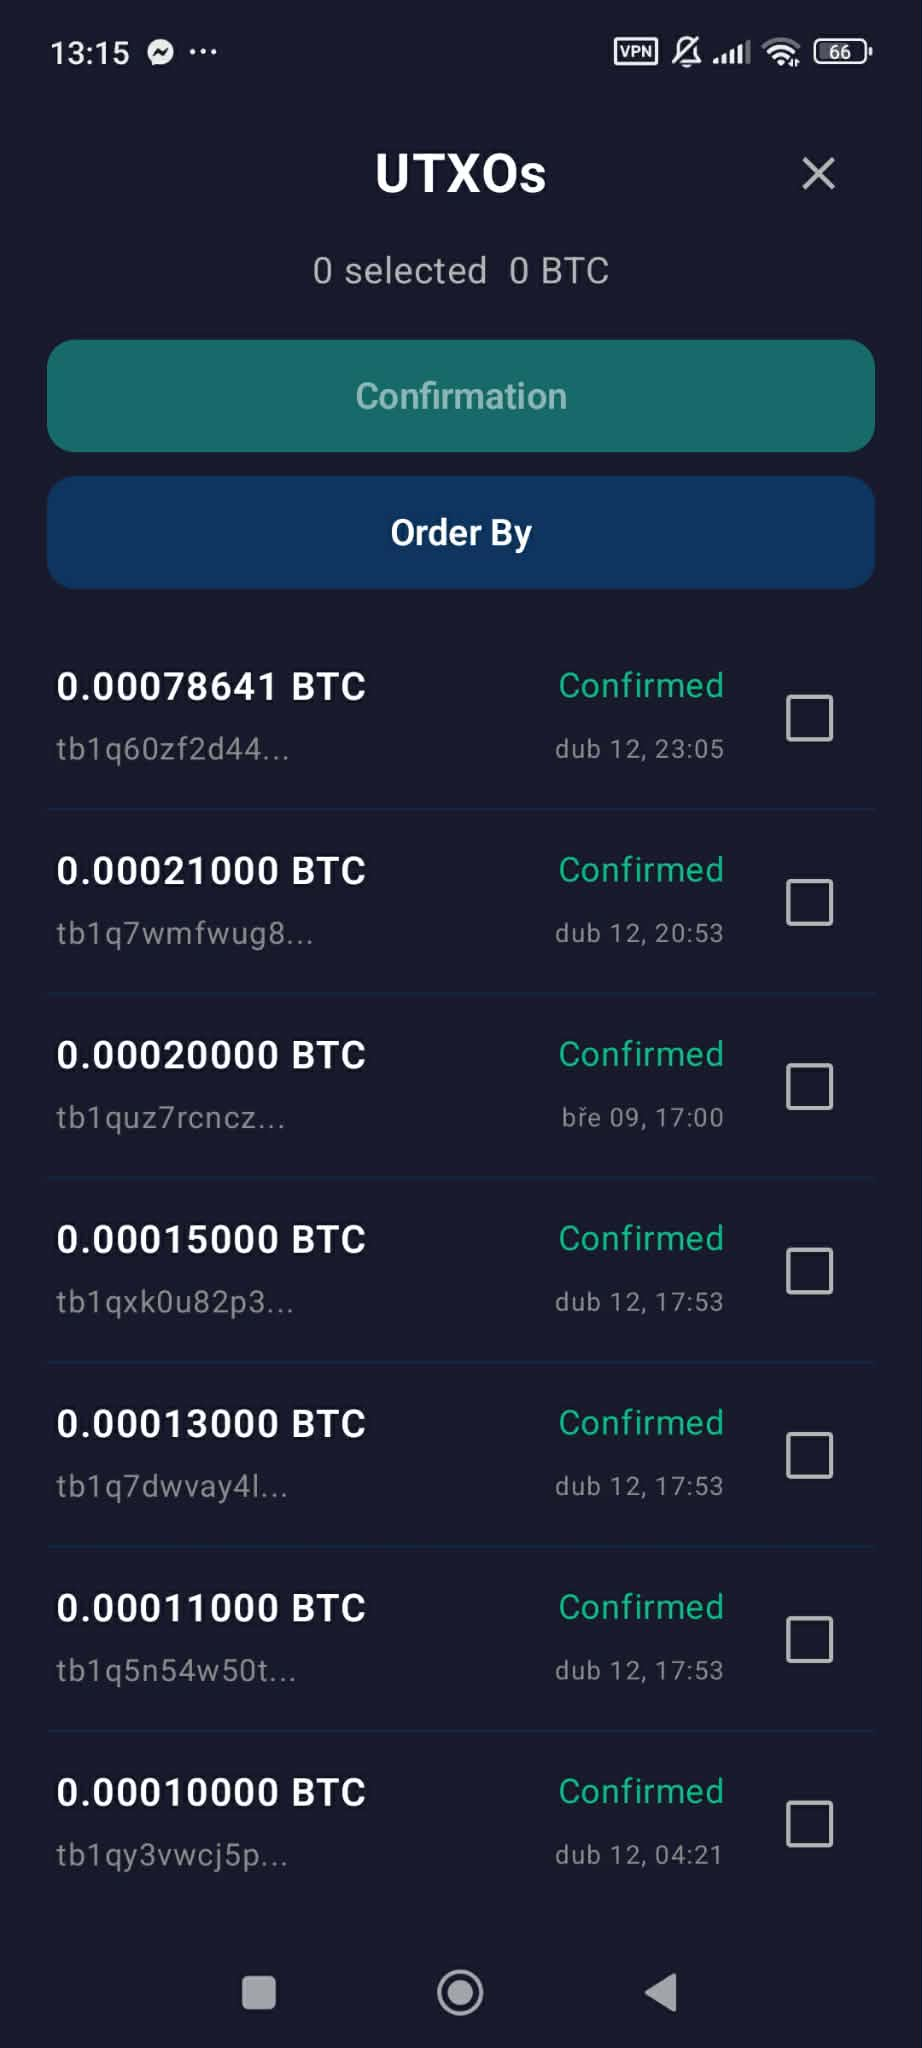
\includegraphics[height=0.3\textheight]{img/screen-coin-control.jpeg}\hfill
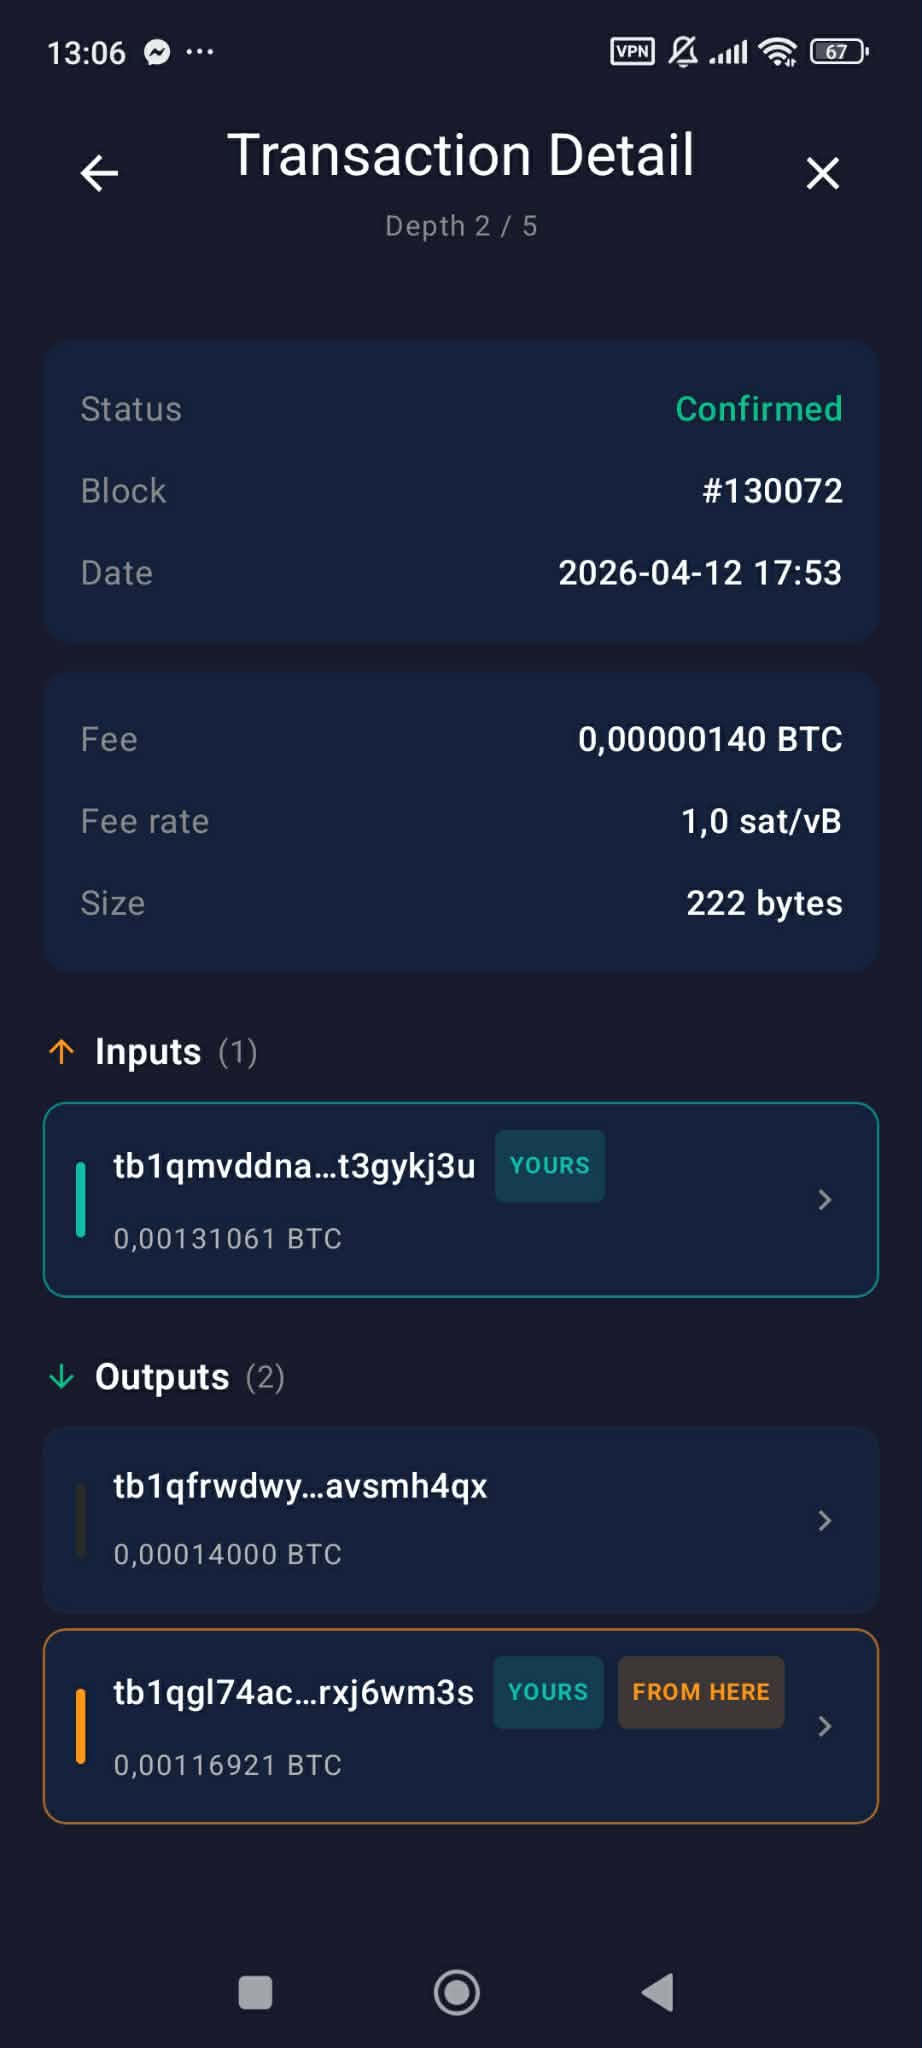
\includegraphics[height=0.3\textheight]{img/screen-tx-detail.jpeg}\hfill
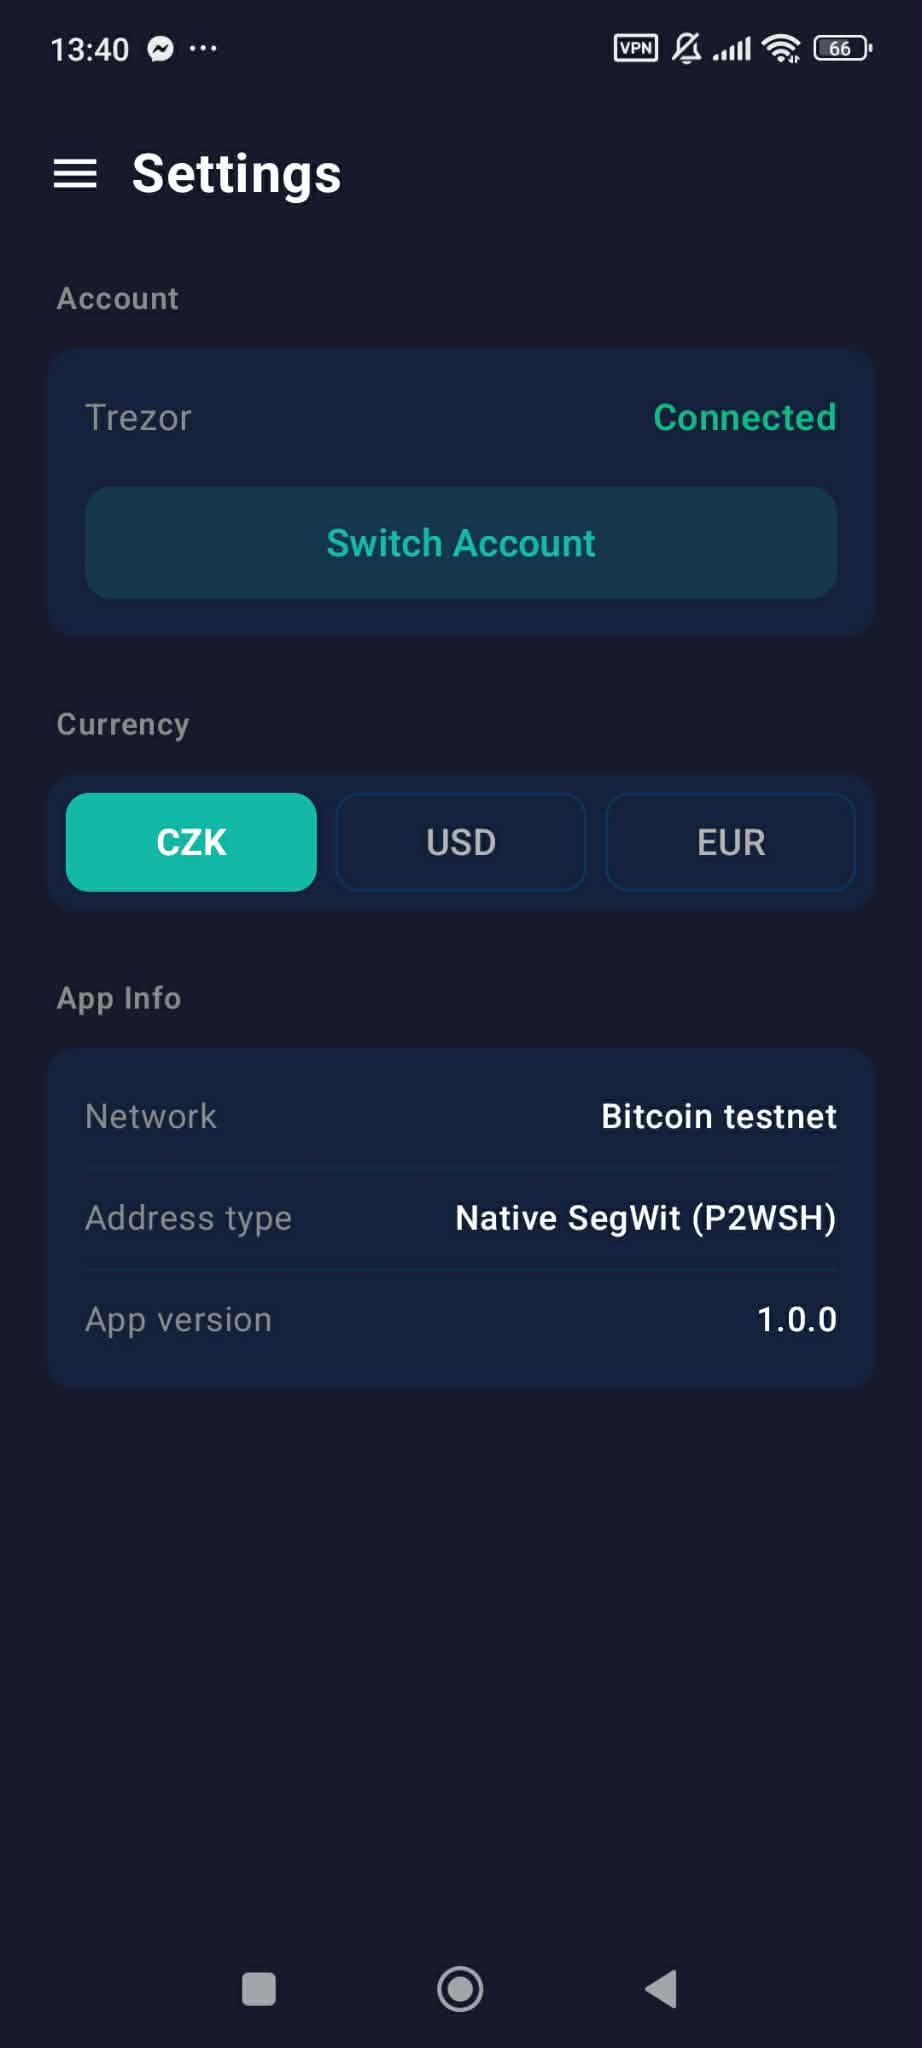
\includegraphics[height=0.3\textheight]{img/screen-settings.jpeg}
\caption[Coin control, detail transakce a nastavení]{Vlevo: coin
control -- seznam UTXO s~hodnotou, adresou, datem a~stavem potvrzení.
Uprostřed: detail transakce v~hloubce 2\,/\,5 s~příznaky \emph{YOURS}
a~\emph{FROM HERE}. Vpravo: nastavení -- přepnutí účtu, výběr fiat
měny a~informace o~aplikaci.}
\label{fig:screen-tools}
\end{figure}

%%% -----------------------------------------------------------------------
\section{Nastavení}
\label{sec:user-nastaveni}

Obrazovka nastavení (obrázek~\ref{fig:screen-tools}, vpravo) je přístupná
z~postranního navigačního menu a~obsahuje následující funkce:

\begin{description}
\item[Přepnout účet] -- smaže aktuální výběr peněženky a~přesměruje
  uživatele zpět na obrazovku výběru účtu. V~kontextu multisig testování
  (popsaného v~sekci~\ref{sec:user-multisig-podpis}) umožňuje přepínat
  mezi různými BIP-48 účty na témže Trezoru, čímž uživatel simuluje
  různé cosignery.

\item[Fiat měna] -- přepínač umožňující zvolit měnu pro zobrazení
  ekvivalentní hodnoty zůstatku: česká koruna (CZK), americký dolar (USD)
  nebo euro (EUR). Volba se projeví na dashboardu i~na detailu multisig
  peněženky. Směnný kurz je poskytován službou \texttt{price-service},
  která jej získává z~CoinGecko API~\cite{CoinGeckoAPI}.

\item[Informace o~aplikaci] -- zobrazuje síť (Bitcoin mainnet/testnet),
  typ adres (Native SegWit) a~verzi aplikace.
\end{description}

%%% -----------------------------------------------------------------------
\section{Multisig peněženky}
\label{sec:user-multisig}

Práce s~multisig peněženkou probíhá ve dvou fázích: jednorázový import
existujícího deskriptoru a~opakované podepisování konkrétních transakcí
postupně více cosignery.

\subsection{Import deskriptoru}
\label{sec:user-import}

Multisig peněženka se v~aplikaci vytvoří importem výstupního deskriptoru
ve formátu \texttt{wsh(sortedmulti(M,\ldots))} podle BIP-380~\cite{BIP380}
a~BIP-383~\cite{BIP383}. Deskriptor obsahuje práh~$M$, seznam xpub klíčů
všech cosignerů a~jejich derivační cesty. Podrobný popis formátu uvádíme
v~sekci~\ref{sec:descriptors}.

V~praxi předpokládáme, že deskriptor vytvoří jeden z~cosignerů
v~desktopové aplikaci -- nejčastěji Sparrow Wallet~\cite{SparrowWallet} --,
ze své instance Trezoru exportuje xpub a~od ostatních cosignerů obdrží
jejich xpub klíče stejným způsobem. Sparrow z~těchto klíčů vygeneruje
hotový deskriptor, který následně cosigneři předají všem členům multisig
peněženky (například skrze e-mail nebo sdílený dokument). Deskriptor
neobsahuje žádné soukromé údaje, takže jeho přenos nepředstavuje
bezpečnostní riziko.

V~mobilní aplikaci uživatel přejde z~postranního menu na seznam multisig
peněženek a~stiskne tlačítko \emph{Import Wallet}. Na importní obrazovce
(obrázek~\ref{fig:screen-multisig-setup}, vlevo) jsou k~dispozici dva
způsoby zadání deskriptoru:

\begin{enumerate}
\item \textbf{Vložení textu} -- uživatel zkopíruje deskriptor ze schránky
  do textového pole. Tento způsob je vhodný, pokud deskriptor obdržel
  například e-mailem nebo v~textové zprávě.

\item \textbf{Skenování QR kódu} -- stisknutím ikony QR skeneru vedle
  textového pole se otevře fotoaparát. Aplikace podporuje jak jednoduché
  QR kódy s~textovým deskriptorem, tak animované vícesnímkové QR kódy
  ve formátu UR (\emph{Uniform Resources})~\cite{BCR2020005}. Formát UR
  rozděluje dlouhá data do~sekvence menších QR kódů, které se postupně
  zobrazují na obrazovce zdrojového zařízení; aplikace je snímá
  průběžně a~zobrazuje ukazatel postupu (například \uv{Čtení QR\ldots{}
  65\,\%}). Tento formát používají airgap peněženky jako Keystone
  nebo Passport a~podporuje jej i~Sparrow Wallet pro export
  deskriptorů bez nutnosti síťového připojení.
\end{enumerate}

Volitelně může uživatel zadat pojmenování peněženky (například
\uv{Rodinná pokladna}). Backend deskriptor parsuje, odvodí přijímací
a~change adresy a~ověří jejich historii v~blockchainu. Po dokončení se nově
importovaná peněženka zobrazí v~seznamu multisig peněženek
(obrázek~\ref{fig:screen-multisig-setup}, uprostřed) s~označením prahu
(například \uv{2-of-3}) a~aktuálním zůstatkem.

\begin{figure}[htbp]
\centering
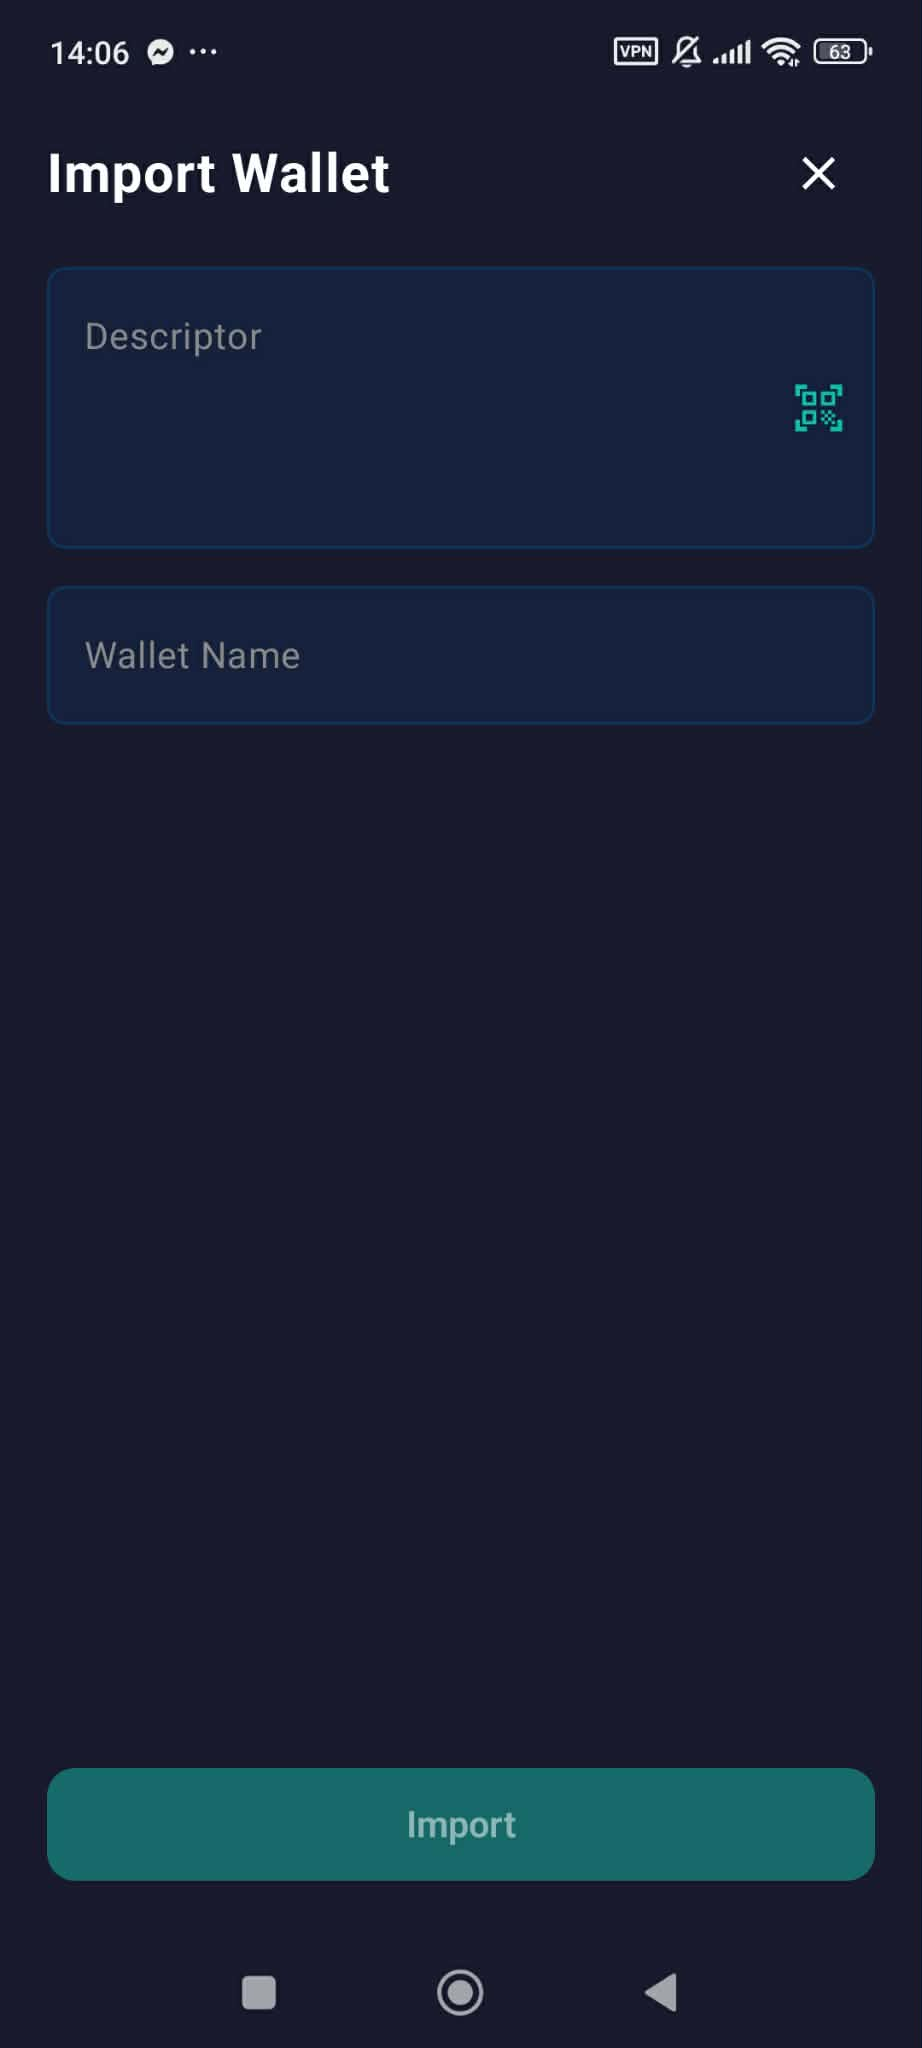
\includegraphics[height=0.3\textheight]{img/screen-import.jpeg}\hfill
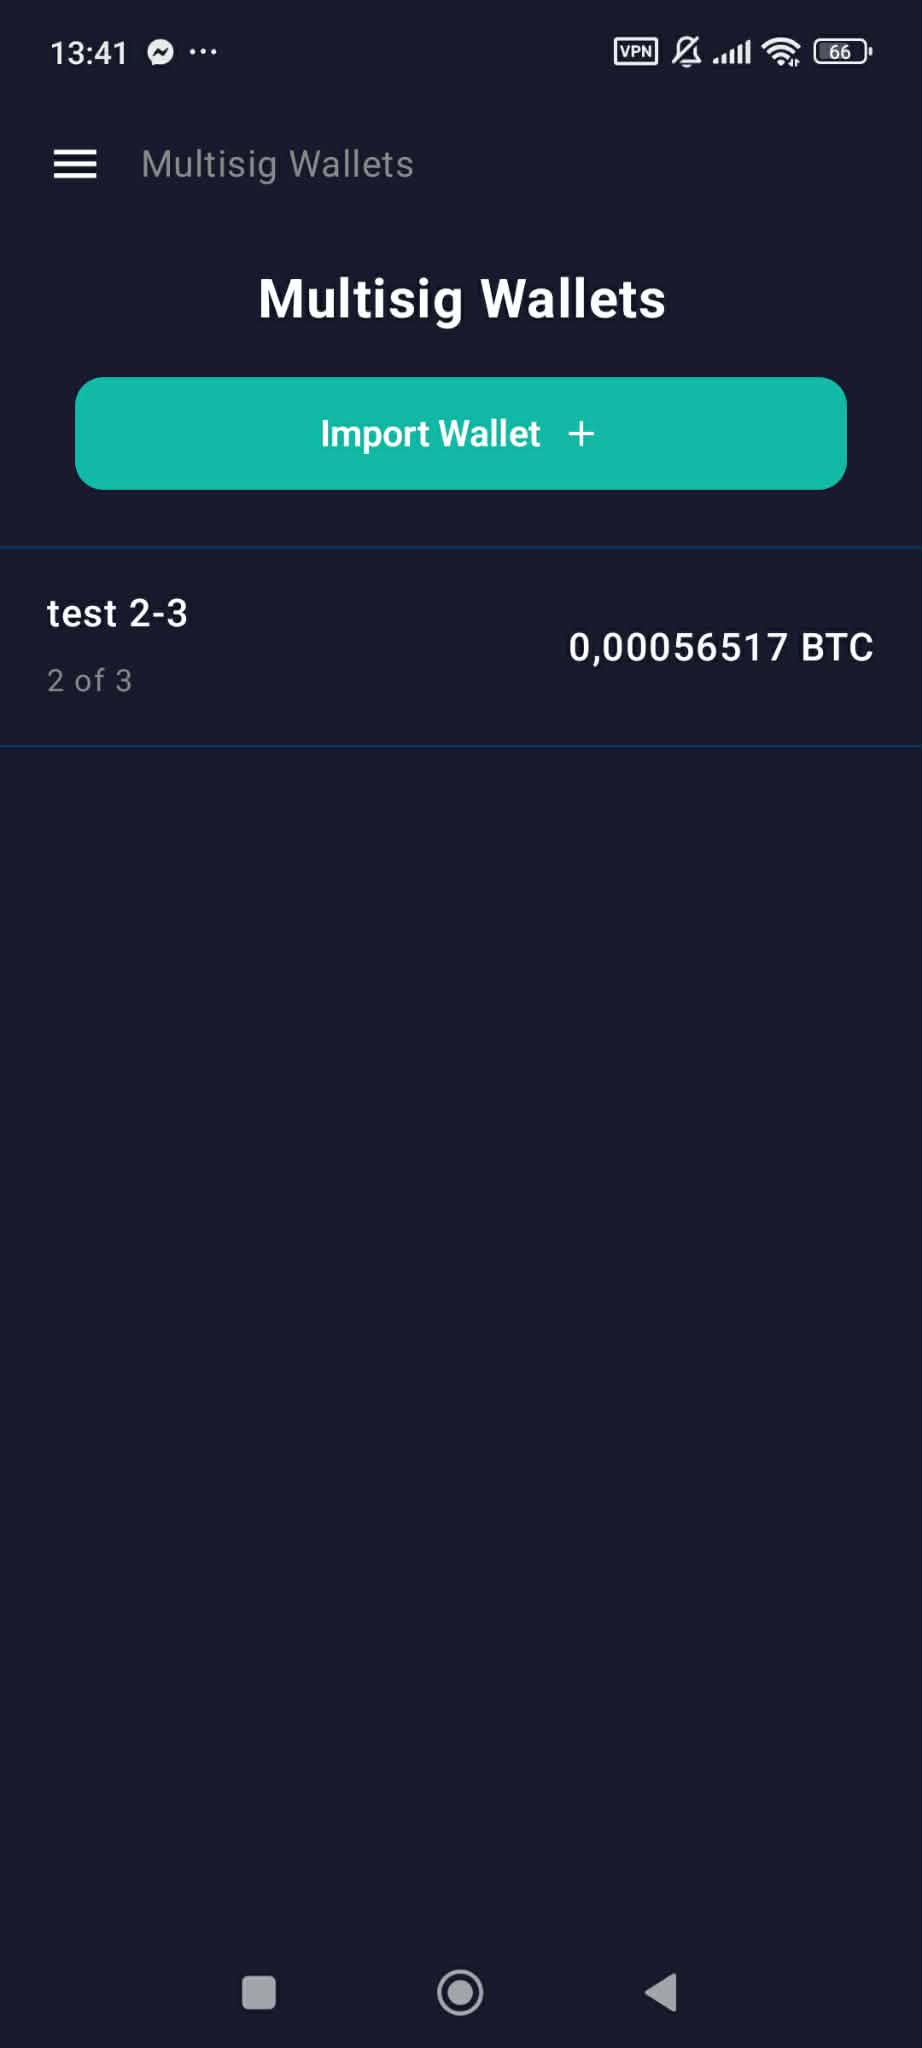
\includegraphics[height=0.3\textheight]{img/screen-multisig-list.jpeg}\hfill
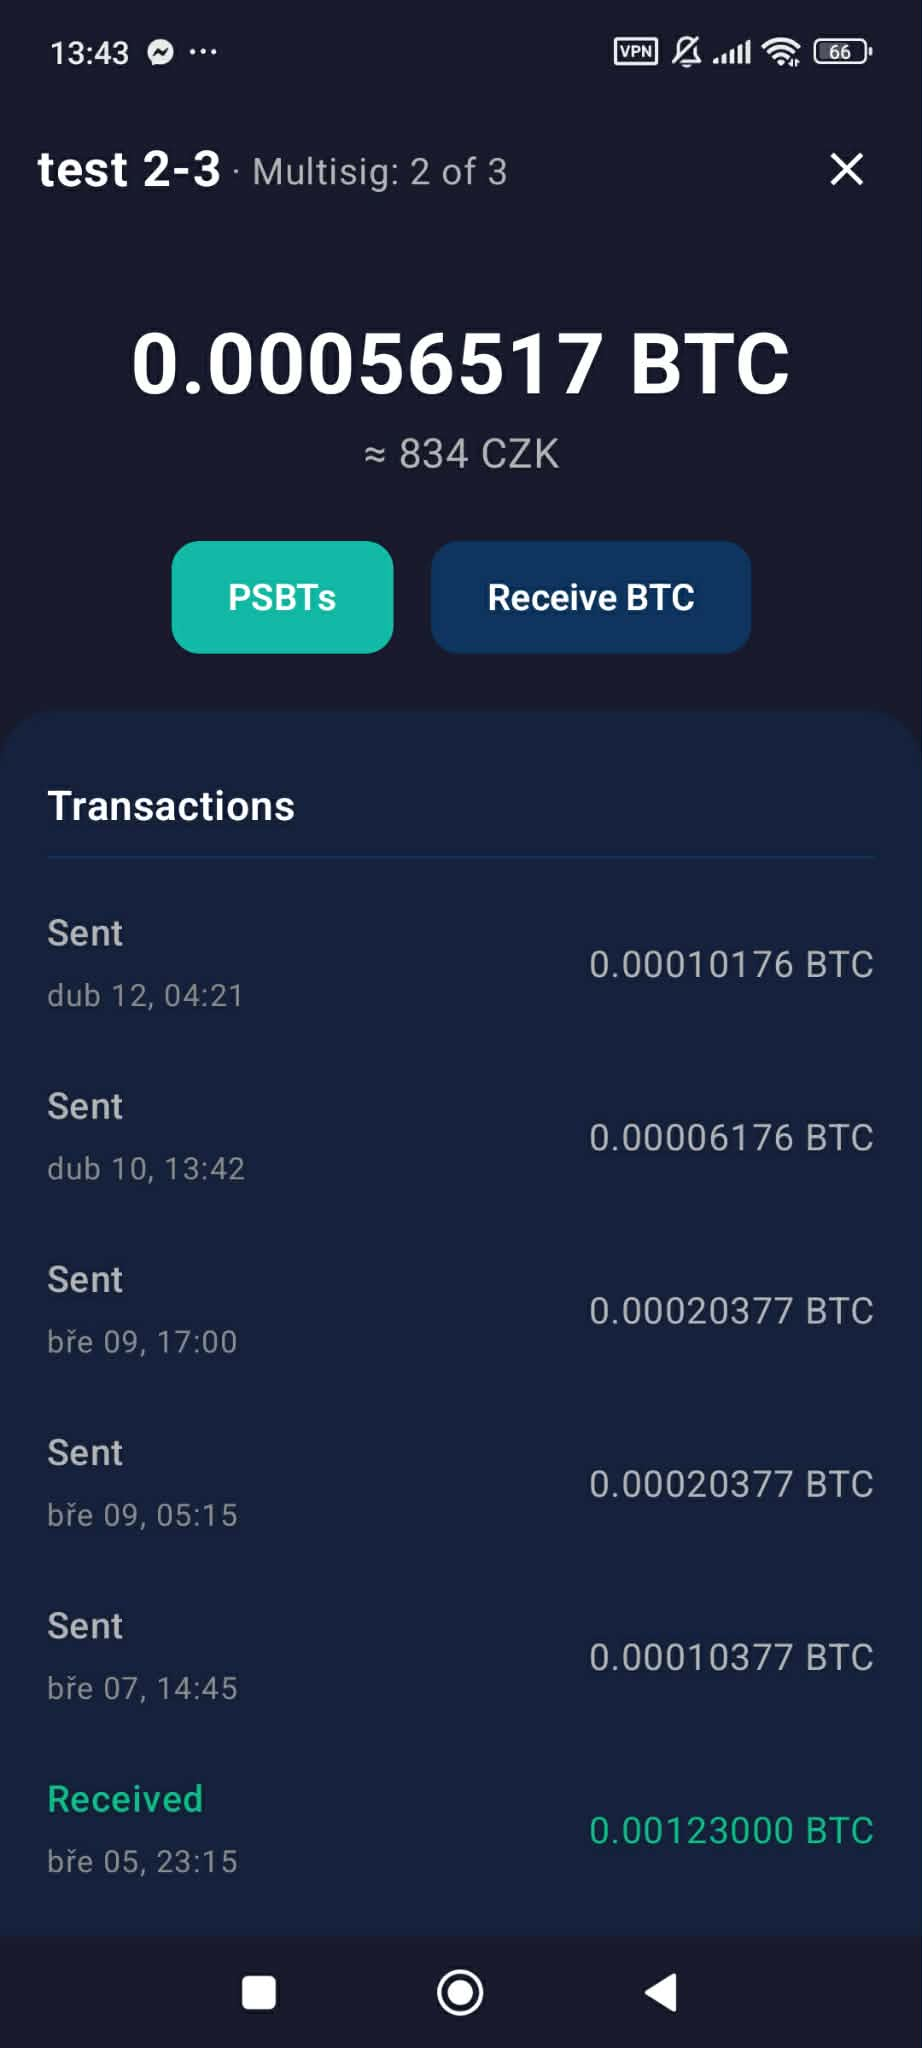
\includegraphics[height=0.3\textheight]{img/screen-multisig-detail.jpeg}
\caption[Multisig peněženky -- import a detail]{Multisig peněženky.
Vlevo: import deskriptoru s~ikonou QR skeneru a~pojmenováním.
Uprostřed: seznam importovaných multisig peněženek. Vpravo: detail
peněženky 2-of-3 se zůstatkem, historií transakcí a~přístupem
k~seznamu PSBT.}
\label{fig:screen-multisig-setup}
\end{figure}

\subsection{Seznam a detail multisig peněženky}

Po přechodu do sekce multisig peněženek z~postranního menu se zobrazí
seznam všech importovaných multisig peněženek přidružených k~aktuálnímu
účtu (obrázek~\ref{fig:screen-multisig-setup}, uprostřed). U~každé
peněženky je uveden její název, schéma (například 2-of-3) a~aktuální
zůstatek v~BTC.

Kliknutím na peněženku se otevře její detail
(obrázek~\ref{fig:screen-multisig-setup}, vpravo) -- obrazovka obdobná
dashboardu singlesig peněženky se zůstatkem (v~BTC i~ve fiat měně),
seznamem transakcí a~dvěma tlačítky: \emph{PSBTs} pro přechod na seznam
rozpracovaných transakcí a~\emph{Receive BTC} pro zobrazení přijímací
adresy (s~možností ověření na Trezoru).

\subsection{Vytvoření a podepsání multisig transakce}
\label{sec:user-multisig-podpis}

Vytvoření multisig transakce začíná na seznamu PSBT zvolené multisig
peněženky (obrázek~\ref{fig:screen-psbt-flow}, vlevo) stisknutím tlačítka
\emph{Create New PSBT}. Otevře se formulář shodný s~formulářem pro
singlesig odeslání (sekce~\ref{sec:user-singlesig}) -- uživatel zadá
cílovou adresu, částku a~úroveň poplatku. Backend však místo kompletní
transakce sestaví PSBT podle BIP-174~\cite{BIP174}, který kromě nepodepsané
transakce obsahuje i~derivační cesty cosignerů a~witness skript multisig
adresy. Aplikace poté přes deeplink přesměruje uživatele do Trezor Suite
Mobile k~podpisu na zařízení.

Trezor v~multisig režimu nevrací kompletní podepsanou transakci, ale pouze
pole podpisů odpovídajících danému cosignerovi. Backend tyto podpisy
přidá do PSBT na pozici, která odpovídá pořadí cosignera ve witness skriptu
podle BIP-67~\cite{BIP67}, a~uloží stav PSBT jako \uv{1 z~$M$ podpisů}.

\begin{figure}[htbp]
\centering
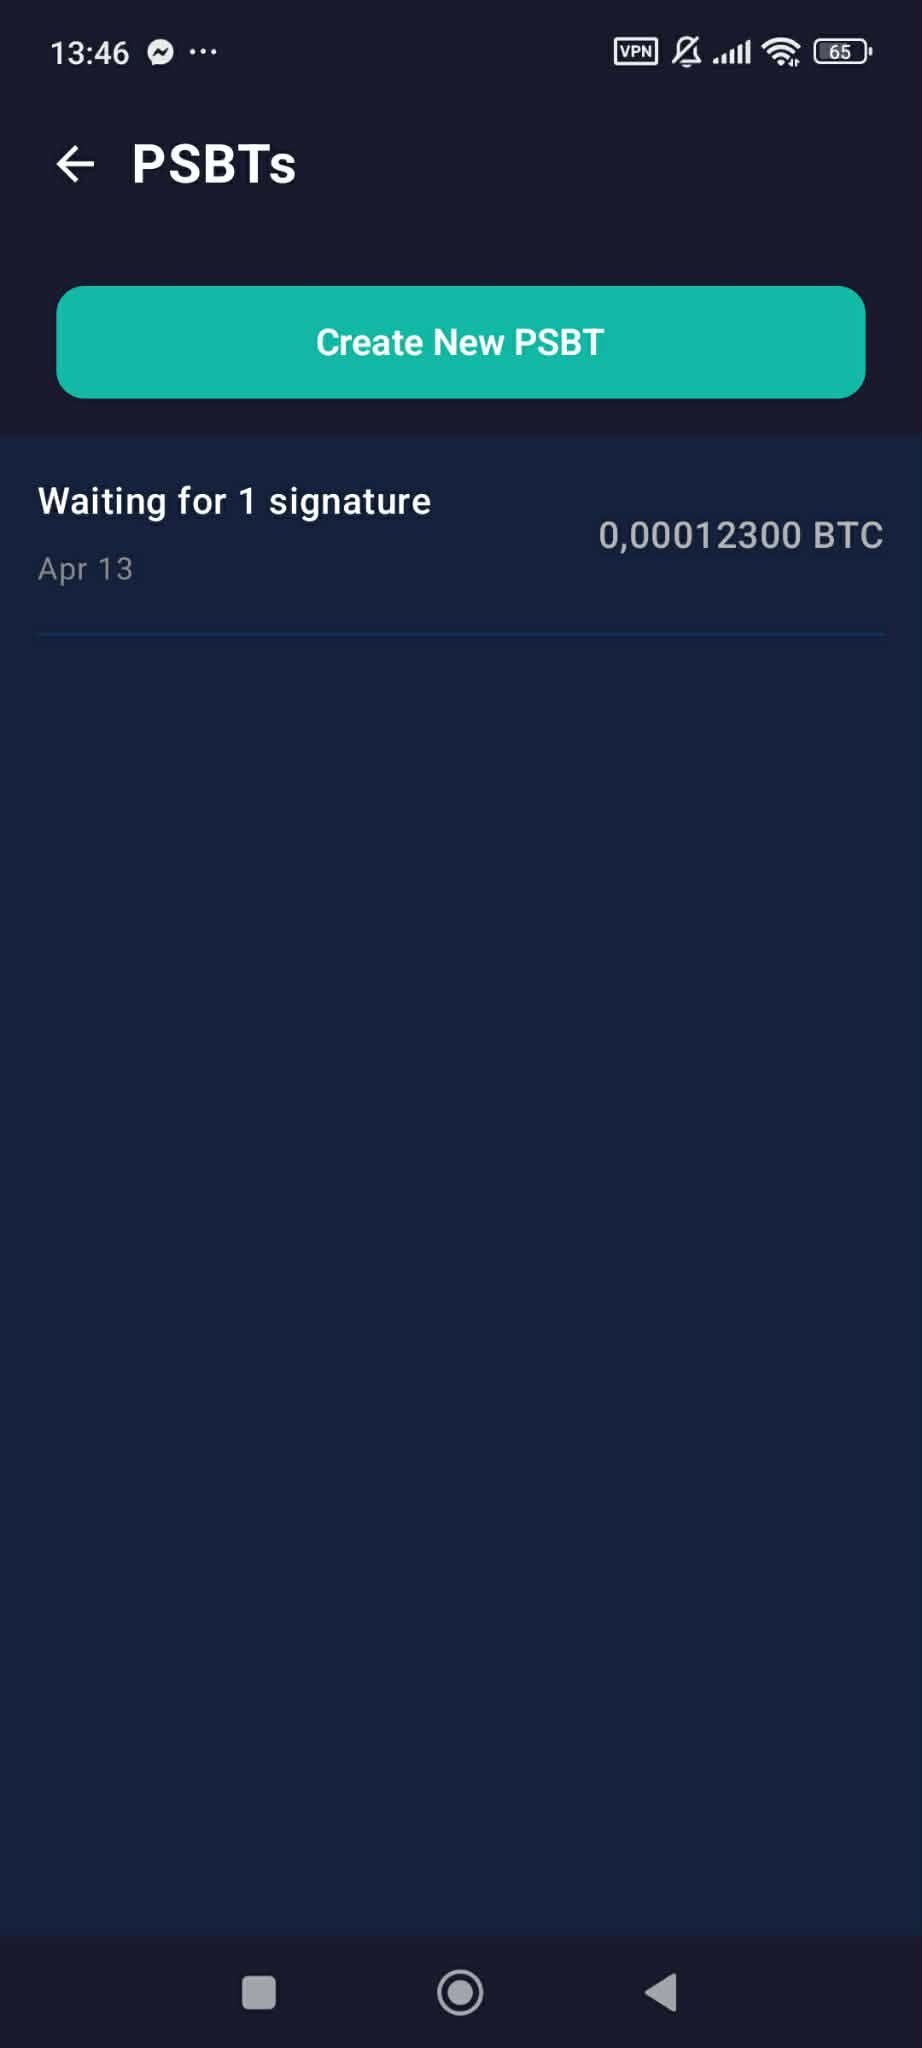
\includegraphics[height=0.22\textheight]{img/screen-psbt-list.jpeg}\hfill
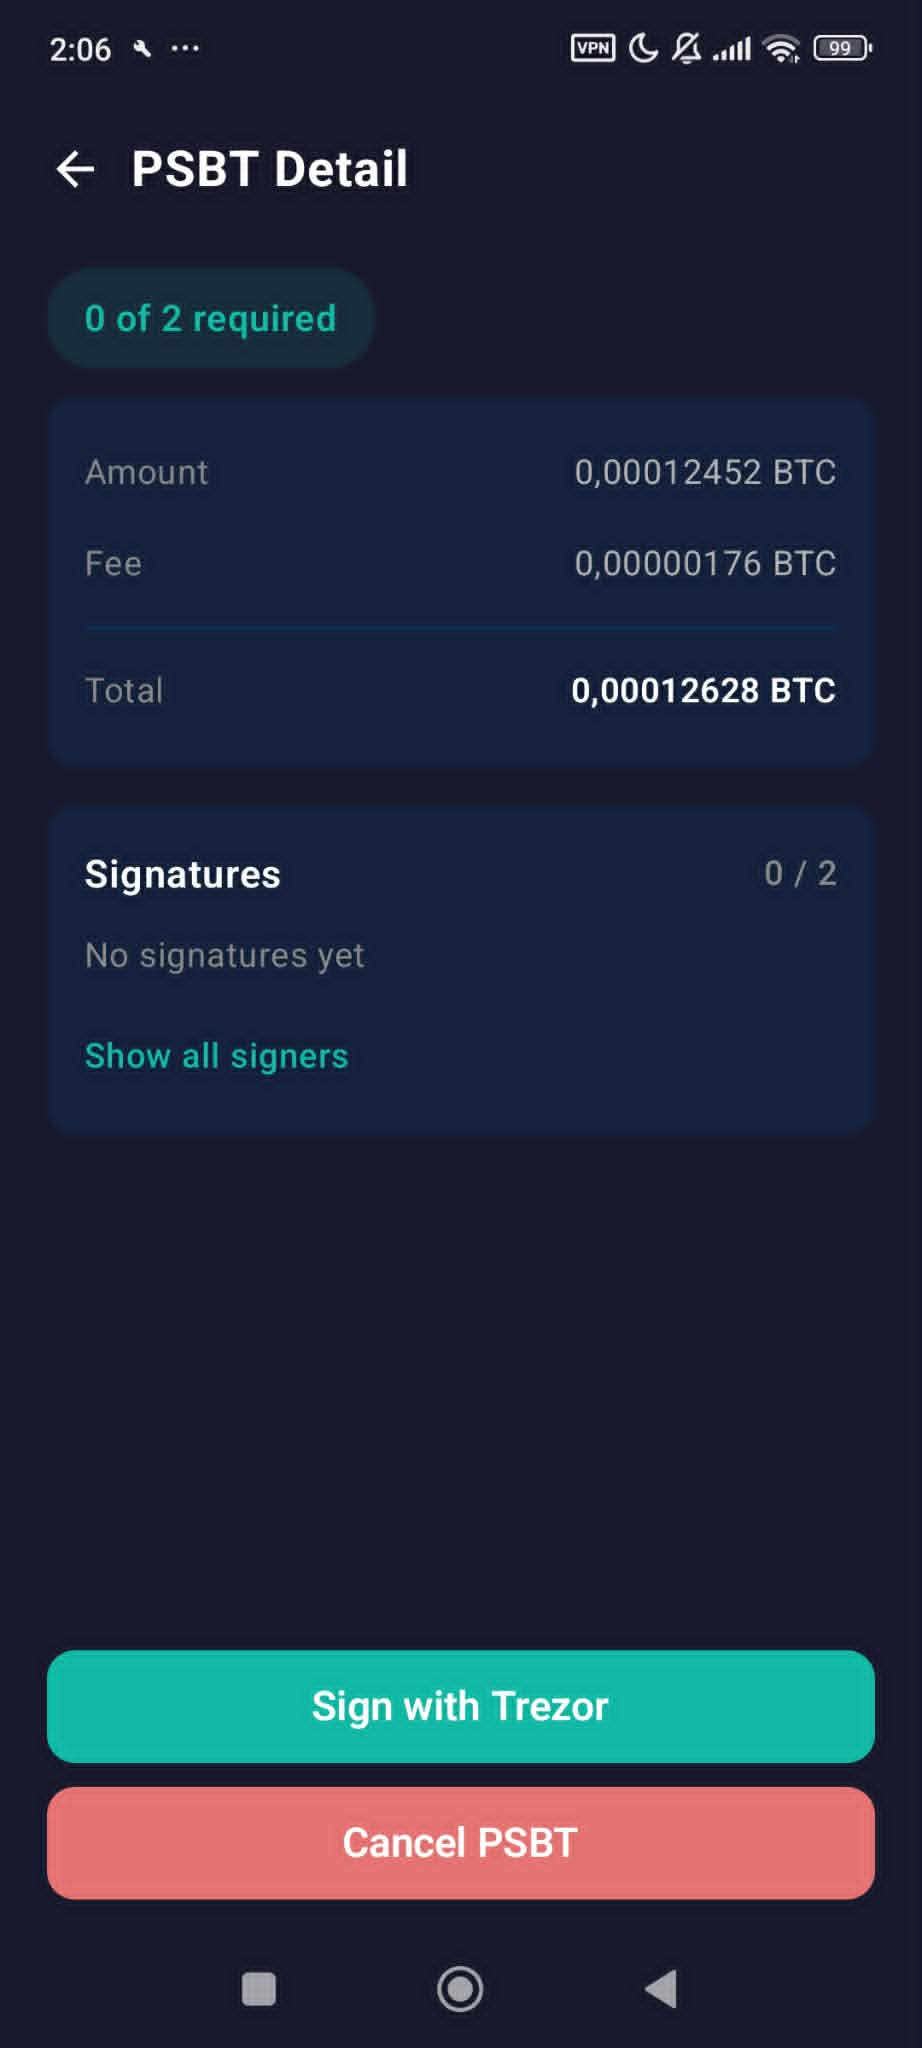
\includegraphics[height=0.22\textheight]{img/screen-psbt-detail.jpeg}\hfill
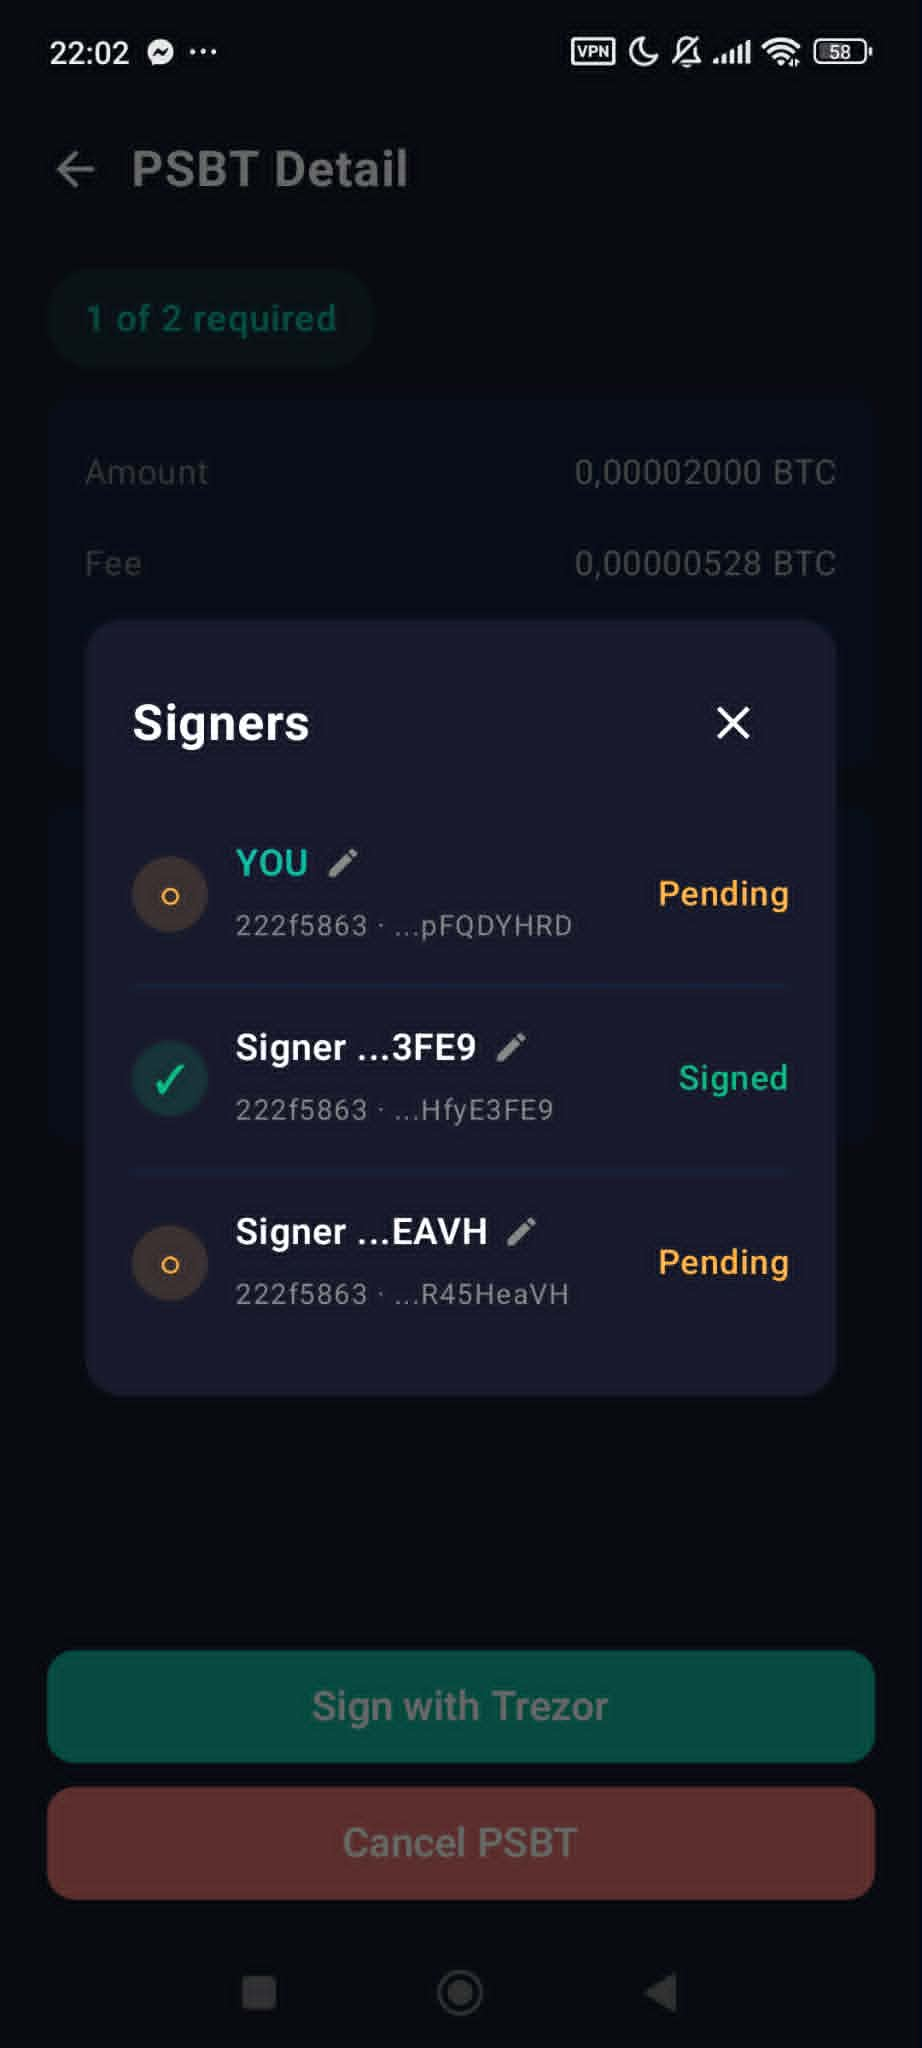
\includegraphics[height=0.22\textheight]{img/screen-psbt-signers.jpeg}\hfill
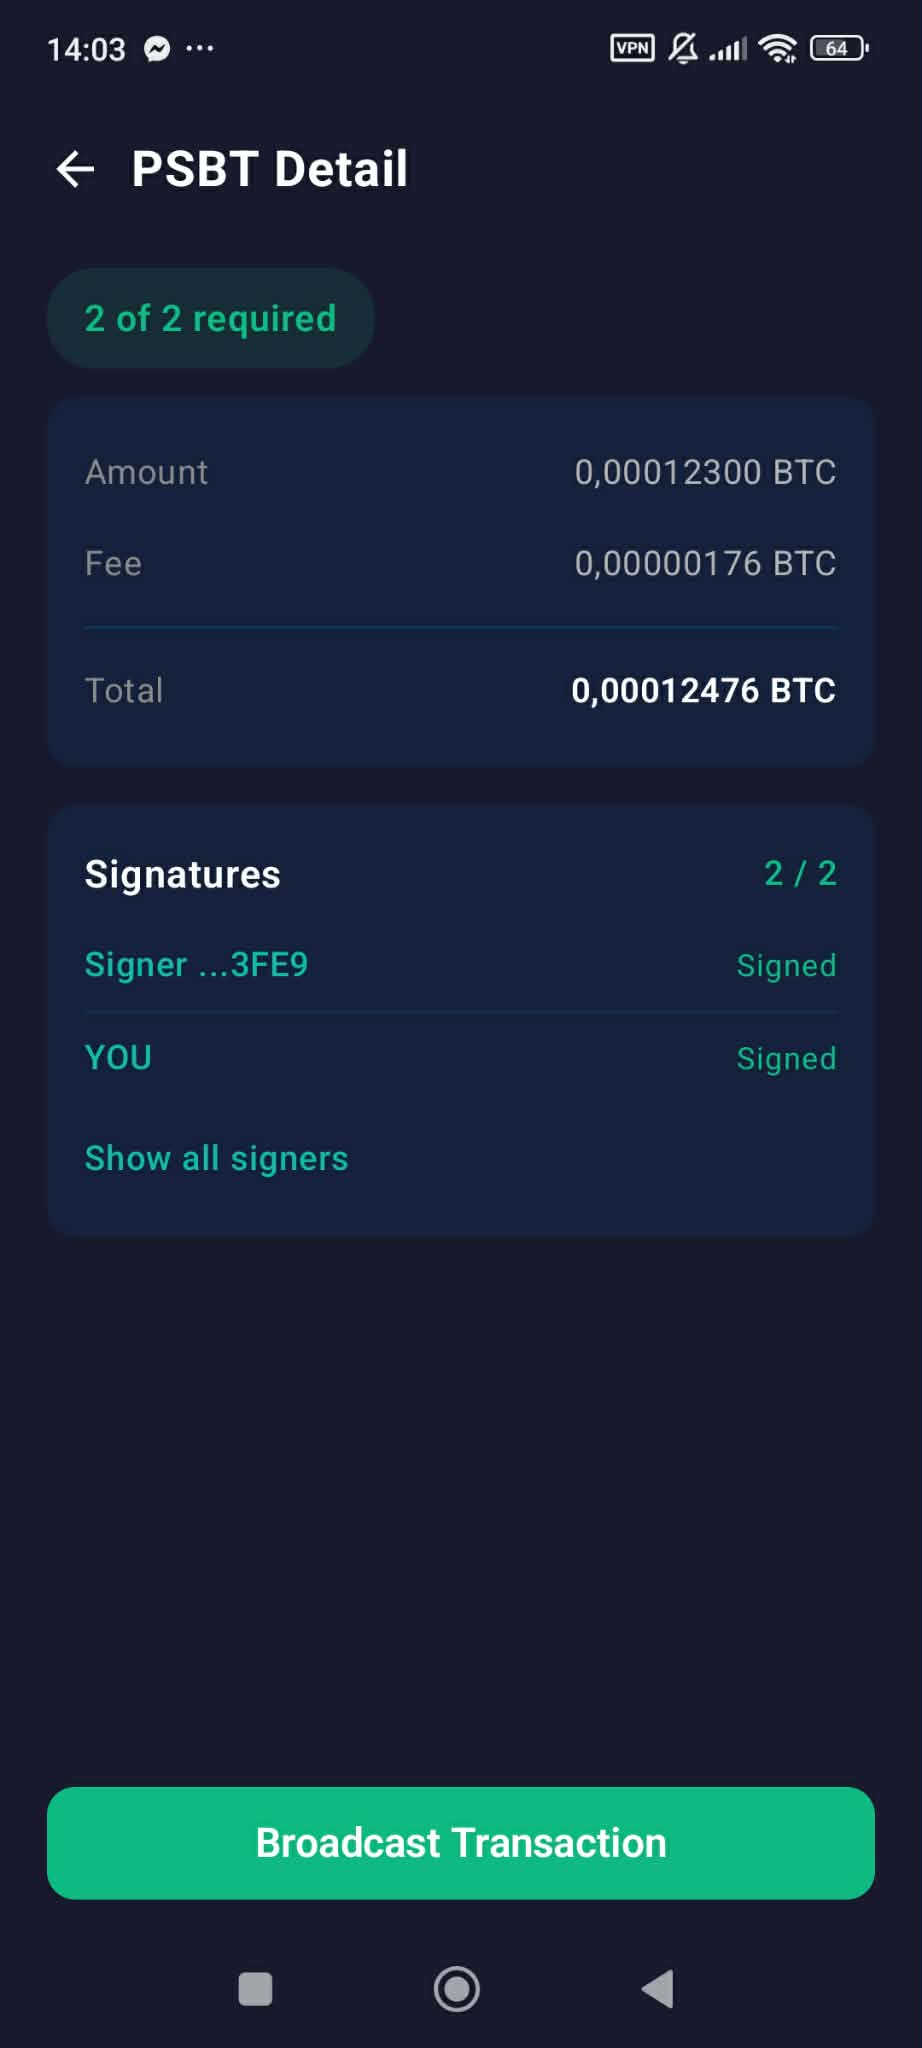
\includegraphics[height=0.22\textheight]{img/screen-psbt-broadcast.jpeg}
\caption[PSBT workflow]{PSBT workflow. Zleva: seznam PSBT transakcí;
detail PSBT bezprostředně po vytvoření (0 ze~2 podpisů) s~tlačítkem
\emph{Cancel PSBT} pro stažení návrhu před podpisem; dialog signerů
se stavy Signed~/~Pending a~příznakem \emph{YOU}; PSBT s~dosaženým
prahem (2 ze~2) připravené k~broadcastu.}
\label{fig:screen-psbt-flow}
\end{figure}

\textbf{Detail PSBT.}
Po kliknutí na konkrétní PSBT se otevře detailní obrazovka
(obrázek~\ref{fig:screen-psbt-flow}, uprostřed) se souhrnem částky,
poplatku a~celkové hodnoty transakce. Klíčovou součástí je přehled
podpisů -- barevný indikátor zobrazuje aktuální stav (například
\uv{1 of~2 required}) a~pod ním je seznam cosignerů s~informací, zda
každý z~nich již podepsal.

V~dialogu signerů (obrázek~\ref{fig:screen-psbt-flow}, vpravo, přístupném
přes odkaz \emph{Show all signers}) uživatel vidí u~každého cosignera jeho
stav, fingerprint a~zkratku veřejného klíče. Cosignerům je možné přiřadit
pojmenování (například \uv{Pepa}) stisknutím ikony tužky -- název se uloží
pouze pro aktuálně přihlášené zařízení a~ostatním cosignerům se nezobrazí,
aby osobní poznámky neprosakovaly mezi členy sdílené peněženky. Cosigner
odpovídající aktuálně přihlášenému účtu je označen příznakem \emph{YOU}.

Pokud transakce čeká na podpis aktuálního cosignera, zobrazí se tlačítko
\emph{Sign with Trezor}, které přesměruje uživatele do Trezor Suite Mobile.
Po stisknutí tlačítko zšedne a~popisek odráží aktuální fázi
(\emph{Waiting for Trezor\ldots} během čekání na callback,
\emph{Processing\ldots} při následném odesílání podpisů na backend),
což brání opakovanému spuštění deeplinku.
Návrh transakce, který ještě nebyl odeslán do sítě, lze tlačítkem
\emph{Cancel PSBT} stáhnout -- backend záznam smaže a~uvolní zarezervované
UTXO zpět k~použití v~jiné transakci. Po dobu čekání na Trezor se Cancel PSBT
skrývá a~místo něj se zobrazí nedestruktivní \emph{Cancel signing}, které
pouze ukončí čekání, aniž by draft smazalo -- případný pozdě dorazivší
podpis tak nepadne na neexistující záznam. Po broadcastu obě tlačítka mizí,
aby zůstal zachován audit záznam již odeslaných transakcí.

\textbf{Doplnění podpisu dalším cosignerem.}
Pro doplnění dalšího podpisu musí podepsat jiný cosigner. V~reálném nasazení
si druhý cosigner otevře tutéž transakci ve své vlastní instanci aplikace
napojené na společný backend; pro účely testování (kdy máme jeden Trezor
a~tři účty na něm) lze v~jedné instanci přepnout aktivní účet v~nastavení
pod položkou \emph{Switch Account}. Po přepnutí najde uživatel
rozpracovanou transakci v~seznamu PSBT u~odpovídající multisig peněženky,
otevře její detail a~stiskne \emph{Sign with Trezor} -- aplikace ho opět
přesměruje do Trezor Suite Mobile.

Po dosažení prahu~$M$ (obrázek~\ref{fig:screen-psbt-flow}, vpravo)
má PSBT kompletní sadu podpisů. Na~detailu PSBT zmizí tlačítko
\emph{Sign with Trezor} a~místo něj se objeví \emph{Broadcast
Transaction}. Po~jeho stisknutí aplikace zavolá na~backend endpoint
pro~broadcast, ten výslednou transakci propaguje přes
\texttt{blockchain-service} do~Bitcoinové sítě a~aplikace zobrazí
potvrzení s~identifikátorem transakce shodně jako u~singlesig
odeslání. Broadcast je tedy vždy explicitní akcí některého
cosignera na~detailu PSBT -- po~přijetí posledního podpisu se
transakce sama od~sebe neodesílá.

\textbf{Zrušení rozpracované transakce.} Pokud uživatel zjistí, že
transakce byla vytvořena s~chybnými parametry (například špatná
cílová adresa nebo částka), nebo cosigner z~jakéhokoli důvodu
nepodepíše, nabízí detail PSBT tlačítko \emph{Cancel PSBT}. Po
potvrzení v~dialogu aplikace zavolá \texttt{DELETE /psbt/\{id\}},
backend záznam smaže a~uvolní rezervaci utracených UTXO, takže je lze
znovu použít v~nové transakci. Tlačítko je dostupné jen u~PSBT, které
ještě nebyly broadcastnuty -- broadcastované transakce se uchovávají
jako auditní stopa. Bez této možnosti by opuštěná multisig konfigurace
držela své UTXO blokované až do automatického úklidu po~sedmi dnech
(viz sekci~\ref{sec:datovy-model}).


\chapter*{Závěr}
\addcontentsline{toc}{chapter}{Závěr}
\label{chap:zaver}

Cílem této práce bylo navrhnout a~implementovat mobilní aplikaci pro Android,
která umožní pokročilou správu Bitcoinových prostředků -- konkrétně podporu
multisignature transakcí ve schématu M-of-N, integraci s~hardwarovou peněženkou
Trezor a~manuální výběr UTXO -- a~zaplnit tak mezeru, kterou jsme v~analýze
existujících peněženek (viz~kapitolu~\ref{chap:related}) identifikovali na
mobilních platformách. Všechny tři stanovené cíle se podařilo naplnit;
ověření jejich funkčnosti popisujeme v~kapitole~\ref{chap:testovani}, kde jsme
mimo jiné provedli kompletní 2-of-3 multisig transakci od importu deskriptoru
přes postupné podepisování dvěma cosignery až po broadcast na Bitcoin testnet.

Výsledná aplikace se skládá z~šesti backendových mikroslužeb a~API Gateway
implementovaných v~jazyce Kotlin s~frameworkem Ktor~\cite{KtorFramework}
a~nativního Android frontendu postaveného na Jetpack Compose~\cite{JetpackCompose}.
Bezpečnostní model důsledně dodržuje princip, že server nikdy nedisponuje
privátními klíči ani jinými materiály, ze~kterých by je bylo možné odvodit --
veškeré podepisování probíhá výhradně na hardwarové peněžence, kterou
oslovujeme prostřednictvím deeplink protokolu Trezor Connect~\cite{TrezorConnect}
zprostředkovaného aplikací Trezor Suite Mobile~\cite{TrezorSuite}.
Pro distribuci částečně podepsaných transakcí mezi cosignery
využíváme standard PSBT~\cite{BIP174} a~konfiguraci multisig peněženky
přebíráme z~výstupních deskriptorů ve~formátu \texttt{wsh(sortedmulti(M,\ldots))}
podle BIP-380~\cite{BIP380} a~BIP-383~\cite{BIP383}. Tato volba zajišťuje
interoperabilitu s~existujícími desktopovými peněženkami -- typicky lze
vytvořit multisig konfiguraci ve Sparrow Wallet~\cite{SparrowWallet}, exportovat
deskriptor a~v~naší aplikaci jej importovat, čímž obě peněženky pracují nad
totožnou množinou adres.

Práce ukazuje, že kombinace pokročilých funkcí, kterou na desktopu poskytuje
Sparrow Wallet, je realizovatelná i~na mobilní platformě bez kompromisu
v~bezpečnostním modelu. Mobilní zařízení v~tomto uspořádání slouží jako
plnohodnotný koordinátor multisig transakcí (vytváří PSBT, sleduje stav
shromážděných podpisů, koordinuje broadcast), zatímco veškeré kryptografické
operace zůstávají izolovány na hardwarové peněžence cosignera. Nejvýraznějším
ústupkem oproti desktopovému řešení je delegace komunikace s~Trezorem na
externí aplikaci Trezor Suite Mobile, kterou jsme zvolili jako pragmatický
kompromis mezi rozsahem bakalářské práce a~kvalitou uživatelského prožitku;
důvody i~zvažované alternativy popisujeme v~sekci~\ref{sec:analyza-trezor}.

\section*{Hlavní přínosy práce}

Konkrétní přínosy práce shrnujeme do následujících bodů:

\begin{itemize}
\item \textbf{Mobilní peněženka kombinující multisig, coin control
  a~přímou integraci s~Trezorem bez privátních klíčů na~serveru.}
  Srovnání sedmi existujících řešení v~sekci~\ref{sec:comparison}
  ukázalo, že žádné z~analyzovaných mobilních řešení tuto kombinaci
  nenabízí; nejbližší konkurent BlueWallet~\cite{BlueWallet} podporuje
  multisig na~mobilu, ale komunikace s~hardwarovou peněženkou probíhá
  pouze přes manuální přenos PSBT souborů, bez přímé integrace přes
  deeplink protokol Trezor Connect~\cite{TrezorConnect}. Bezpečnostní
  model jsme ověřili kompletní 2-of-3 multisig transakcí na Bitcoin
  testnetu (viz~kapitolu~\ref{chap:testovani}).

\item \textbf{Engineering deeplink workflow s~Trezor Suite Mobile.}
  Asynchronní podepisování přes Android intenty vyžaduje řešení
  několika netriviálních problémů, jejichž postup není v~dokumentaci
  Trezor Connect~\cite{TrezorConnect} popsán: korelace odpovědí
  s~pending PSBT přes \texttt{requestId}, detekce odpovědi z~jiného
  Trezoru než toho přihlášeného (sentinel \texttt{WRONG\_DEVICE}
  s~auto-logoutem), rozlišení passphrase identity stejného fyzického
  zařízení podle fingerprintu xpub a~obnova stavu po~návratu uživatele
  z~aplikace třetí strany. Konkrétní implementace je popsána
  v~sekci~\ref{subsec:deeplink-workflow}.

\item \textbf{Identifikace implementačních úskalí PSBT a~Trezor
  workflow.} Při ladění jsme narazili na chyby, jejichž diagnostika
  vyžadovala detailní studium specifikací i~bezpečnostních patchů
  firmware Trezoru. Pole
  \texttt{PSBT\allowbreak \_\allowbreak IN\allowbreak \_\allowbreak NON\allowbreak \_\allowbreak WITNESS\allowbreak \_\allowbreak UTXO}
  je vyžadováno i~pro nativní SegWit vstupy počínaje firmware Trezor
  Model T 2.3.1 (resp. Trezor One 1.9.1) z~června 2020 jako mitigace
  BIP-143 SegWit fee útoku zveřejněného Saleemem Rashidem v~březnu
  2020~\cite{TrezorSegwitFix2020}; současný firmware modelů Safe 3, 5
  a~7 toto pravidlo přebírá. Standard BIP-174~\cite{BIP174} přitom
  toto pole pro SegWit vstupy označuje pouze za~volitelné
  (\enquote{\emph{can be present}}). U~deskriptoru
  \texttt{sortedmulti(\ldots)} je třeba podpisy ve~witness stacku
  řadit podle pořadí \emph{odvozených} klíčů, jak explicitně předepisuje
  BIP-383~\cite{BIP383} (\enquote{\emph{after all extended keys are
  derived}}); naivní seřazení xpubs jednou při parsování deskriptoru
  vede k~nevalidní transakci. Konečně předcházení reuse change adres
  vyžádalo vlastní mechanismus sledování stavu napříč rozpracovanými
  PSBT, který není pokryt ani Trezor Connect, ani PSBT formátem.
  Detaily nálezů a~jejich oprav jsou popsány v~sekci~\ref{sec:test-chyby}
  a~mohou posloužit dalším implementátorům.

\item \textbf{Interoperabilita s~peněženkami podporujícími výstupní
  deskriptory bez~importu klíčového materiálu.} Parser deskriptorů
  ve~formátu \texttt{wsh(sortedmulti(\ldots))} podle BIP-380~\cite{BIP380}
  a~BIP-383~\cite{BIP383} přijímá vstup od~jakékoli peněženky, která
  tento otevřený standard respektuje (například Sparrow Wallet, Bitcoin
  Core nebo Specter Desktop). Postup je univerzální: na~desktopu se
  vytvoří multisig konfigurace, exportuje deskriptor a~v~mobilní
  aplikaci se~importuje, čímž obě peněženky pracují nad~totožnou
  množinou adres bez~potřeby přenášet privátní klíče ani seedy mezi
  platformami. Funkčnost jsme ověřili proti Sparrow
  Walletu~\cite{SparrowWallet} jako referenční desktop implementaci
  (viz~sekci~\ref{sec:test-prostredi}).
\end{itemize}

\section*{Možnosti dalšího vývoje}

Aplikace je navržena s~ohledem na další rozšiřování a~několik konkrétních
směrů budoucího vývoje považujeme za přirozené pokračování této práce.

Nejvýznamnějším z~nich je \textbf{přímá komunikace s~hardwarovou peněženkou}
přes Android USB Host API. Současný stav, kdy aplikace deleguje podepisování
na Trezor Suite Mobile, je sice funkční, ale zhoršuje uživatelský komfort
nutností přepínat mezi dvěma aplikacemi a~zavádí závislost na~softwaru třetí
strany. Vlastní implementace by znamenala napsat USB transportní vrstvu
nad 64bajtovým paketovým protokolem Trezoru, kompletní sadu protobuf zpráv
podle aktuálního firmware a~stavový automat pro vícekolovou komunikaci typu
\texttt{SignTx -- TxRequest -- TxAck}, který Trezor používá kvůli omezené
paměti zařízení. Tento rozsah implementace odpovídá samostatnému projektu
přesahujícímu rámec bakalářské práce, proto jsme tento směr vědomě nepřevzali,
ale architektura aplikace
je na něj připravena -- veškerá komunikace s~Trezorem prochází přes interní
abstrakci \texttt{TrezorDeeplinkLauncher} popsanou v~sekci~\ref{sec:impl-detaily},
za~kterou se aktuální deeplink implementace dá nahradit přímou USB
komunikací bez zásahu do zbytku systému.

Druhým přirozeným rozšířením je \textbf{podpora dalších hardwarových peněženek},
zejména Ledger a~Coldcard. Architektura backendu je na~konkrétním modelu
Trezoru nezávislá -- pracuje s~PSBT a~výstupními deskriptory, což jsou
otevřené standardy podporované všemi zmíněnými výrobci. Podpora dalších
zařízení by tak vyžadovala práci pouze na straně mobilní aplikace,
především implementaci odpovídajících transportních vrstev.

Třetím směrem je \textbf{příprava na produkční provoz}. Aplikace již
podporuje přepínání mezi testnetem a~mainnetem přímo z~přihlašovací
obrazovky a~backend automaticky komunikuje s~odpovídajícím blockchainovým
API (Mempool.space pro testnet, Blockstream
Esplora~\cite{BlockstreamEsplora} pro mainnet). Před reálným nasazením
s~finančními prostředky by však bylo vhodné provést bezpečnostní audit
a~rozšířit \textbf{automatizovanou testovací sadu}. Jednotkové testy nad
deterministickými částmi (PSBT a~Trezor Connect parametry, audit trail
podpisů, derivace adres, parser deskriptorů, vystavování a~rotace JWT
tokenů, klasifikace transakcí a~retry logika blockchain klienta) jsme
do~práce zahrnuli a~popsali v~sekci~\ref{sec:test-unit}; chybí
end-to-end pokrytí pomocí Trezor emulátoru, které jsme z~důvodů
diskutovaných v~sekci~\ref{sec:test-pristup} odložili na další vývoj.

Mezi další užitečná rozšíření patří podpora náhradních strategií výběru
UTXO (například algoritmus Branch and Bound), možnost připojit aplikaci
k~vlastnímu Bitcoin uzlu místo veřejných API, podpora schématu Taproot
(BIP-86) a~rozšíření o~zobrazení podrobných statistik a~grafů pohybů
prostředků.


%%% Příloha A: Obsah elektronické přílohy

\appendix
\chapter{Obsah elektronické přílohy}
\label{app:struktura}

Elektronická příloha obsahuje kompletní zdrojové kódy aplikace potřebné
pro její sestavení a~spuštění. Struktura kořenového adresáře je následující:

\bigskip
\begin{description}
\item[\texttt{wallet-backend/}] Backendové mikroslužby implementované
  v~jazyce Kotlin s~frameworkem Ktor. Adresář obsahuje:

  \begin{description}
  \item[\texttt{api-gateway/}] API Gateway -- vstupní bod pro mobilní
    aplikaci, JWT autentizace, směrování požadavků na mikroslužby.
  \item[\texttt{auth-service/}] Autentizační služba -- vydávání JWT
    tokenů, správa identit zařízení.
  \item[\texttt{wallet-registry/}] Správa peněženek -- import deskriptorů,
    derivace adres, správa cosignerů.
  \item[\texttt{explorer-service/}] Agregace dat -- zůstatky, historie
    transakcí, UTXO pro konkrétní peněženku.
  \item[\texttt{psbt-service/}] PSBT workflow -- tvorba, podepisování
    a~broadcast transakcí.
  \item[\texttt{blockchain-service/}] \hfill \\
    Proxy k~blockchainovým API (Mempool.space, Blockstream Esplora).
  \item[\texttt{price-service/}] Směnný kurz BTC vůči fiat měnám
    (CoinGecko API).
  \item[\texttt{docker-compose.yml}] Definice všech kontejnerů pro
    spuštění celého backendu jedním příkazem
    \texttt{docker compose up --build -d}.
  \item[\texttt{init-db.sql}] Inicializační skript vytvářející databáze
    při prvním spuštění.
  \end{description}

\item[\texttt{wallet-frontend/}] Mobilní aplikace pro Android
  implementovaná v~jazyce Kotlin s~frameworkem Jetpack Compose. Klíčové
  balíčky:

  \begin{description}
  \item[\texttt{core/api/}] HTTP klient a~repozitáře pro komunikaci
    s~backendem.
  \item[\texttt{core/trezor/}] Integrace s~hardwarovou peněženkou Trezor
    prostřednictvím deeplink protokolu Trezor Connect.
  \item[\texttt{core/session/}] Správa stavu přihlášení a~aktivní
    peněženky.
  \item[\texttt{feature/trezorconnect/}] Přihlašovací obrazovky --
    připojení Trezoru a~výběr účtu.
  \item[\texttt{feature/wallet/}] Hlavní funkcionalita -- dashboard,
    odeslání a~příjem prostředků, coin control, multisig peněženky,
    PSBT workflow.
  \end{description}

\item[\texttt{README.md}] Stručný popis projektu a~návod na sestavení.
\end{description}

\bigskip
\noindent\textbf{Požadavky pro sestavení.}
Pro spuštění backendu je potřeba Docker Engine a~Docker
Compose~\cite{Docker}. Pro sestavení mobilní aplikace je potřeba Android
Studio s~Gradle a~Android SDK (minimální API~24). Podrobný postup
spuštění popisuje kapitola~\ref{chap:uzivatelska}.


%%% Seznam použité literatury
\include{literatura}

%%% Obrázky v práci
%%% (pokud jich je malé množství, obvykle není třeba seznam uvádět)
\listoffigures

%%% Tabulky v práci (opět nemusí být nutné uvádět)
%%% U matematických prací může být lepší přemístit seznam tabulek na začátek práce.
\listoftables

%%% Použité zkratky v práci (opět nemusí být nutné uvádět)
%%% U matematických prací může být lepší přemístit seznam zkratek na začátek práce.
\chapwithtoc{Seznam použitých zkratek}

\begin{description}
\item[API] Application Programming Interface -- rozhraní pro komunikaci mezi aplikacemi
\item[BIP] Bitcoin Improvement Proposal -- návrh na vylepšení protokolu Bitcoin
\item[BTC] Bitcoin -- kryptoměna
\item[DER] Distinguished Encoding Rules -- binární formát kódování kryptografických dat
\item[HD] Hierarchical Deterministic -- hierarchická deterministická derivace klíčů
\item[HMAC] Hash-based Message Authentication Code
\item[HTTP] Hypertext Transfer Protocol
\item[JSON] JavaScript Object Notation -- formát pro výměnu dat
\item[JWT] JSON Web Token -- standard pro autentizační tokeny
\item[MVVM] Model-View-ViewModel -- architektonický vzor
\item[P2WPKH] Pay-to-Witness-Public-Key-Hash -- typ SegWit výstupu pro singlesig
\item[P2WSH] Pay-to-Witness-Script-Hash -- typ SegWit výstupu pro multisig
\item[PSBT] Partially Signed Bitcoin Transaction -- formát pro částečně podepsané transakce
\item[REST] Representational State Transfer -- architektonický styl webových API
\item[SegWit] Segregated Witness -- protokolové vylepšení Bitcoinu
\item[SHA-256] Secure Hash Algorithm -- kryptografická hashovací funkce
\item[UI] User Interface -- uživatelské rozhraní
\item[URI] Uniform Resource Identifier
\item[UUID] Universally Unique Identifier -- univerzálně unikátní identifikátor
\item[UTXO] Unspent Transaction Output -- nepoužitý transakční výstup
\item[vB] Virtual Byte -- jednotka velikosti transakce po SegWitu
\end{description}

\end{document}
